\clearpage
\section{Event Selection} 

\subsection{Trigger Selection} \label{sec::Samples::trigger}
The missing ET trigger (MET trigger) is primarily used throughout the analysis.
Since the lowest unprescaled trigger kept evoloved according to the increased instantaneous luminosity during the 2016 data taking, a number of different triggers are used in combination.
The list of the triggers are shown in Tab. \ref{tab::SRdefinition::METtriggers},

\tabsmall{ccc|cc}{

\hline
Period      &  Peak lumi. [cm$^{-2}$ s$^{-1}$]  &  Int. lumi. [fb$^{-1}$]  &   L1 (HLT) item       &  L1/HLT/Off-line threshold [GeV]  \\
\hline
2015        &  0.50 $\times 10^{34}$                                     &  3.19                         &   L1XE50 (xe70\_mht)   &  50 / 70 / 200  \\
2016 A-D1   &  0.99 $\times 10^{34}$                                     &  6.12                         &   L1XE50 (xe90\_mht)   &  50 / 90 / 200   \\
2016 D1-F1  &  1.03 $\times 10^{34}$                                      &  6.55                         &   L1XE50 (xe100\_mht)  &  50 / 100 / 200  \\
2016 F2-    &  1.21 $\times 10^{34}$                                      &  20.2                         &   L1XE50 (xe110\_mht)  &  50 / 110 /  200   \\
\hline
}
{Summary of MET triggers used in the analysis along the peak luminosity evolution. Corresponding on-line and off-line threshold are shown altogether.}
{tab::SRdefinition::METtriggers}

% needed description 
% off-line MET -> cluster based
% on/off-line definition
%Taking the advantage that most of the targeted signal models result in large missing ET (MET) due to the presecnce of LSPs, the lowest unprescaled MET trigger (HLT\_xe110\_mth\_XE50) is used for triggering events throughout the analysis. 

The efficiency curve as function of off-line $\met$ is shown in Fig. \ref{sec::SRdefinition::METtrig} with the example of HLT\_xe100\_mht.
Thanks to the fact that MET is calculated from global information of an event, rather than the feature of a single particular particle, the plateau efficiency amounts almost 100 $\%$. 
This is a significant advantage over the use of leptonic trigger where efficiency is typically $70\% \sim 90\%$. 
Generally the downside of MET trigger is on the other hand its slow turn-on in terms of the off-line MET that needs nearly $200 \gev$ to assure the plateau efficiency despite much lower trigger threshold ($<110$ GeV). This is due to the deteriorated resolution of on-line MET which is purely based on calorimeter clusters, with respect to the off-line one which is take into muons and soft tracks into account. The signal acceptance by the trigger requirement is  $>95\%$ except when gluino mass and LSP mass are compressed. Nevertheless, given that it is impossible for such signal to be discriminated against background without the MET generated by associated ISRs, the loss in trigger is not problematic. \\

%The turn-on also has dependency on event topology and kinematics due to varying MET resolution in particular sensitive to magnitude of jet activity, however this does not affect the plateau efficiency. Fig. \ref{fig::SRdefinition::metTrigEff} shows turn-ons with different jet multiplicity. \\

The single-lepton trigger (SLT) is also used for supplemental purpose, including the efficiency measurement of MET trigger and closure tests of data-driven background estimation. The trigger turn-on is about $28\gev$ ($26\gev$) for single-electron (muon) in its transverse momentum and $30\gev$ ($28\gev$) is required as off-line threshold. \\


\fig[160]{SRdefinition/trigEff/metTrig_huajie.pdf}
{Turn-on of MET trigger HLT\_xe100\_mht simulated or measured using $\wjets$ events by performing the tag-and-probe technique. (a) events with exactly one muon, and (b) events with exactly one electron.}
{sec::SRdefinition::METtrig}


% -------------- MET trigger eff.  
%\begin{figure}
%  \begin{center}
%    \includegraphics[width=100mm]{figures/SRdefinition/trigEff/metTrigEff_lepTrigTag.eps}
%    \captionof{figure}{Efficiency curve of MET trigger measured with data by tagging a lepton with $p_{T}(\ell_{1})>35\gev$ firing the single-lepton trigger.}
%    \label{fig::SRdefinition::metTrigEff}
%  \end{center}
%\end{figure}






\subsection{Event Cleaning and the Pre-selection} \label{sec::SRdefinition::eventCleaning}
Event cleaning is applied to get rid of funky data events that are either in bad quality due to inappropriate detector status and badly measured objects, or with objects stemming from somewhere other than the hard collision such as cosmic muons and beam-induced background. 
As those events could result in extraordinary observables, for instance extremely high jet pt or MET, they are generally critical for search analyses probing the high-end of kinematics where only a few background events in signal regions are in discussion where therefore even a single event of the accidental contamination makes huge impact on the final result. The list of procedure and cut efficiencies are summarized in Tab. \ref{tab::SRdefinition::EvtCleaning}. 

\tab{ c | c | c }{
  \hline
                       Cut              &  Efficiency (Data) $[\%]$   &  Efficiency (MC, $\ttbar$) $[\%]$  \\
  \hline
  \hline
  Veto bad lumi-clocks                  & 95.12                            &  100.0        \\
  Veto bad DAQ events                   & 99.81                            &  100.0        \\
  Veto events with no primary vertex    & 100.0                            &  100.0        \\
  Veto events with cosmic muons         & 95.83                            &  98.52        \\
  Veto events with badly measured jets  & 99.49                            &  99.65        \\
  Veto events with badly measured muons & 99.99                            &  98.56        \\              
  \hline
}
{List of cuts applied as event cleaning. Data and MC shows different efficiencies up-to the top four since MC does not emulates bad data quality and cosmic muons in it.}
{tab::SRdefinition::EvtCleaning}

Lumi-blocks with more than $10\%$ of the detector in the bad status are firstly removed. 
Events affected by noise bursts in LAr and SCT,  corrupted data transmission in LAr and the Tile calorimeter are then vetoed subsequently. 

%Event cleaning for badly measured objects applied rather conservatively giving that they could easily generate large fake MET that makes itself highly signal-like.
Cosmic muon are vetoed by requiring the muon track passing reasonably close-by the primary vertex i.e.
$$
|z_0| < 1\, \mathrm{mm}, \,\,\, d_0<0.2\, \mathrm{mm}.
$$
The beam induced backgrounds are events with muons that are generated by the secondary cascades of protons traveling upstream of the interaction point. The energy depositions created by these muons can be reconstructed as jets with energy as high as the beam energy therefore becomes highly signal-like. To reject the fake jets, event with jets flagged as ``BadLoose'' described in \cite{BadJetCriteriaATLAS2015} are vetoed. \\

Badly measured high energy muons are also the source of fake high MET ranging upto a few TeV.
Bad muons are defined as muons with $\sigma(q/p) / (q/p) > 0.2$ where $q/p$ is the track fitting parameter and $\sigma(q/p)$ is the error.a
The entire events will be vetoed if containing at least one bad muon.


Fig. \ref{fig::SRdefinition::badMuonVeto} demonstrate the performance of bad muon veto. While bad muon events typically peak in $\Delta \phi (l,\met)$ since the fake MET aligns with the muon, it is exclusively resolved by the veto. Also, the role of bad muon veto is shown to be very important in this analysis as the 1-muon high MET phase space generally suffers from severe contaminaton by bad muon events upto about 20$\%$ (90$\%$) with  $\met>1(2)\tev$.  \\

\begin{figure}[h]
  \centering
%    \subfigure[]{\includegraphics[width=0.48\textwidth]{figures/SRdefinition/badMuons/lep1Pt_met1TeV.pdf}}
    \subfigure[]{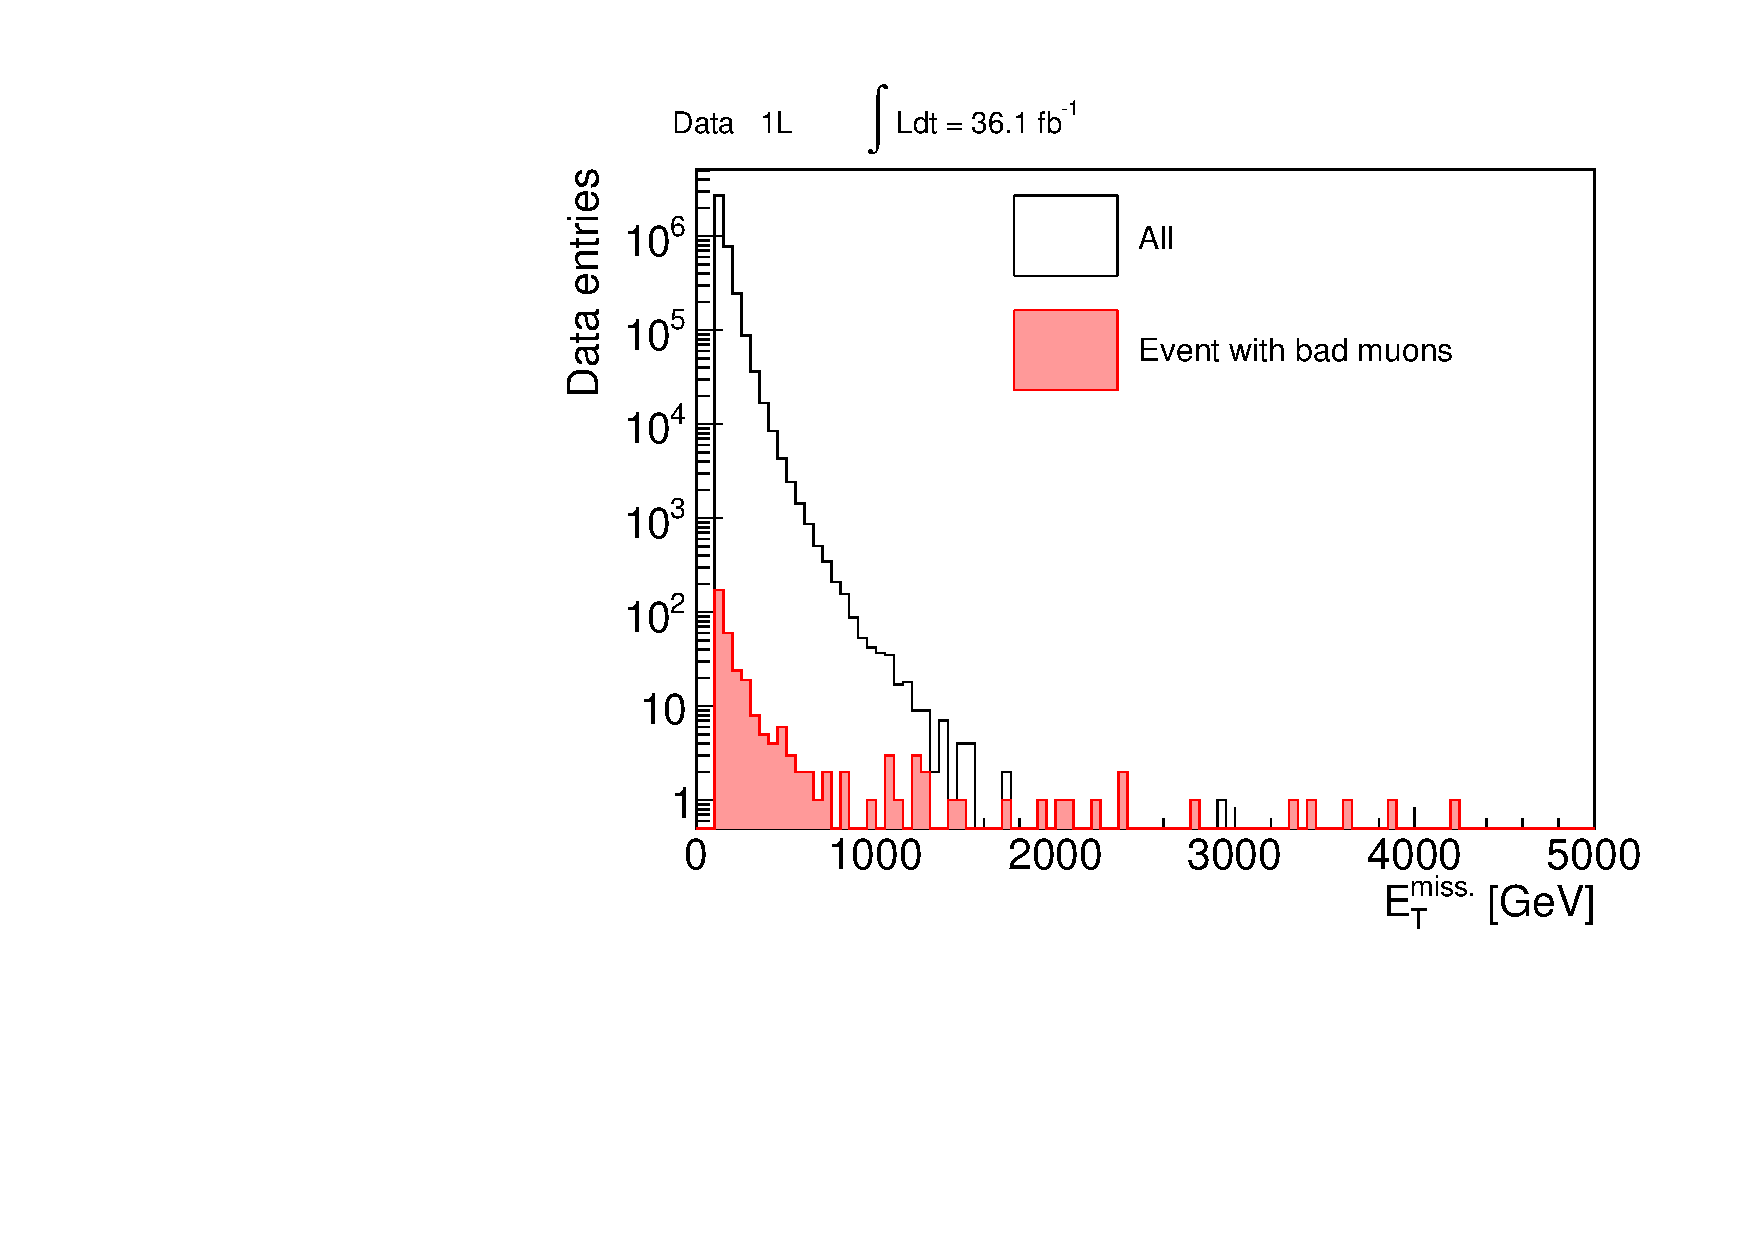
\includegraphics[width=0.48\textwidth]{figures/SRdefinition/badMuons/met_met0TeV.pdf}}
    \subfigure[]{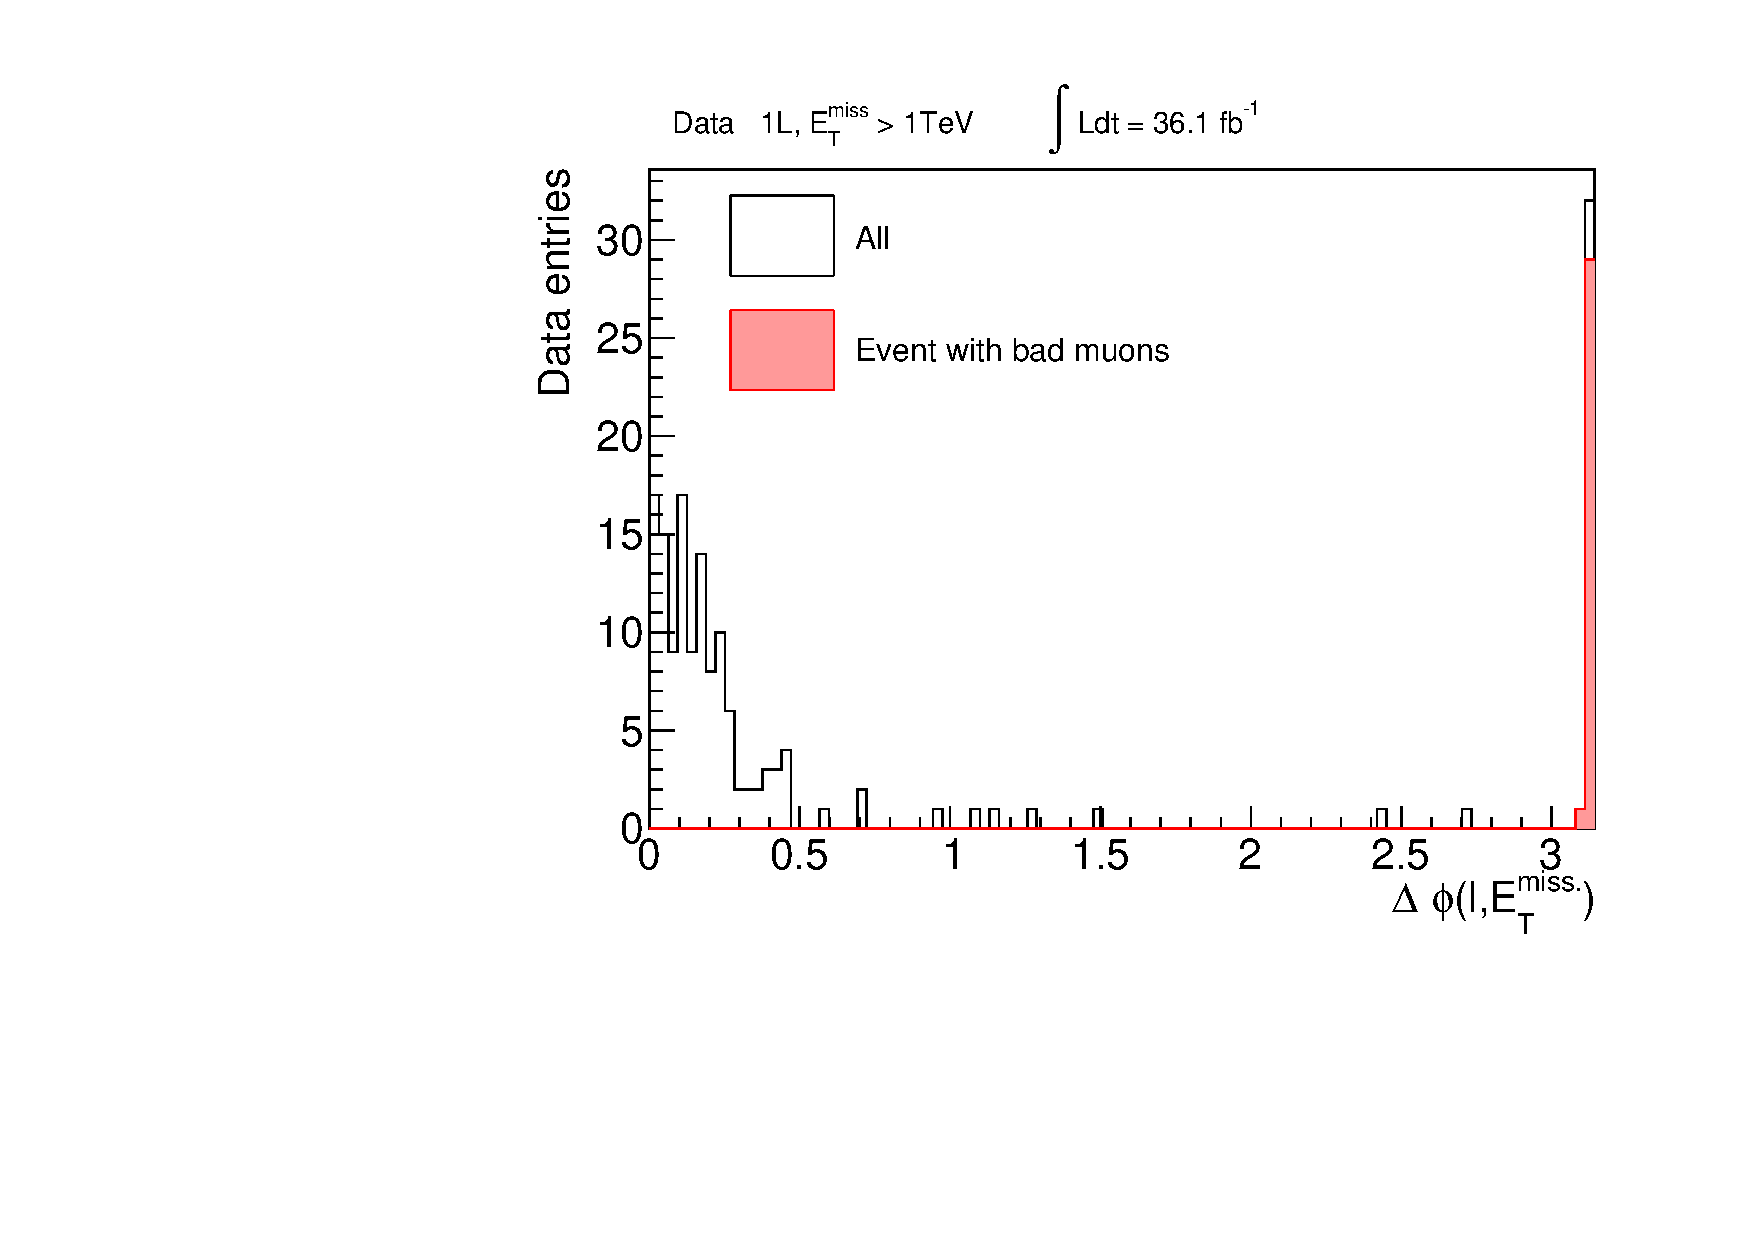
\includegraphics[width=0.48\textwidth]{figures/SRdefinition/badMuons/dPhi_met_lep_met1TeV.pdf}}
    \caption{(a) MET distribution after requiring exactly one signal muon and MET trigger, and (b) $\Delta \phi (l,\met)$ distribution with $\met>1\tev$ being applied. The pink histogram corresponds to events dropped by the bad muon veto. The veto looks working reasonably considering the apparent spike due to the fake MET: $\Delta \phi \sim \pi$ is cleared.}
    \label{fig::SRdefinition::badMuonVeto}
\end{figure}

The pre-selection is the common selection for all the signal regions in the analysis, which is defined as Tab. \ref{tab::SRdefinition::Preselection}.
\tab{ c }{
  \hline
  Event cleaning \\
  Pass the MET trigger and $\met>250\gev$ \\
  At least one signal electron (muon) with $\pt>7(6)\gev$. \\
  At least two jets with $\pt>30\gev$. \\
  \hline
}
{List of requirements for the 1-lepton pre-selection.}
{tab::SRdefinition::Preselection}

%%%%%%%%%%%%%%%%%%%%%%%%%%%%%%%%%%%%%%%%%%%%%
\subsection{Signal Region Definition}
\subsubsection{Binning Strategy}
To inclusively address to all the 45 decay models and all possible mass spectra, a set of tailored multi-bin signal regions (SRs) are employed.
Specifically, different decay models are covered by splitted the signal regions in terms of b-jet multiplicity (``categories''), 
and various scenario of mass spectra in the models are coped with the division in terms of kinematical cuts (``towers''). 
SR bins are basically designed to be exclusive for each other, aiming at an easy combination afterward so that no signals are lost due to the binning. \\

The definition of the b-jet based categories: b-vetoed (BV), b-tagged (BT) and 3B follows Tab. \ref{tab::SRdefinition::categoriesDef}. The main customers of these categories are respectively the models in Tab. \ref{tab::Introduction::modelsBV}, \ref{tab::Introduction::modelsBT} and \ref{tab::Introduction::models3B} in Sec. \ref{sec::Introduction::targetModels}, which are referred as ``BV'', ``BT'' and ``3B'' benchmark models from now on. 
The b-jet multiplicity for the reference signal models versus background at the pre-selection level is shown in Fig. \ref{fig::SRdefinition::nB}.
Note that despite a fraction of signal events falling into other categories than the benchmarked one, they will not be wasted thanks to the combined fit performed in deriving the final result.
As the S/N ratio and the background kinematics in BV/BT are found to be more or less similar, further kinematical selections in those categories are set to identical for simplicity. 
On the other hand, different selectiton strategy is adopted for the 3B categories since the background level is significantly lower and also the composition is very different. \\

%%%
\tab{ c | c | c }{
\hline
Category    & b-jet multiplicity   & Main background \\ 
\hline
\hline
B-vetoed (BV) & 0        & $\wjets$ \\
B-tagged (BT) & 1-2      & $\ttbar$ \\
3B            & $\geq 3$ & $\ttbar$, $\ttbar+cc/bb$ \\
\hline
}
{The definition of the b-jet based categories and the main backgrounds there.}
{tab::SRdefinition::categoriesDef}
%%%
\fig[110]{SRdefinition/discVar/nBJet30__Precut.pdf}
{B-tagged jet multiplicity for the standard model backgrounds and the reference signals (QQC1QQC1 for the BV, QQC1BTC1 for the BT and TTN1TTN1 for the 3B categories respectively) after the 1-lepton pre-selection.}
{fig::SRdefinition::nB}
%%%

\clearpage
The BV/BT categories are further divided into 4 ``towers'', to tackle the 4 typical configurations of the mass spectra for gluino and the LSP (and the intermediate EW gauginos in case of 1-step decays). The relation is schematized in Fig. \ref{fig::SRdefinition::binning_BTBV}, with the benchmark model ``QQC1QQC1'' being the example.
Each of them is further detailed as below:

\begin{enumerate}
\item The mass of intermediate EW gaugino is roughly in the middle of those of gluino and the LSP ($x \sim 1/2$).
This is the most standard configuration where particles from both gluino and the intermediate EW gaugino decays are hard enough to pass the criteria of hard lepton ($>35\gev$) and jets ($\pt>30\gev$). As the signals targeted by the BV/BT categories typically result in $4-10$ jets at the tree-level, a tower \textbf{6J} with $\nJetNoGev \geq 6$ is defined. 

\item Gluino and EW gauginos are all compressed. 
From either trigger and background separation point of view, hard ISRs are indispensive for probing this type of signatures so that the $\tilde{g}\tilde{g}$ system gets kicked and resulting in large MET. On the other hand, as the kicked gluinos are typically enough heavy to be non-relativistic, the transverse momentum of the boosted $\tilde{g}\tilde{g}$ system is almost solely converted into MET. As a result the particles from gluino decays stay soft. The \textbf{2J} tower consisting of a soft lepton, at least two hard jets and large MET is defined for targeting the signature.

\item,4 The intermediate EW gaugino and either gluino or LSP are compressed ($x \sim 0, 1$). 
There are also extreme cases where the intermediate EW gaugino mass is degenerate toward either of gluino or LSP and decoupled from the other. Two signal region towers: \textbf{$High-x$} and \textbf{$Low-x$} are employed to cover the scenarios. 
\end{enumerate}

Similar discussion holds for direct gluino decay models as well i.e. the tower \textbf{2J} covers the scenario of compressed mass spectra while the tower \textbf{6J} is used for general cases. \\

In contrast to the BV/BT category, the 3B does not undergo the additional classification in towers since the targeted signal models usually involve top quarks that can result in hard jets, leptons and MET. 
Therefore the kinematics does not dramatically vary between the mass configurations unless the top-quarks are on-shell.
The only exception is when gluino and the intermediate EW gaugino get compressed, and the top-quarks turn to off-shell ending up in soft decay particles.
However such events are then covered by the BT towers instead, thanks to the dropped $\geq 3$ b-jet acceptance according to the decreasing b-quarks' $\pt$. \\ 

To summarize, 5 towers (2J/6J/Low-x/High-x/3B) are defined in total out of 3 categories (BV/BT/3B) as in Tab. \ref{tab::SRdefinition::towersDef}. 
%The sensitivity converage by each signal region tower on the mass grid of the signal models are shown in Fig. \ref{fig::SRdefinition::towerCoverage}.

%%%%%%%%%%
\fig[160]{SRdefinition/EventSelection/binning_BTBV.eps}{The 4 signal region towers for the BT/BV categories, and their targeted mass configuration.}{fig::SRdefinition::binning_BTBV}

%%%
%\tab{ c | c | c | c | c }{
\tab{ c | c | c | c }{
\hline
%Category & Tower    & Electron (muon) $\pt$ [GeV]  &  $\nJet$ & Jet $\pt$ [GeV]\\ 
Category & Tower    & Electron (muon) $\pt$ [GeV]  &  $\nJet$  \\ 
\hline
\hline
      & 2J     & $\in [7(6), 35] $  & $\geq 2$ \\ \cline{2-4}
BV/BT & 6J     & $>35$              & $\geq 6$ \\ \cline{2-4}
      & Low-x  & $\in [7(6), 35] $  & $\geq 4$ \\ \cline{2-4}
      & High-x & $>35$              & $\geq 4$ \\
\hline
3B    & 3B     & $>15$              & $\geq 7$ \\
\hline
}
{List of defined towers in each b-category and t kinematical selection required. \textbf{2J} and \textbf{6J}, \textbf{Low-x} and \textbf{High-x} are orthogonal to each other. \textbf{3B} are orthogonal to all the other towers.}
{tab::SRdefinition::towersDef}
%%%


\clearpage
Finally, the towers further experience the binning in terms of $\meffInc := \met + \sum_{i} p_T (j_i)$ to accommodate different absolute scale of mass splitting. 
The ``2J/6J'' and ``3B'' tower are segmeted into 3 and 2 bins respectively while ``Low-x'' and ``High-x'' are single-binned as their low $\meffInc$ bins have too much overlap with ``2J'' and ``6J'' in phase space which does not provide unique sensitivity. The bin widths of $\meffInc$ are set to be $400\gev-500\gev$ driven by the width of $\meffInc$ distribution for signals that the lower $\meffInc$ bins typically target ($\dmg = 1\tev \sim 1.5\tev$). The ``3B'' tower enjoys an exceptionally wider bin width with $750\gev$, compromissing with limited of statistics in corresponding control regions. \\
%The lower bound of the last $\meffInc$ 

To conclude, the signal regions end up in 5 tower-structured bins as schematized as Fig. \ref{fig::SRdefinition::SRbinning}, where $3 \times 2$ bins in $\meffInc \times \mathrm{(BV/BT)}$ reside in the tower \textbf{"2J''} and \textbf{"6J''}, $1 \times 2$ bins in \textbf{"Low-x''} and \textbf{"High-x''}, and 2 $\meffInc$ bins in \textbf{"3B''}. Since all the SRs bins in the towers "2J/6J/3B" or "Low-x/High-x/3B" are statistically independent, they can be straightforwardly combined in a simultaneous fit. 
%%% In providing the result, we perform the fit for both two combined towers, and quote one giving the best sensitivity
%
%The left plots of of Fig. \ref{fig::SRdefinition::expLimitQQC1QQC1}-\ref{fig::SRdefinition::expLimitTTN1TTN1} present the mass spaces that each signal tower is supposed to address the sensitivity in the mass grids of benchmark models (footnote: in fact these are the expected exclusion limit by the finalized the signal regions after all the optimization, but also good enough to give some idea how each signal region interplay and complement the sensitivity each other).
Fig. \ref{fig::SRdefinition::towerCoverage1}-\ref{fig::SRdefinition::towerCoverage2} schematize the mass regions in the signal grids that each signal region tower or bin is supposed to address the sensitivity for the benchmark models.

%%%%%%%%%%%
\fig[110]{SRdefinition/EventSelection/SRbinning.pdf}{Tower structure and the $\meffInc$ binning of signal regions.}{fig::SRdefinition::SRbinning}
%%%%%%%%%%%

\begin{figure}[h]
  \centering
    \subfigure[]{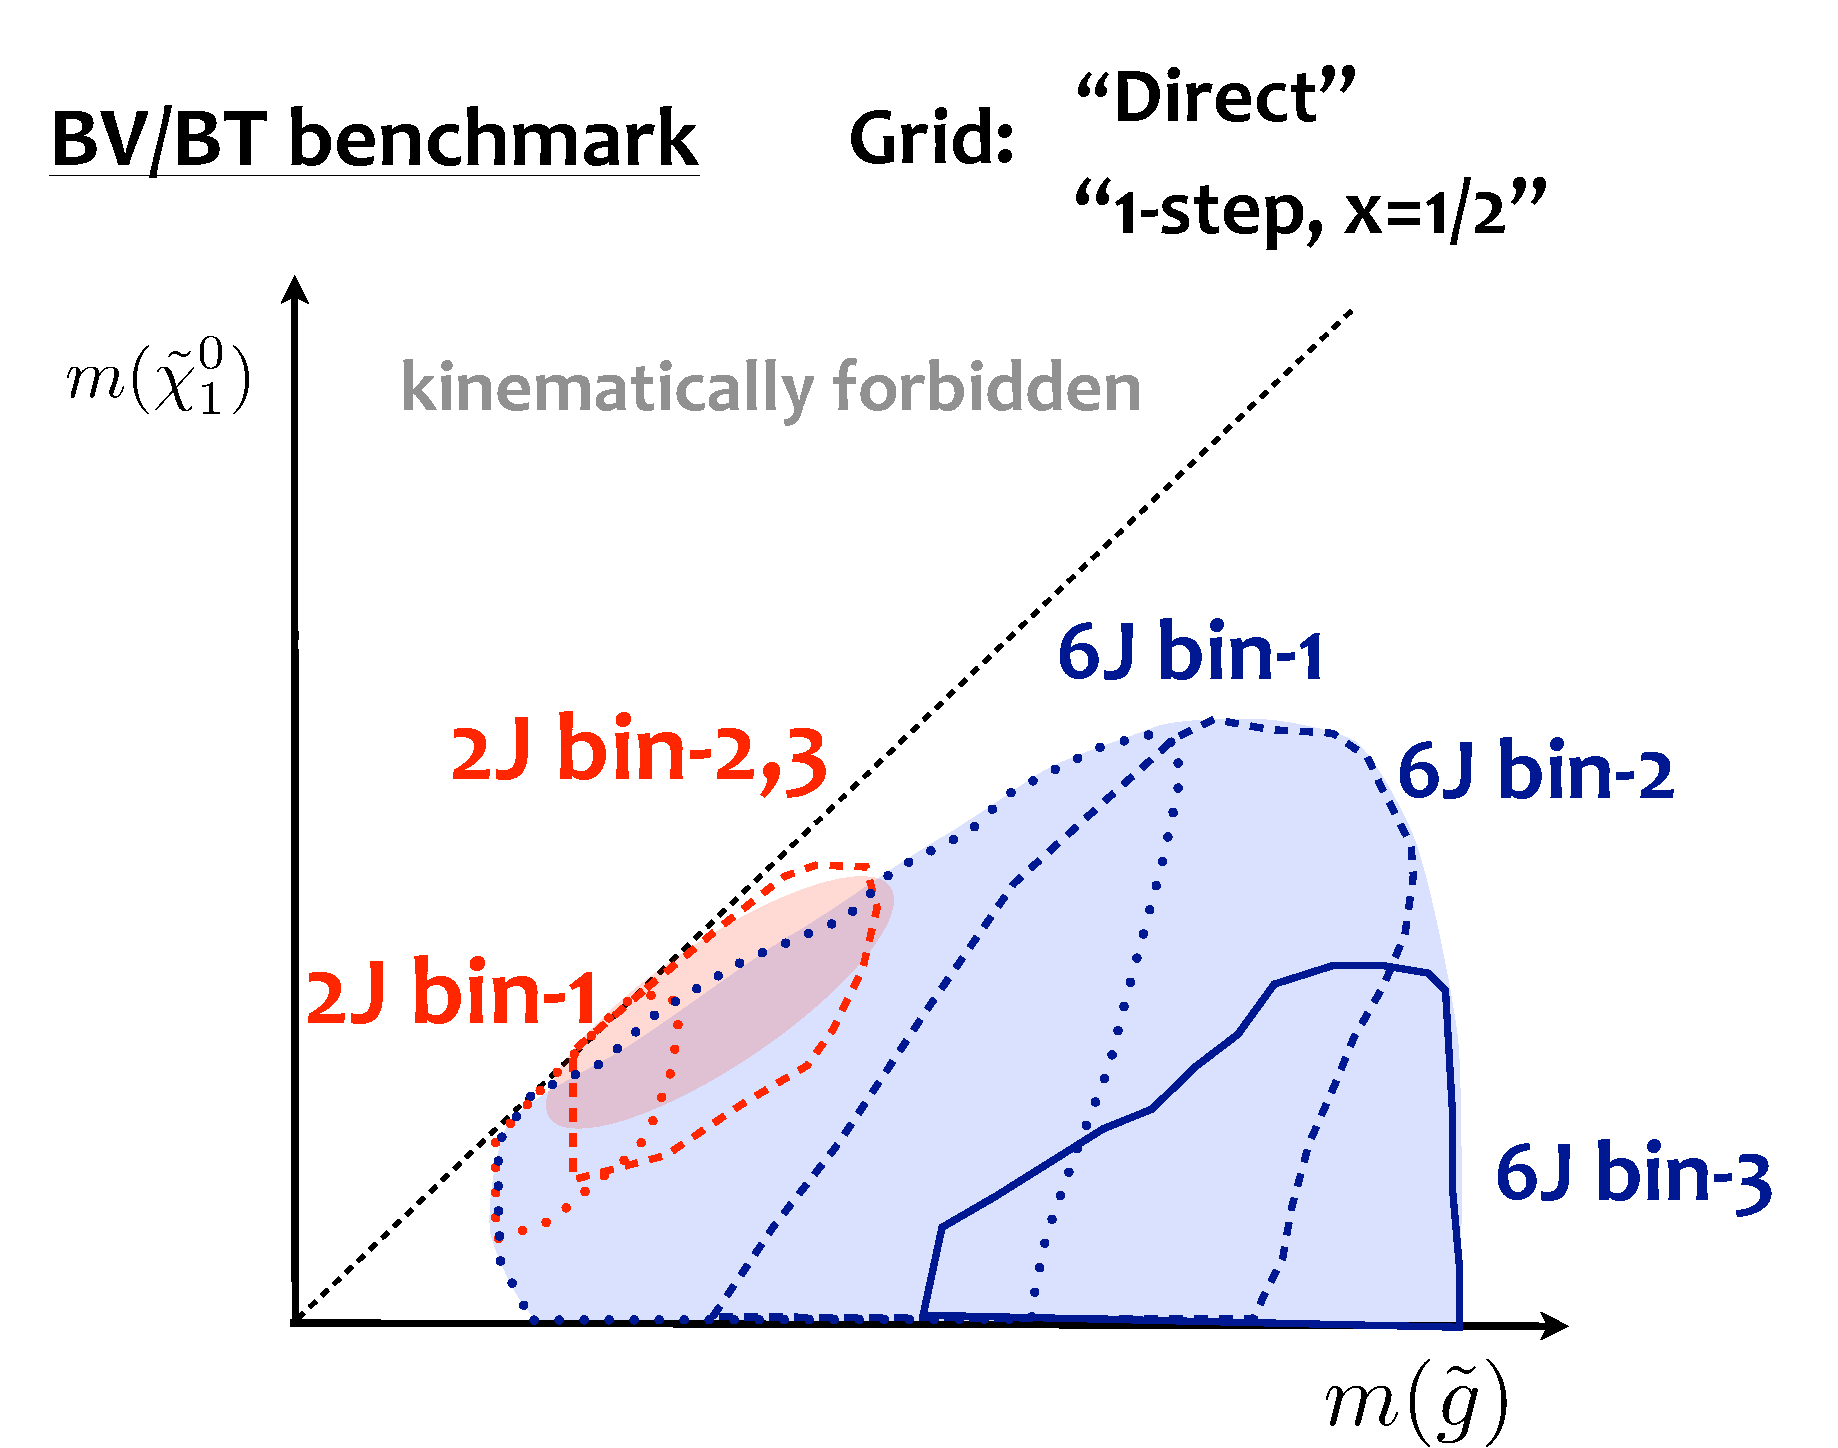
\includegraphics[width=0.7\textwidth]{figures/SRdefinition/EventSelection/TowerCoverage_BVBT_x12.pdf}}
    \subfigure[]{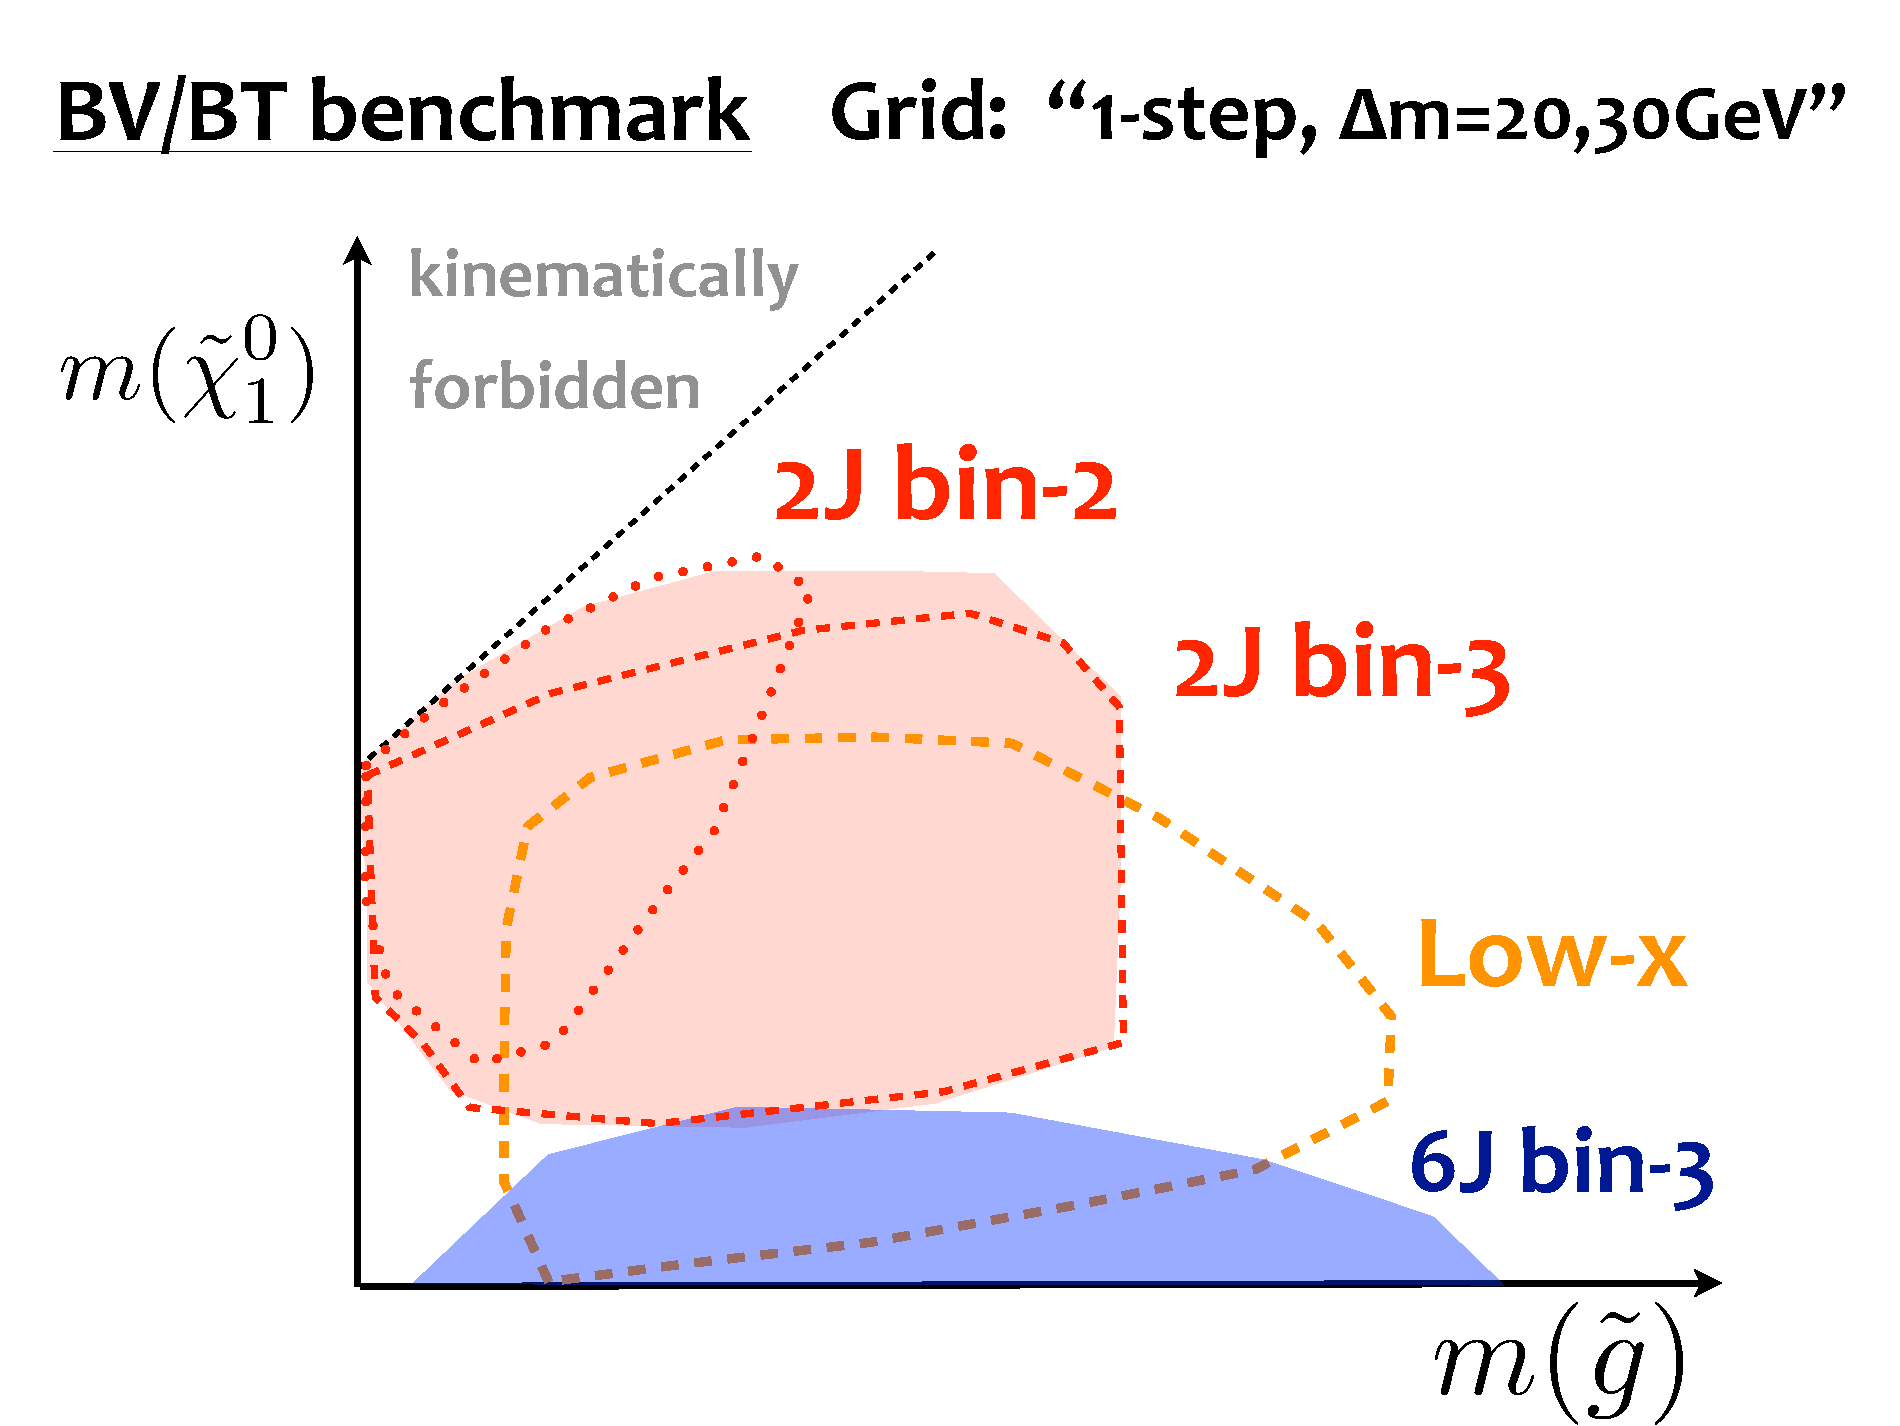
\includegraphics[width=0.7\textwidth]{figures/SRdefinition/EventSelection/TowerCoverage_BVBT_dM.pdf}}
    \caption{ 
     Sensitivity converage by individual signal region towers or $\meffInc$-bins in the 
    (a) the \dire and \xhalf grid, and in (b) the \DMtw, \DMth  grid of the BT/BV benchmark models. Dashed contours and shaded areas schematize the regions that the individual tower or $\meffInc$-bin addresses the sensitivity.}
    \label{fig::SRdefinition::towerCoverage1}
\end{figure}

\begin{figure}[h]
  \centering
    \subfigure[]{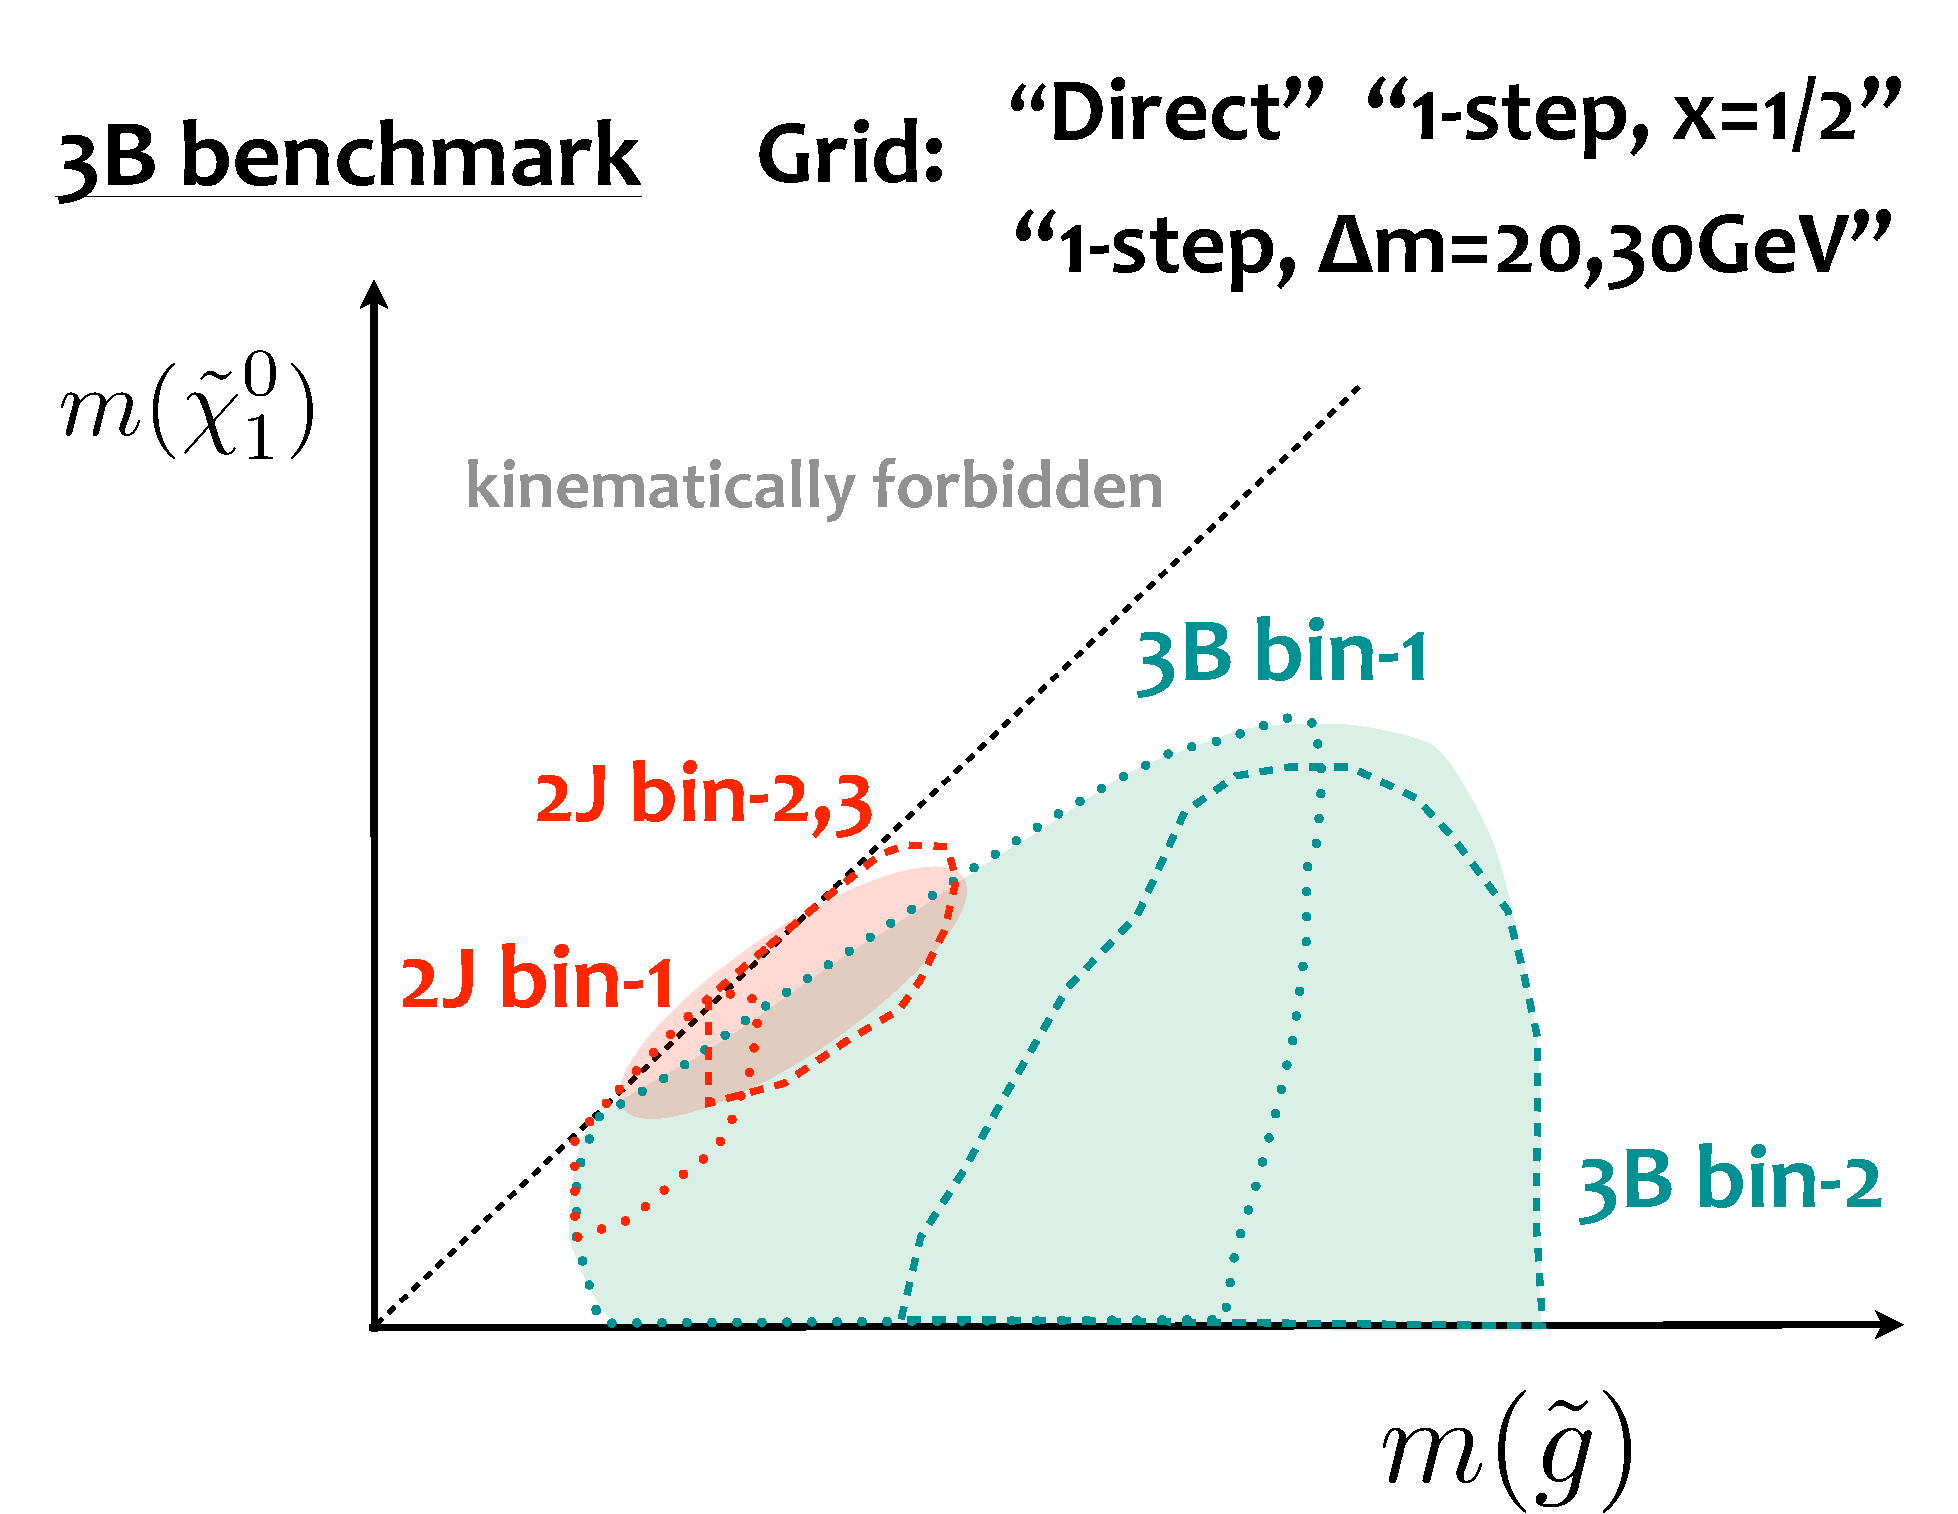
\includegraphics[width=0.6\textwidth]{figures/SRdefinition/EventSelection/TowerCoverage_3B_x12.pdf}}
    \subfigure[]{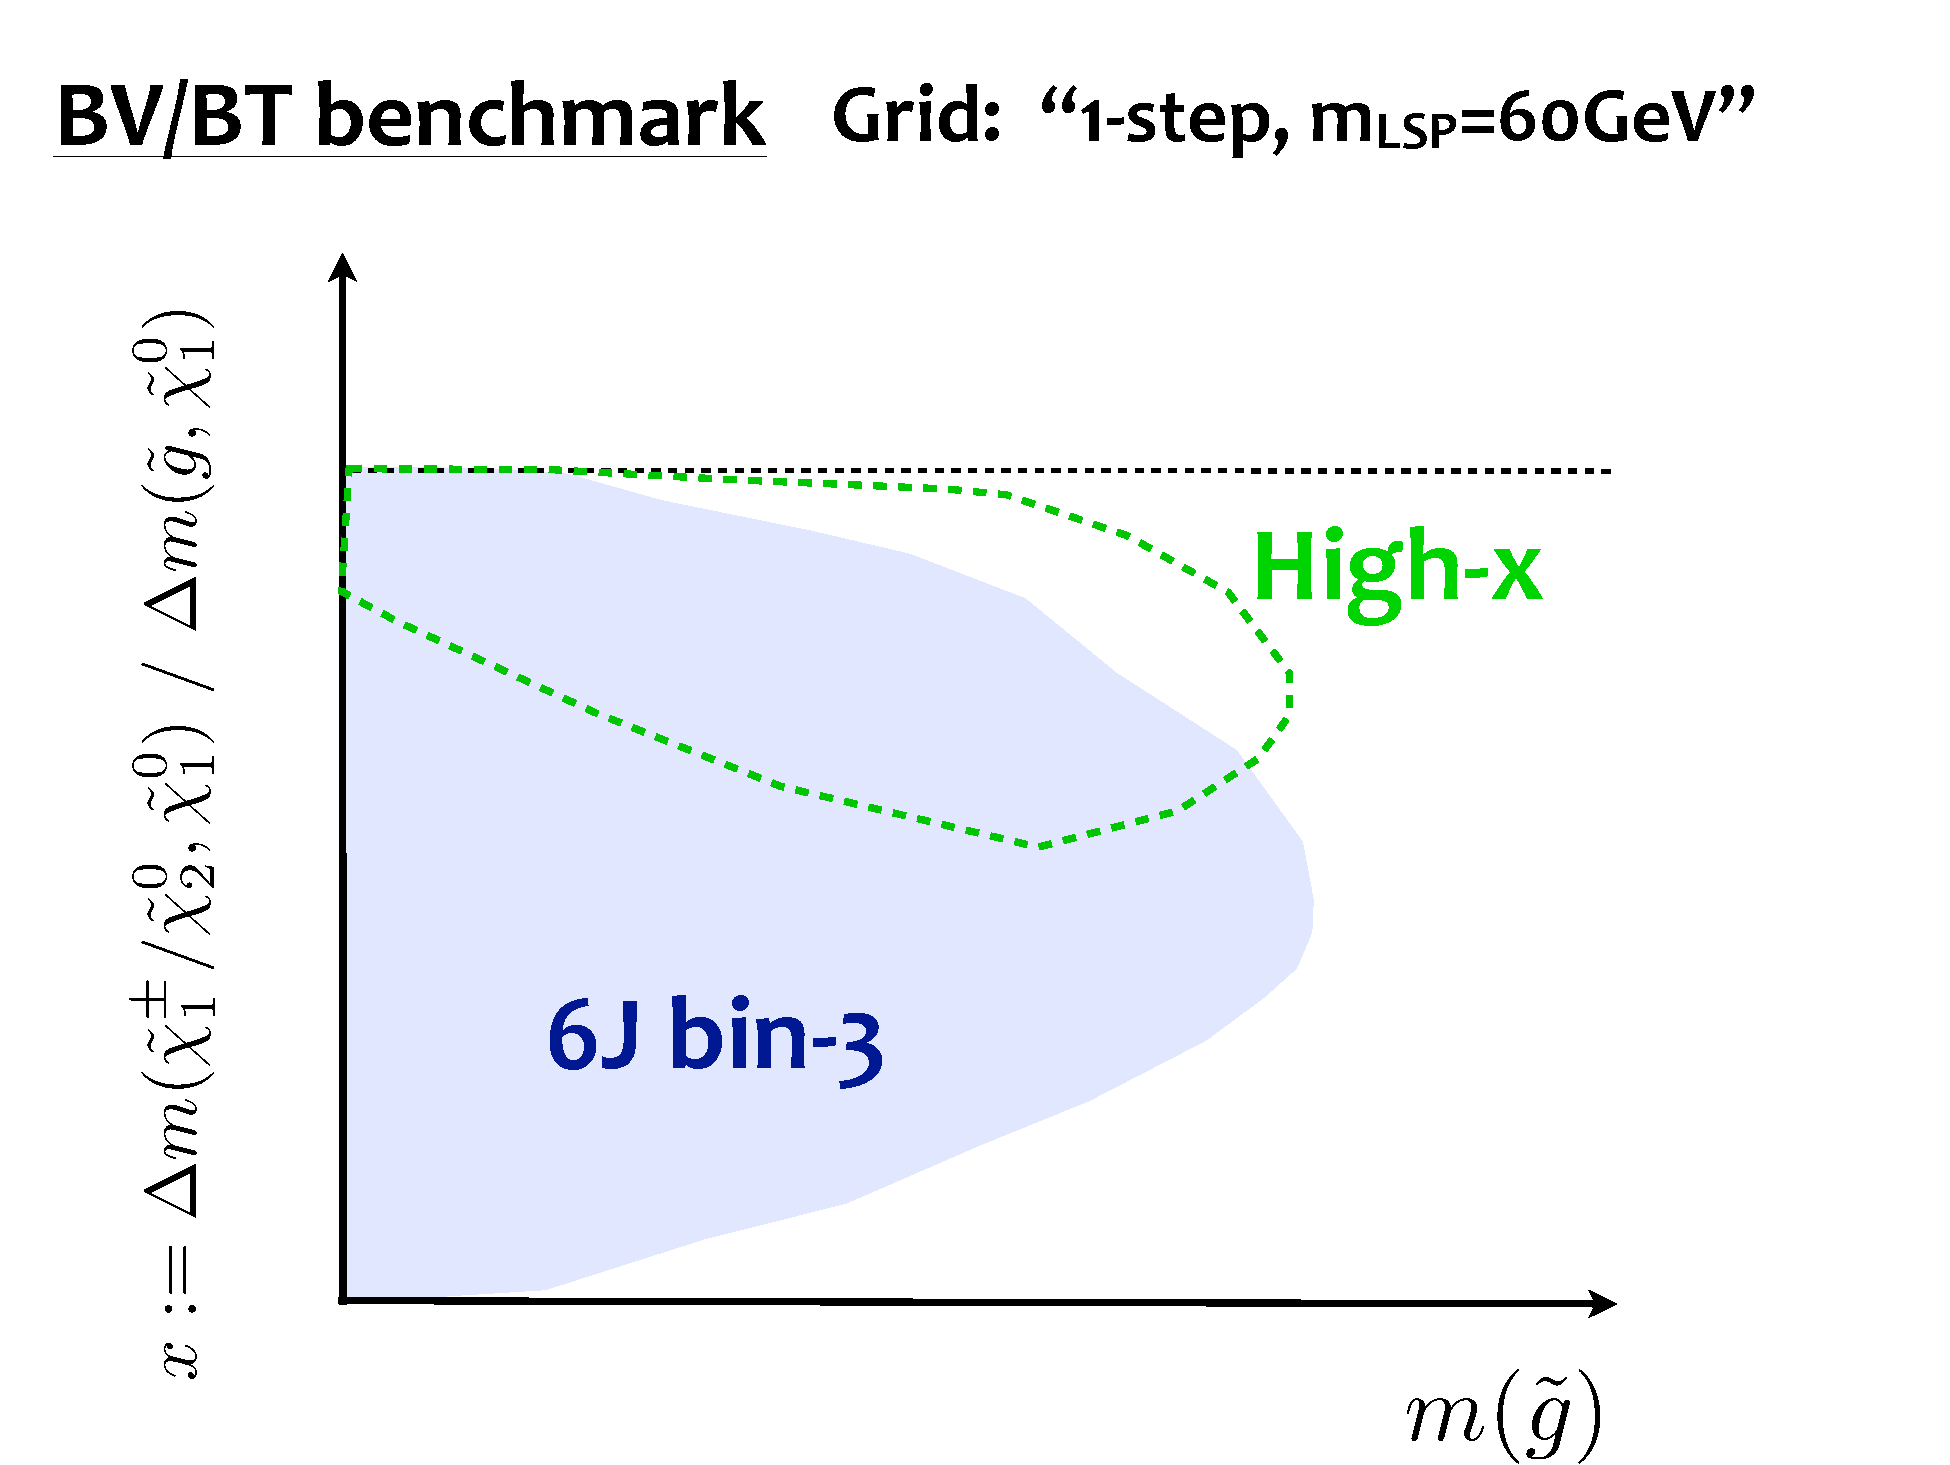
\includegraphics[width=0.5\textwidth]{figures/SRdefinition/EventSelection/TowerCoverage_BVBT_varx.pdf}}
    \subfigure[]{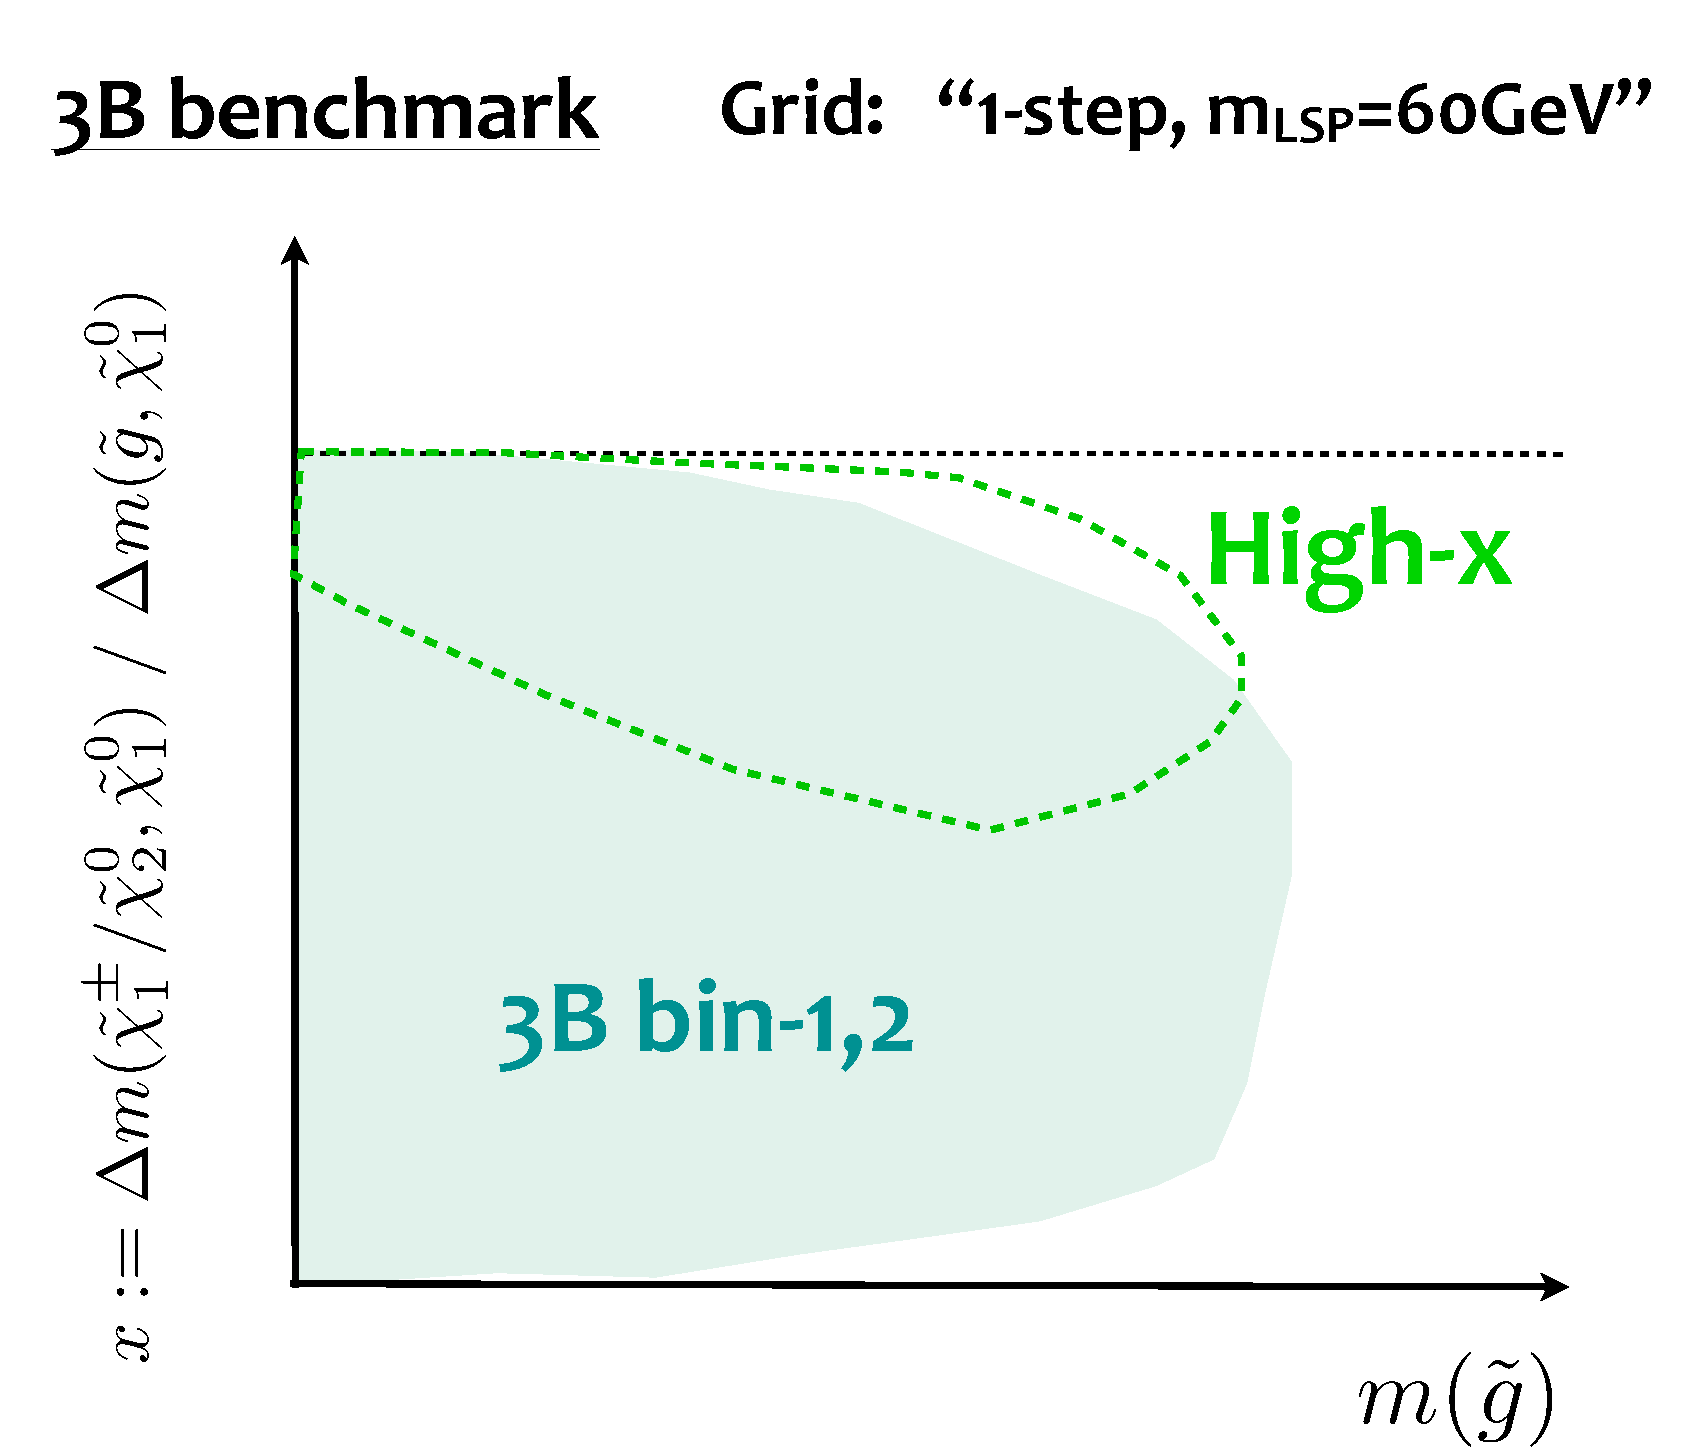
\includegraphics[width=0.45\textwidth]{figures/SRdefinition/EventSelection/TowerCoverage_3B_varx.pdf}}
    \caption{ 
     Sensitivity converage by individual signal region towers or $\meffInc$-bins in the 
    (a) \dire, \xhalf, \DMtw and \DMth grids of the 3B benchmark models, (b) the \varx grid of the of the BT/BV benchmark models, and in (c) the \varx grid of the 3B benchmark models. Dashed contours and shaded areas schematize the regions that the individual tower or $\meffInc$-bin addresses the sensitivity.}
    \label{fig::SRdefinition::towerCoverage2}
\end{figure}


\clearpage
% ------ Definition of Variables
\subsubsection{Discriminating variables}
Kinamtical variables used for background rejection as well as defining control regions are overviewed. The distributions of backgrounds overlaid with benchmark signals at the preselection are presented in Fig. \ref{fig::SRdefinition::distVar1} - \ref{fig::SRdefinition::distVar2}. In addition to the pre-selection, a soft lepton ($\pt(\ell)\in[6,35]$) is required in Fig. \ref{fig::SRdefinition::distVar2} (b), $\meffInc>1500\gev$ in for Fig. \ref{fig::SRdefinition::distVar2} (b), and $\nBJetNoGev \geq3 \,\,\, \mt>125\gev$ are applied in Fig. \ref{fig::SRdefinition::distVar2} (c) and (d). The definition and the purpose of the variables are as below: \\

\paragraph{${\bf \nJetNoGev}$}
Jet multiplicity often shows the great discriminating power since the standard model processes suffer a sharp cut-off.
However one should mind that the optimum cut is significantly dependent on the gluino decay mode, and also that the aggressive cut will enhance the contribution from higher order effect, putting the modeling at the risk of large theoretical uncertainty.
Therefore, it is kept to a moderated use as means of background rejection. \\

\paragraph{${\bf \met}$}
Signal events result in large $\met$ reflecting the presence of hard additional undetected LSP when $\dmg$ is large.
At analysis level, this is also true for the compressed case given that the MET via ISRs is nevertheless required for the trigger sake as described above.

\paragraph{${\bf \meffInc}$} 
$\meffInc$ is the variable best reflecting the magnitude of absolute mass splitting $\dmg$, providing the best separation against backgrounds.
Meanwhile it is also noticable that the magnitude of $\meffInc$ is almost uniquely determined by $\dmg$, regardless of the relative mass splitting and gluino decays, 
therefore the optimal cut in $\meffInc$ is highly universal.
%better than applying cuts on jet pt individually giving the low xsec for signal that cant afford in acceptance.


\paragraph{${\bf \mtFull}$} 
Invariant mass of $\met$ and the lepton with the z-momentum set to 0.
Analogous to ordinary invariant mass peaking at the mass of the parent particle, the end point of $\mt$ represents the parent mass when they share the same origin.
Since SM 1-lepton process is always with a leptonically decaying W-boson without additional hard missing particles, the bulk component experiences a sharp cut-off in $\mt$ around $m_W = 81.4 \gev$, 
therefore the cut above $m_W$ is tremendously effective.


\paragraph{${\bf \met/\meffInc}$}
$\met/\meffInc$ separates backgrounds and signals targeted by the \textbf{2J} and \textbf{High-x} where jet activity is relatively low compared with the magnitude of MET required.


\paragraph{Aplanarity}
Aplanarity is a variable characterizing the 3-dimensionality of an event in terms of the final state particles. It is defined as the thirtial eigenvalue of the normalized jet momentum tensor $S$:
\begin{align}
  S^{\alpha \beta} & := \frac{\sum_i p_i^{\alpha} p_i^{\beta} }{\sum_i |\bm{p_i}|^2 }, \nn \\ 
  %
  P^{-1}SP & = \left(
  \begin{array}{c c c }
    \lambda_1  & & \\
    & \lambda_2 & \\
    & & \lambda_3 \\
  \end{array}
  \right), \,\,\, \lambda_1 > \lambda_2 > \lambda_3, \nn \\
  \mathrm{Aplanarity} & := \frac {3}{2} \times \lambda_3,
  %
\end{align}
where $P$ stands for the $3\times3$ matrix diagonalizing $S$, $\lambda_i$ for the eigenvalues of $S$.
It ranges from $0<A<1/2$; $A=0$ corresponds to events with jets distributed in the common plain, and $A=0.5$ represents the isotropically distributed event topology.
Aplanarity is an effective discriminator after requiring tight selection in $\meffInc$ or $\met$, where the remnant SM events (particularly $\wjets$) are typically heavily kicked by hard ISR radiations, leading to a highly linear event topology in their center-of-mass frame. These events end up in a planar topology in the lab frame once getting boosted toward the beam direction, as a result populating in low aplanarity region accordingly. 
On the other hand, the decay of gluino pairs keep relatively spherical thus the aplanarity distributing rather flatly, which reflects the fact the gluinos are too heavy to be boosted.


\paragraph{${\bf \nJetNoGev/\lepOnePt}$}
Since the hardness of lepton and jets are positively correlated in normal processes in SM, it is relatively rare to end up in a soft lepton and hard jet activity simultaneously, while it is the case for the compressed gluino signature. A variable $\nJetNoGev/\lepOnePt$ helps visualize the different correlations, and used in the \textbf{2J} signal region towers to improve the sensitivity of the compressed gluino signatures.


\paragraph{${\bf \mindPhiFourJet}$}
vA variable indended to reject the remnant $\ttbar$ events after requiring tight selection of $\meffInc$ and $\met$. 
As such $\ttbar$ events typically have hard ISR jets to boost the $\ttbar$ system, the jets from $\ttbar$ decays and associated soft radiation tend to be collimated each other. Conversely, the jets from the gluino decays almost never get collimated as due to the heavy mass of gluino.


\paragraph{Topness}
One of the most important background in 1-lepton analysis is di-leptonic $\ttbar$ events with a hadronically decaying tau lepton or a lepton that fails the baseline requirement. To reject those events, a $\chi^2$-based di-leptonic $\ttbar$ tagger ``topness'' has been designed in context of scalar-top search since Run1 \cite{Topness}. 
The $\chi^2$ function is defined as:
\begin{align}
& S(p_{\mathrm{W}}^x, p_{\mathrm{W}}^y, p_{\mathrm{W}}^z, p_{\nu}^z)  \nn  \\
& = \chi^2(m_{t,1}^2) + \chi^2(m_{t,2}^2) + \chi^2(m_{W,1}^2) + \chi^2(\hat{s}(\ttbar))  \nn  \\
& = \frac{  \left( m_t^2 - (p_{b,1}+p_{\ell}+p_{\nu})^2                      \right)^2   }{a_t^4}  \nn \\
& + \frac{  \left( m_t^2 - (p_{b,2}+p_\mathrm{W})^2                          \right)^2   }{a_t^4}  \nn  \\
& + \frac{  \left( m_\mathrm{W}^2 - (p_{\ell}+p_{\nu})^2                     \right)^2   }{a_\mathrm{W}^4}  \nn \\
& + \frac{  \left( 4m_t^2- (p_{\ell}+p_{\nu}+p_{b,1}+p_{b,2}+p_\mathrm{W})^2 \right)^2   }{a_{\ttbar}^4},
\label{eq:SRdefinition::topness}
\end{align}
assuming an event topology as shown Fig. \ref{fig::SRdefinition::topness_diagram} where one of the lepton are totally undetected and the momentum does fully contribute to MET. \\
It consists of four gaussian constraints imposing the mass constraint of top-quark and W-boson, and the center-of-mass for the $\ttbar$ system being close to its minimum threshold ($2m_t$). The width parameters are set to $(a_t, a_W, a_{\ttbar})=(15,5,1000) \gev$, accounting for the Breit-Wigner widths of top-quark and W-boson as well as the tail of $\hat{s}(\ttbar)$ distribution. Although there are three missing particles in the topology, the number of unknown degree of freedom can be reduced into 4 by combining the missing lepton ($\ell_2$) and the paired neutrino ($\nu'$) into a single onshell W-boson and imposing the vectoral sum of transverse momenta of missing particles being equal to $\met$. 
Topness is then defined as the minimum $\chi^2$ when scanning over the four DOFs parametrized by $\bm{p}_{\mathrm{W}}$ and $p_{\nu}^z$:
\begin{align}
\mathrm{Topness} := \min_{p_{\mathrm{W}}^x, p_{\mathrm{W}}^y, p_{\mathrm{W}}^z, p_{\nu}^z} \ln[S].
\end{align}
Events in the topology assumed are supposed to have solutions ($p_{\mathrm{W}}^x, p_{\mathrm{W}}^y, p_{\mathrm{W}}^z, p_{\nu}^z$) that satisfy the four constraints at the same time while scanning, however it is not necessarily the case for the other type of events. Fig. \ref{fig::SRdefinition::topness_diagram} shows typical separation between di-leptonic $\ttbar$ and signals. Although di-leptonic $\ttbar$ does have a fraction of unfortunate events on the pile of higher values due to the fact that the energy of missing leptons or tau leptons does not entirely contribute to MET, the majority resides on the left pile while signals typically populate  more in the opposite one. 

%%%%%%%%% diagram for illustrating topness 
\fig[100]{SRdefinition/EventSelection/topness_diagram.pdf}
{Di-leptonic $\ttbar$ topology assumed in the topness calculation where one lepton is tagged ($\ell_1$) and the other lepton ($\ell_2$) is not identified as any objects with its momentum fully contributing to MET. Topness is defined as minimum summed $\chi^2$ of three mass shell constraints for the top, anti-top and the W-boson decaying into $\ell_1$, as well as one pseudo-mass constraint in terms of the $\ttbar$ systems (labeled as pink circles), while scanning over the momenta space of missing particles. The degrees of freedom by $\ell_2$ and the associated neutrino ($\nu_2$) are combined into a 4-momentum $p_W$ with the mass fixed to $m_W = 81.2\gev$, and the scan is performed in terms of $p_{\mathrm{W}}^x, p_{\mathrm{W}}^y, p_{\mathrm{W}}^z$ and $p_{\nu}^z$ from $-4\tev$ to $4\tev$ respectively.}
{fig::SRdefinition::topness_diagram}
%%%%%%%%%%%

\begin{figure}[h]
  \centering
    \subfigure[]{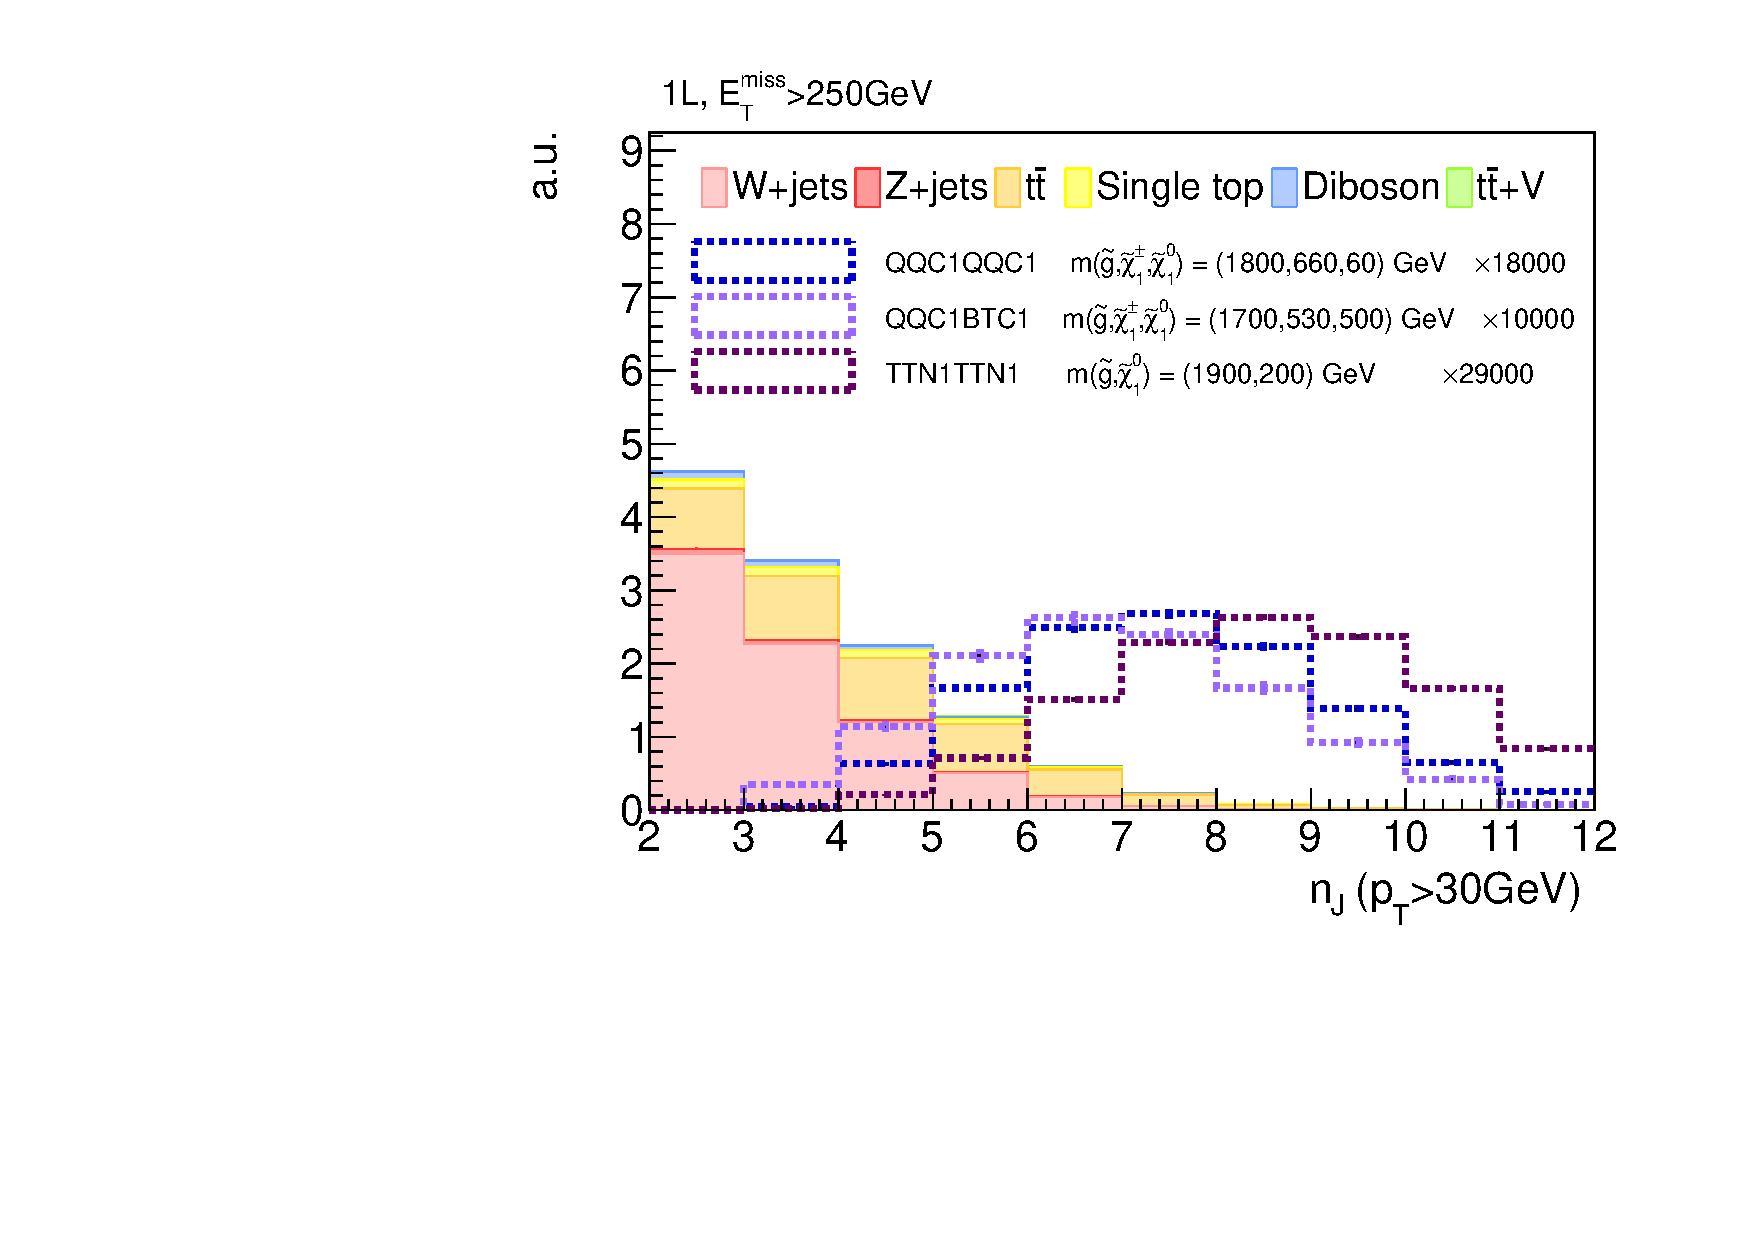
\includegraphics[width=0.48\textwidth]{figures/SRdefinition/discVar/nJet30__Precut.pdf}}
    \subfigure[]{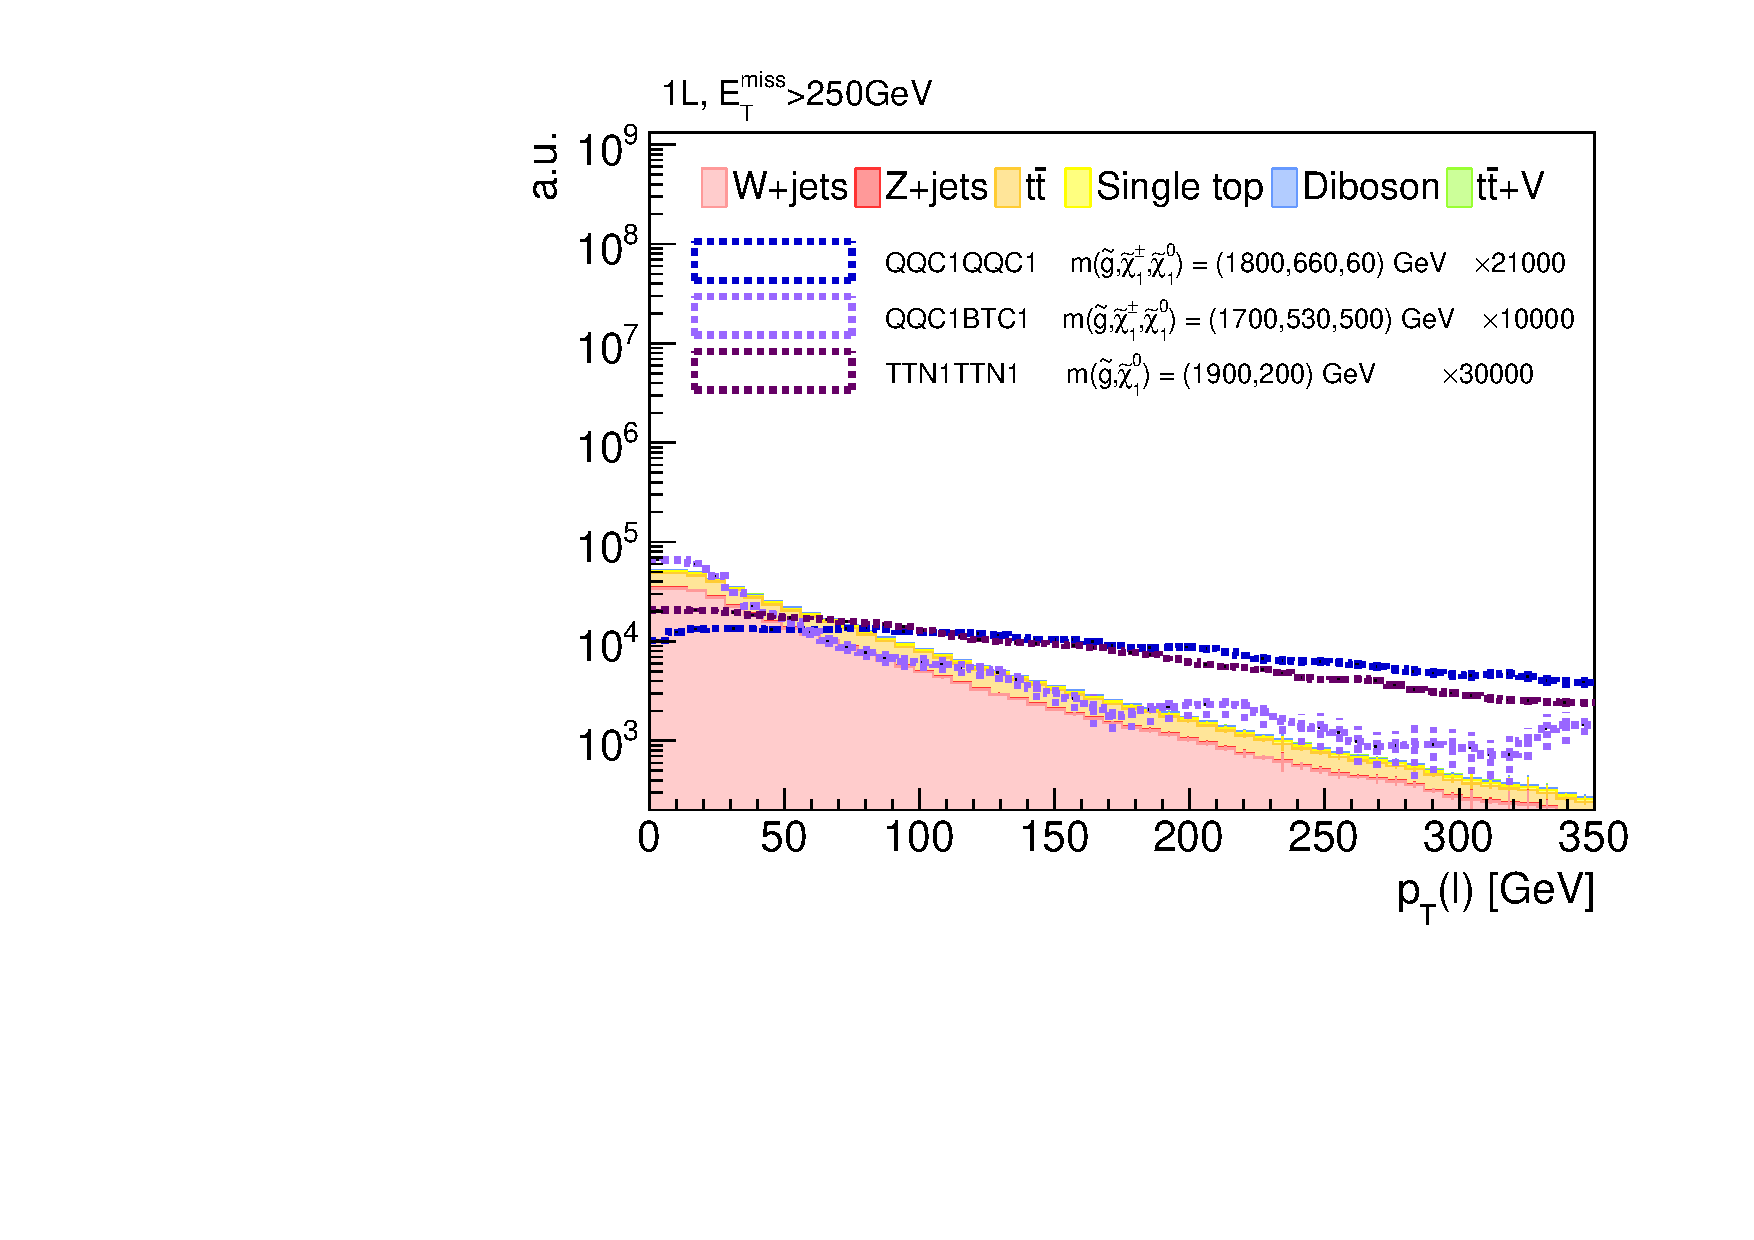
\includegraphics[width=0.48\textwidth]{figures/SRdefinition/discVar/lep1Pt__Precut_log.pdf}}
    \subfigure[]{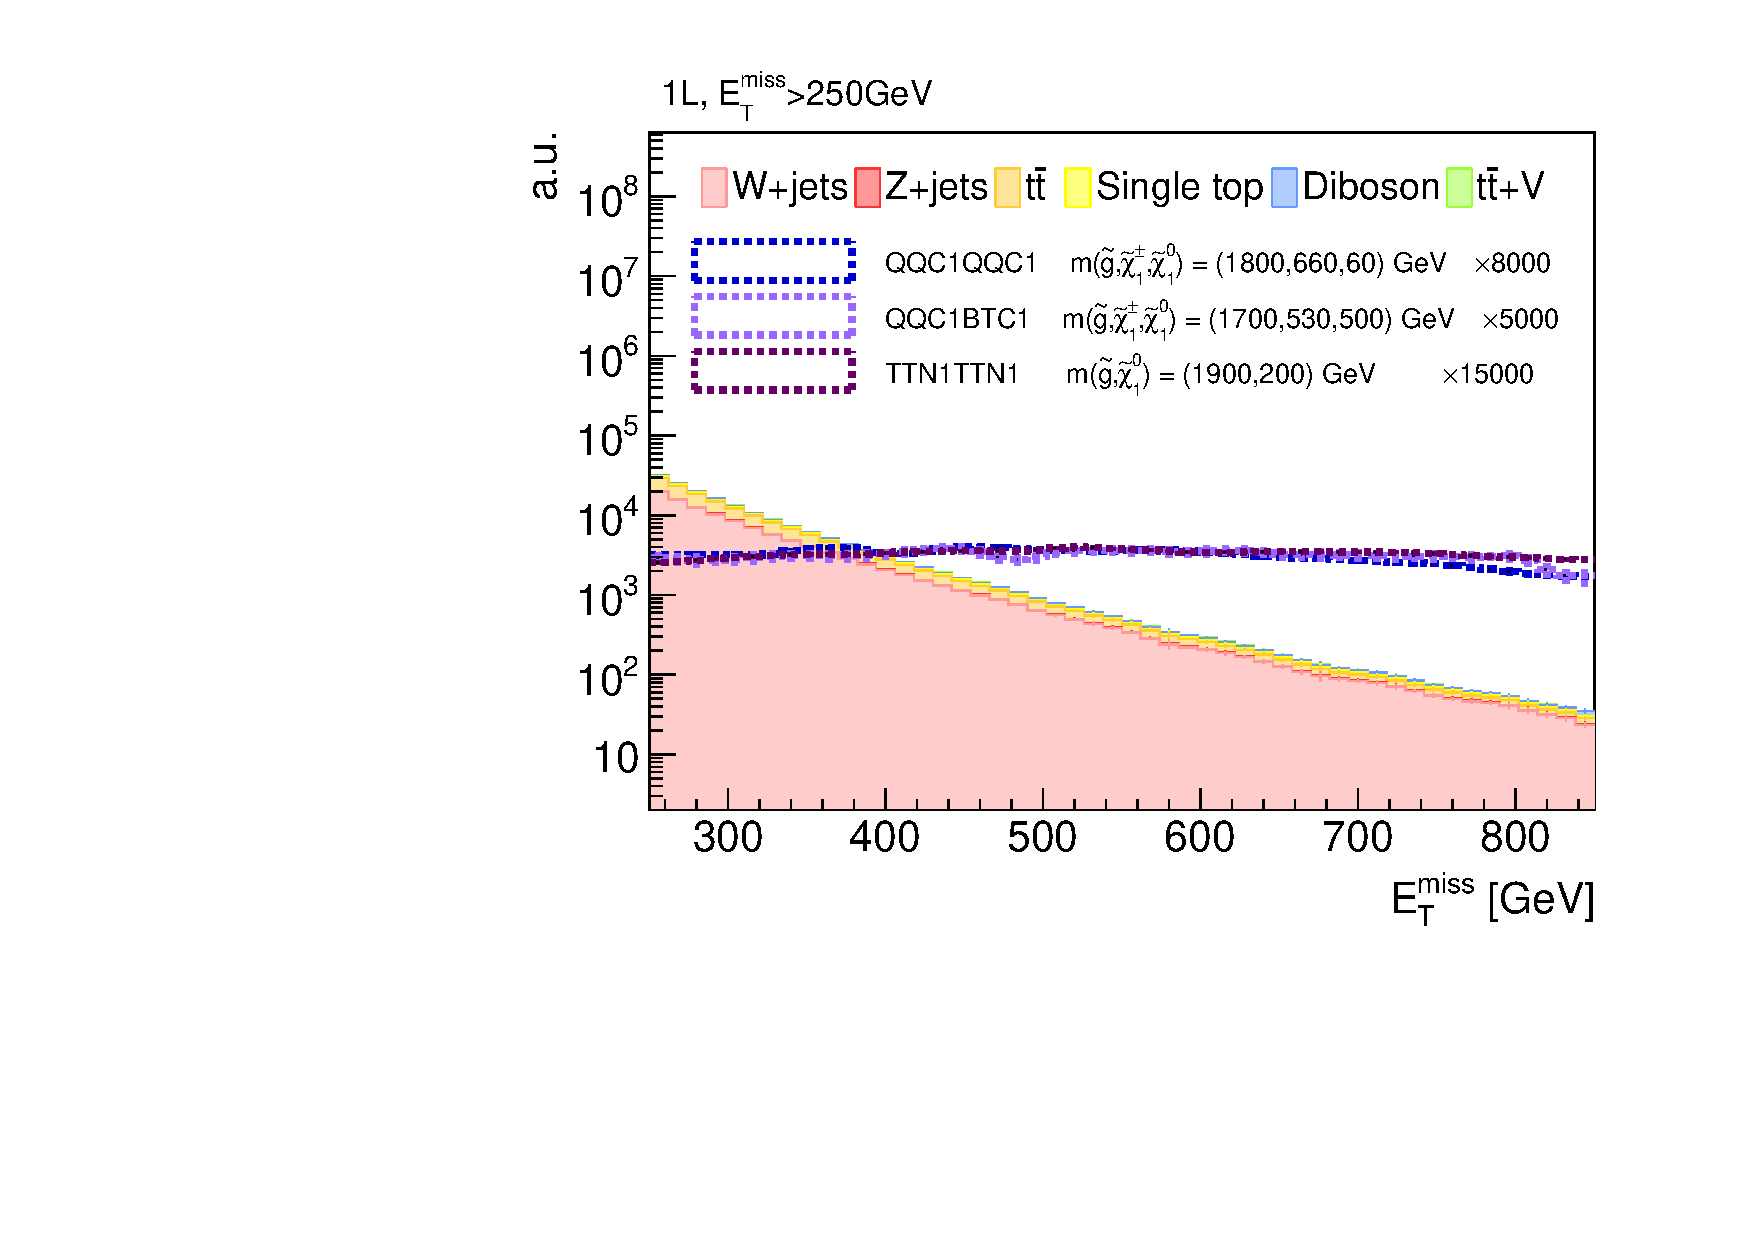
\includegraphics[width=0.48\textwidth]{figures/SRdefinition/discVar/met__Precut_log.pdf}}
    \subfigure[]{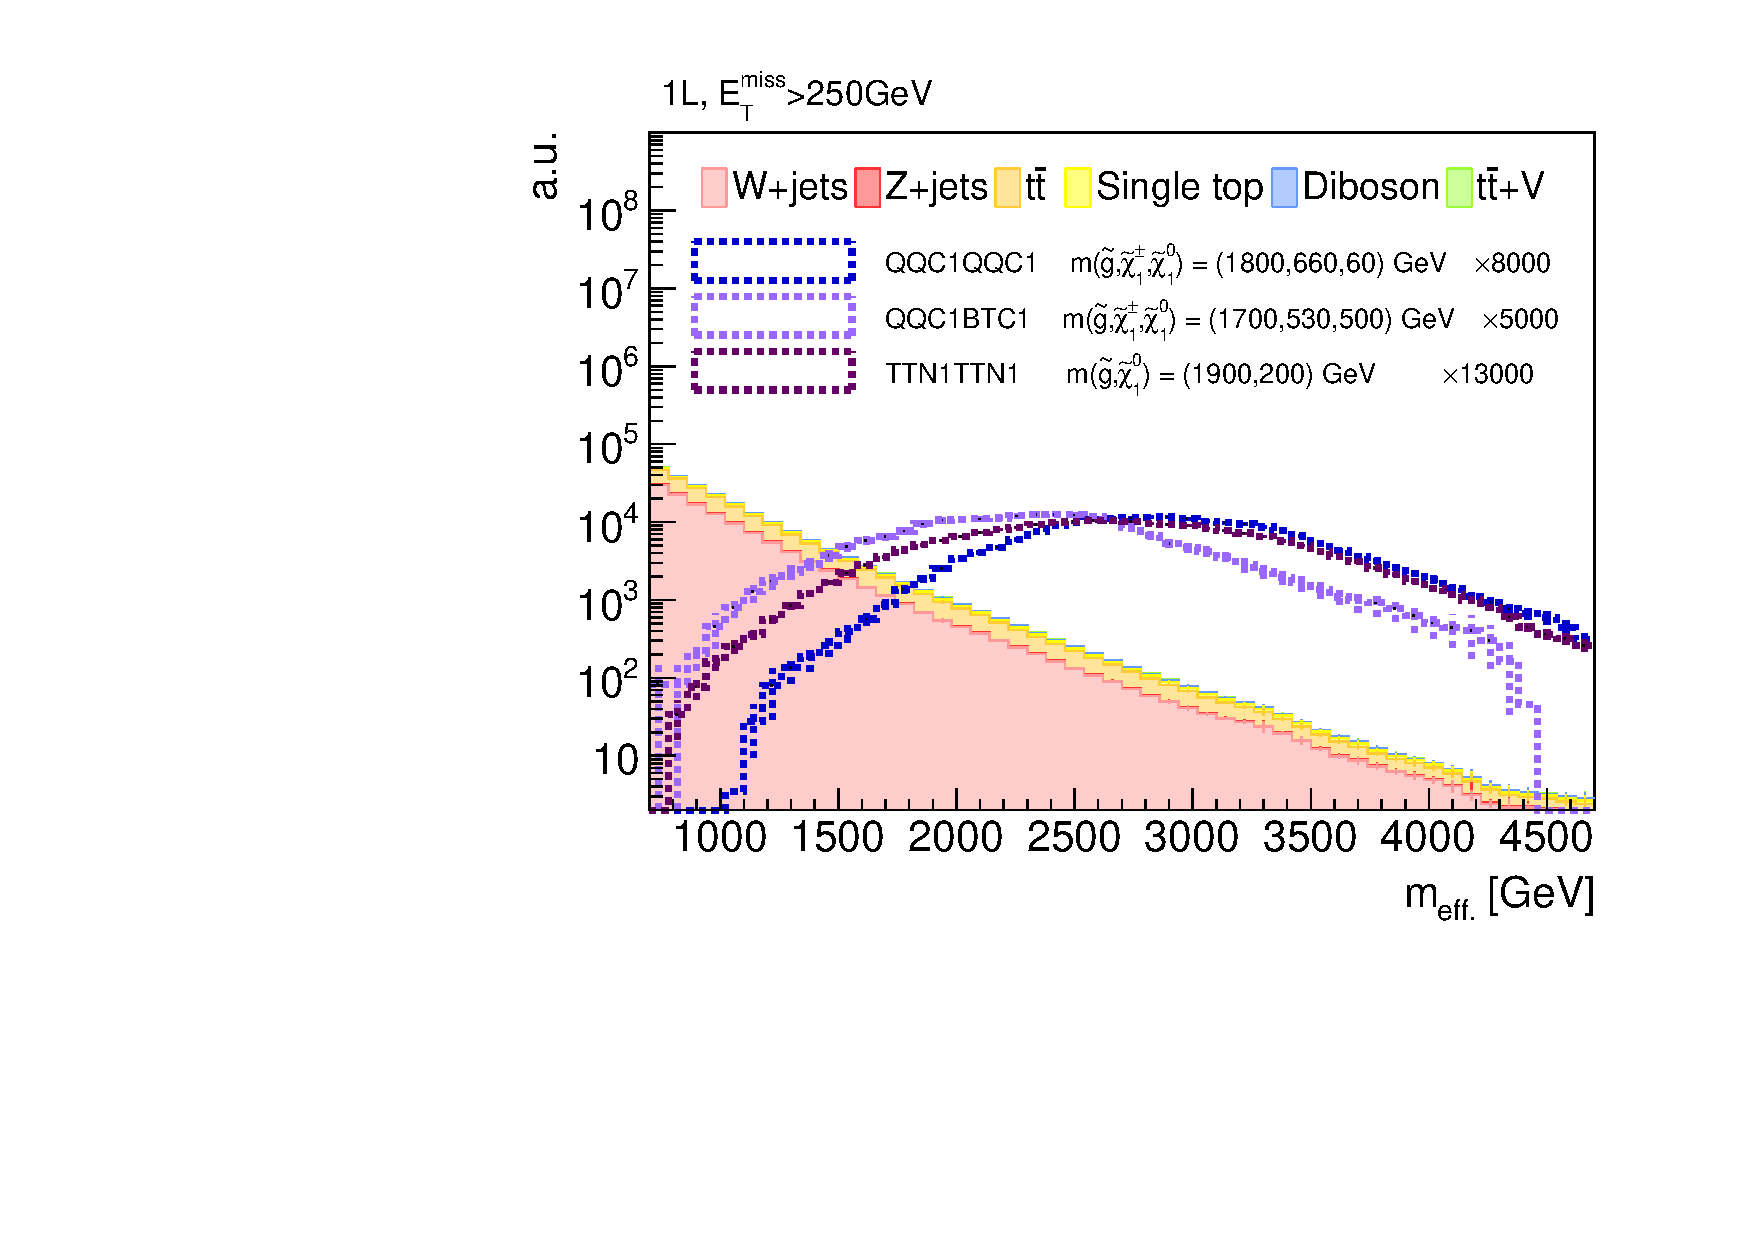
\includegraphics[width=0.48\textwidth]{figures/SRdefinition/discVar/meffInc30__Precut_log.pdf}}
    \subfigure[]{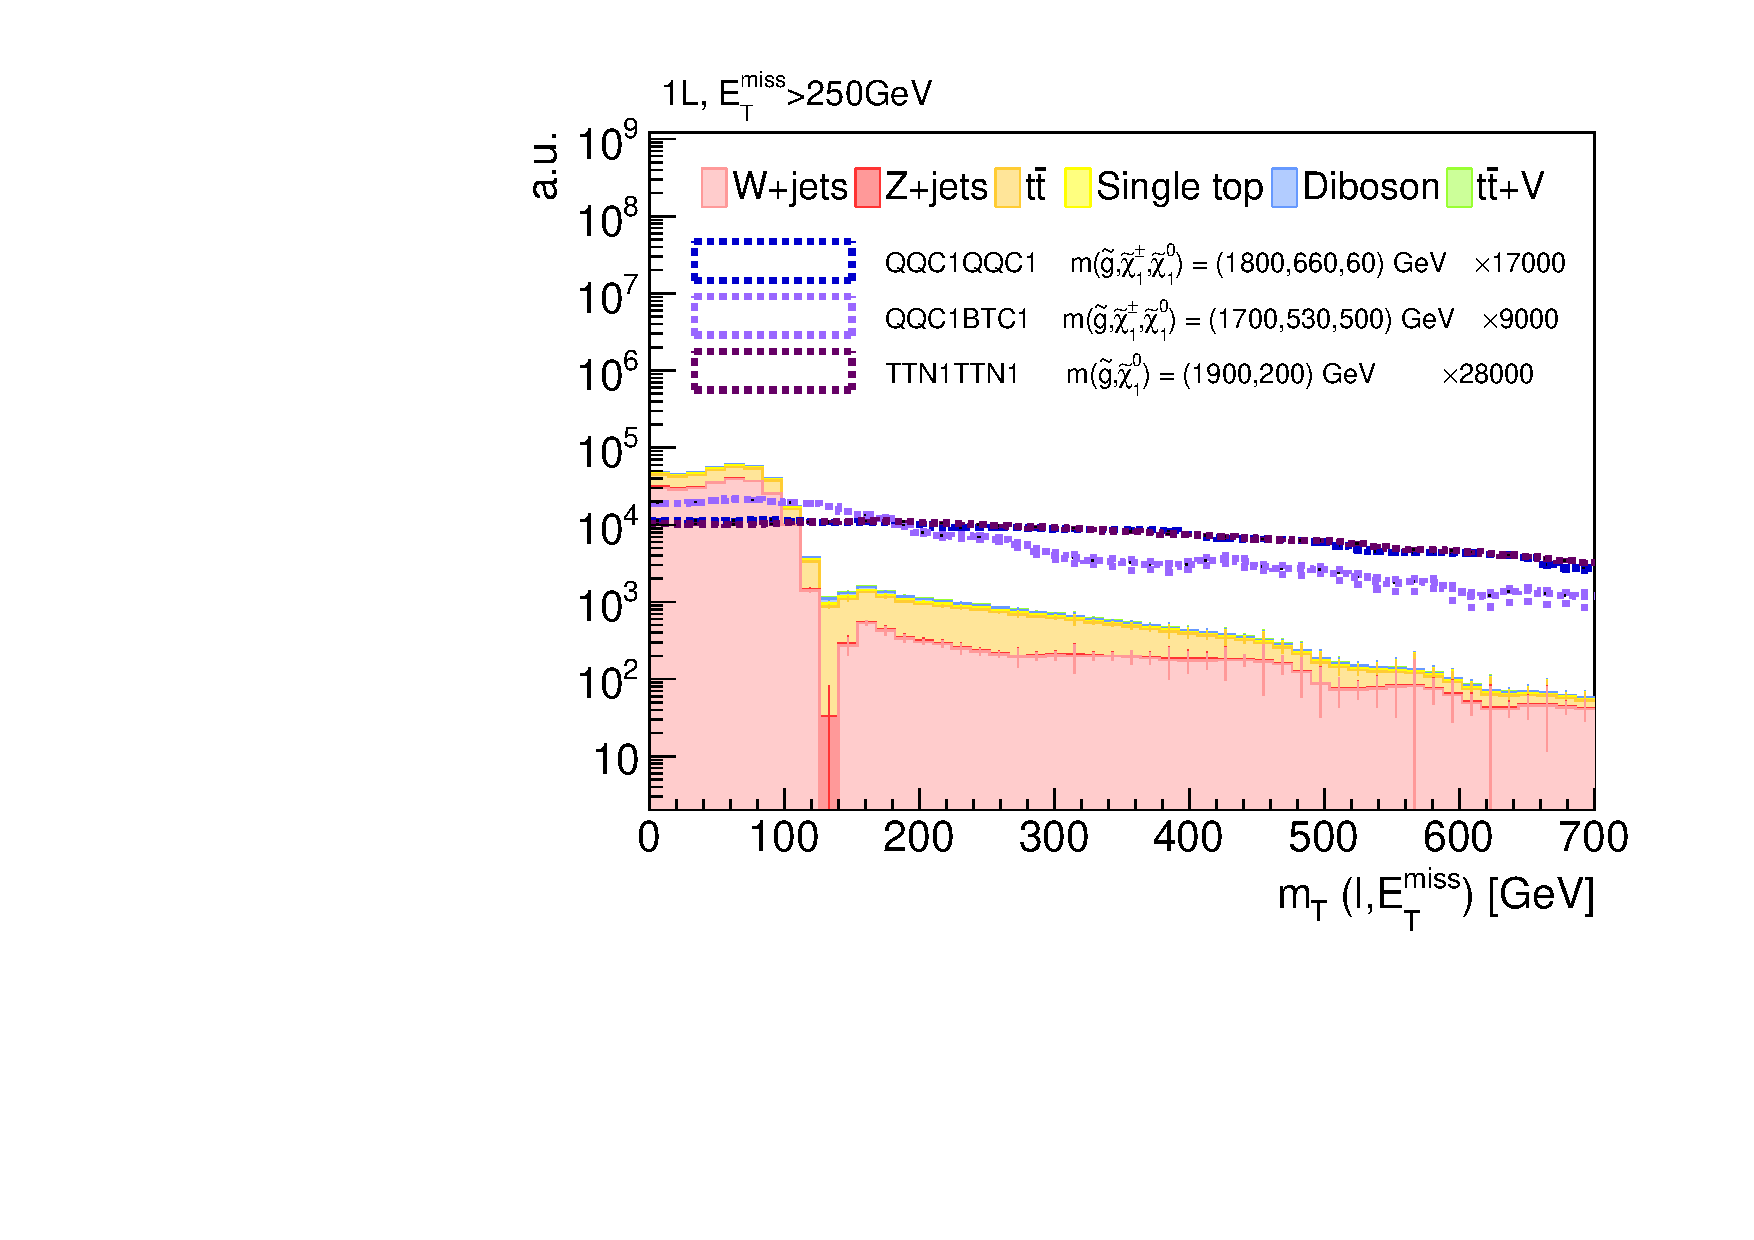
\includegraphics[width=0.48\textwidth]{figures/SRdefinition/discVar/mt__Precut_log.pdf}}
    \subfigure[]{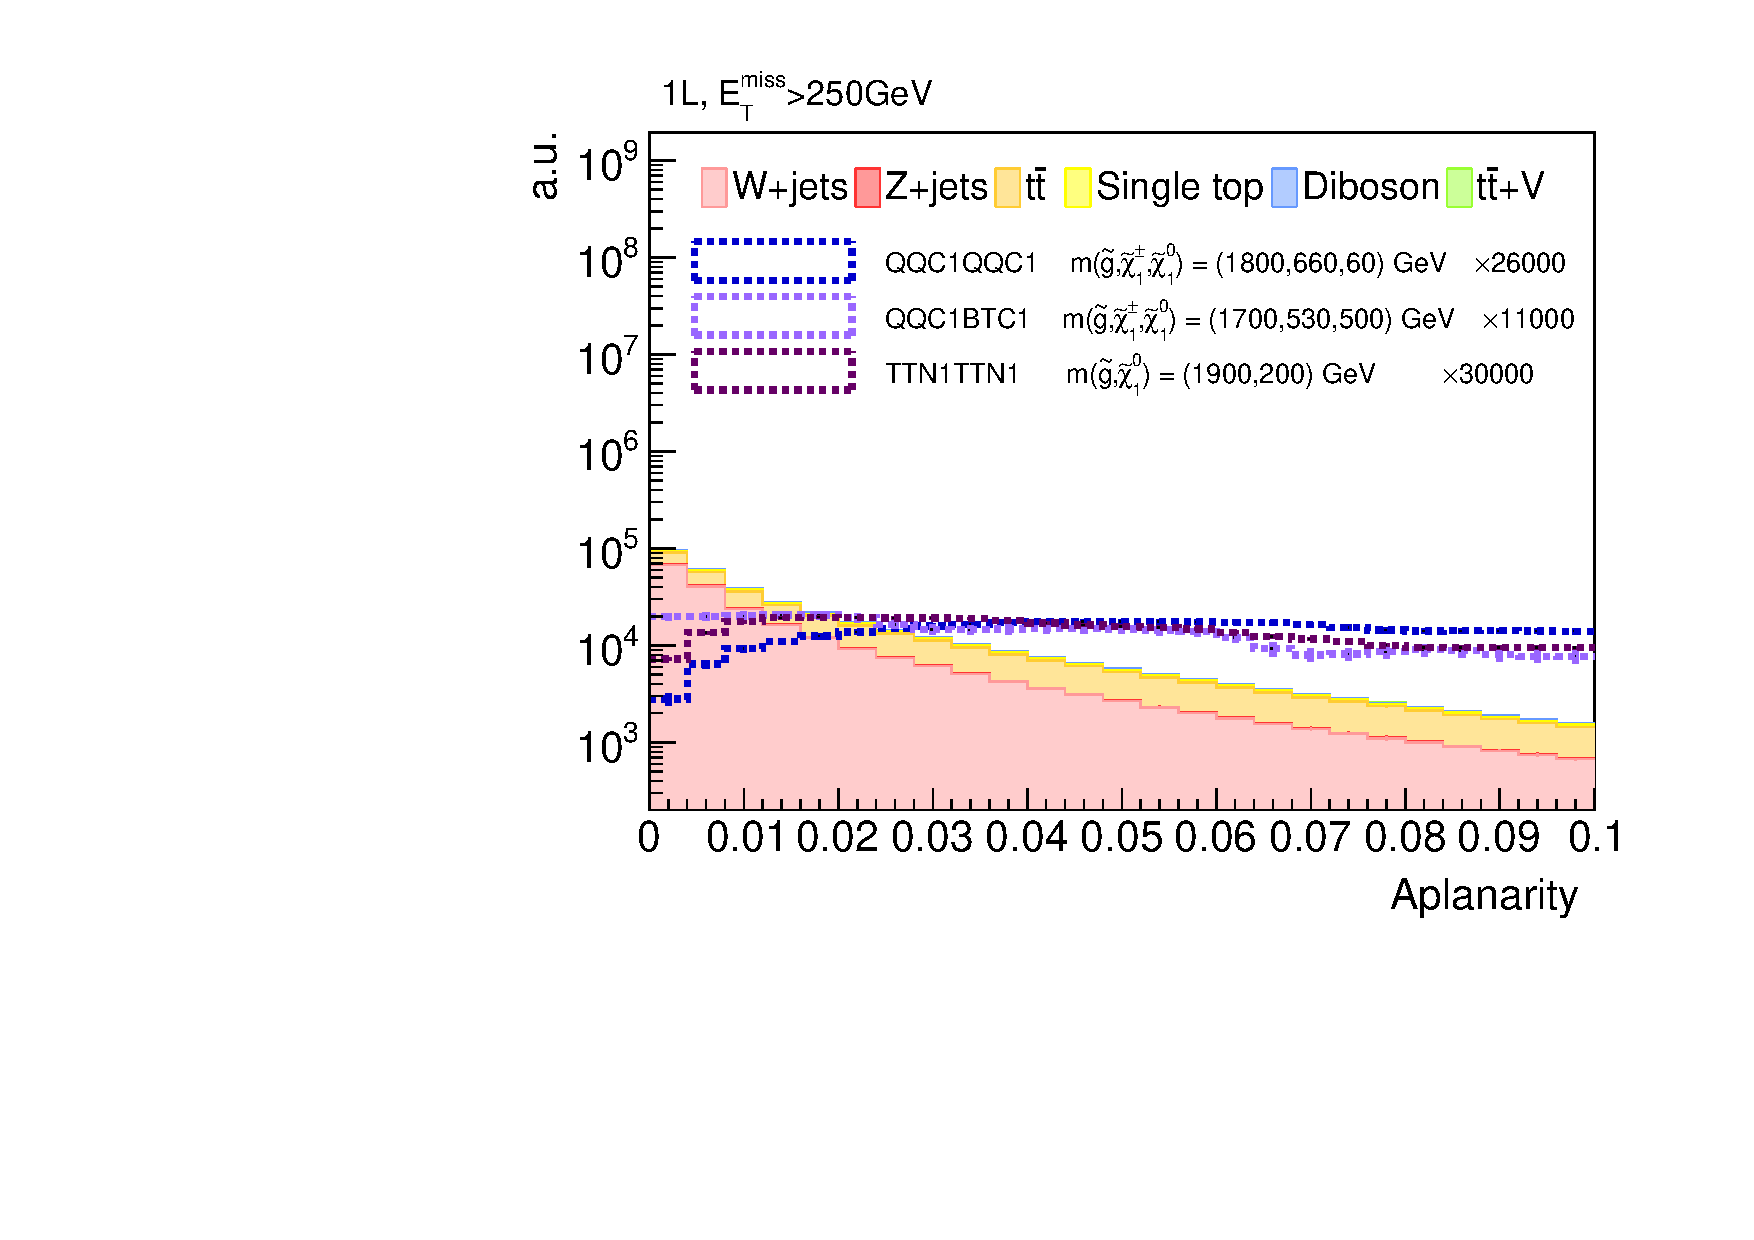
\includegraphics[width=0.48\textwidth]{figures/SRdefinition/discVar/LepAplanarity__Precut_log.pdf}}
    \caption{ 
    Distributions of discriminating variables for reference signal and backgrous, at the preselection level.
    (a) $n_J$, (b) Lepton $\pt$, (c) $\met$, (d) $\meffInc$, (e) $\mt$ and (f) aplanarity are respectively shown.
    \label{fig::SRdefinition::distVar1}       
    }
\end{figure}

\begin{figure}[h]
  \centering
    \subfigure[]{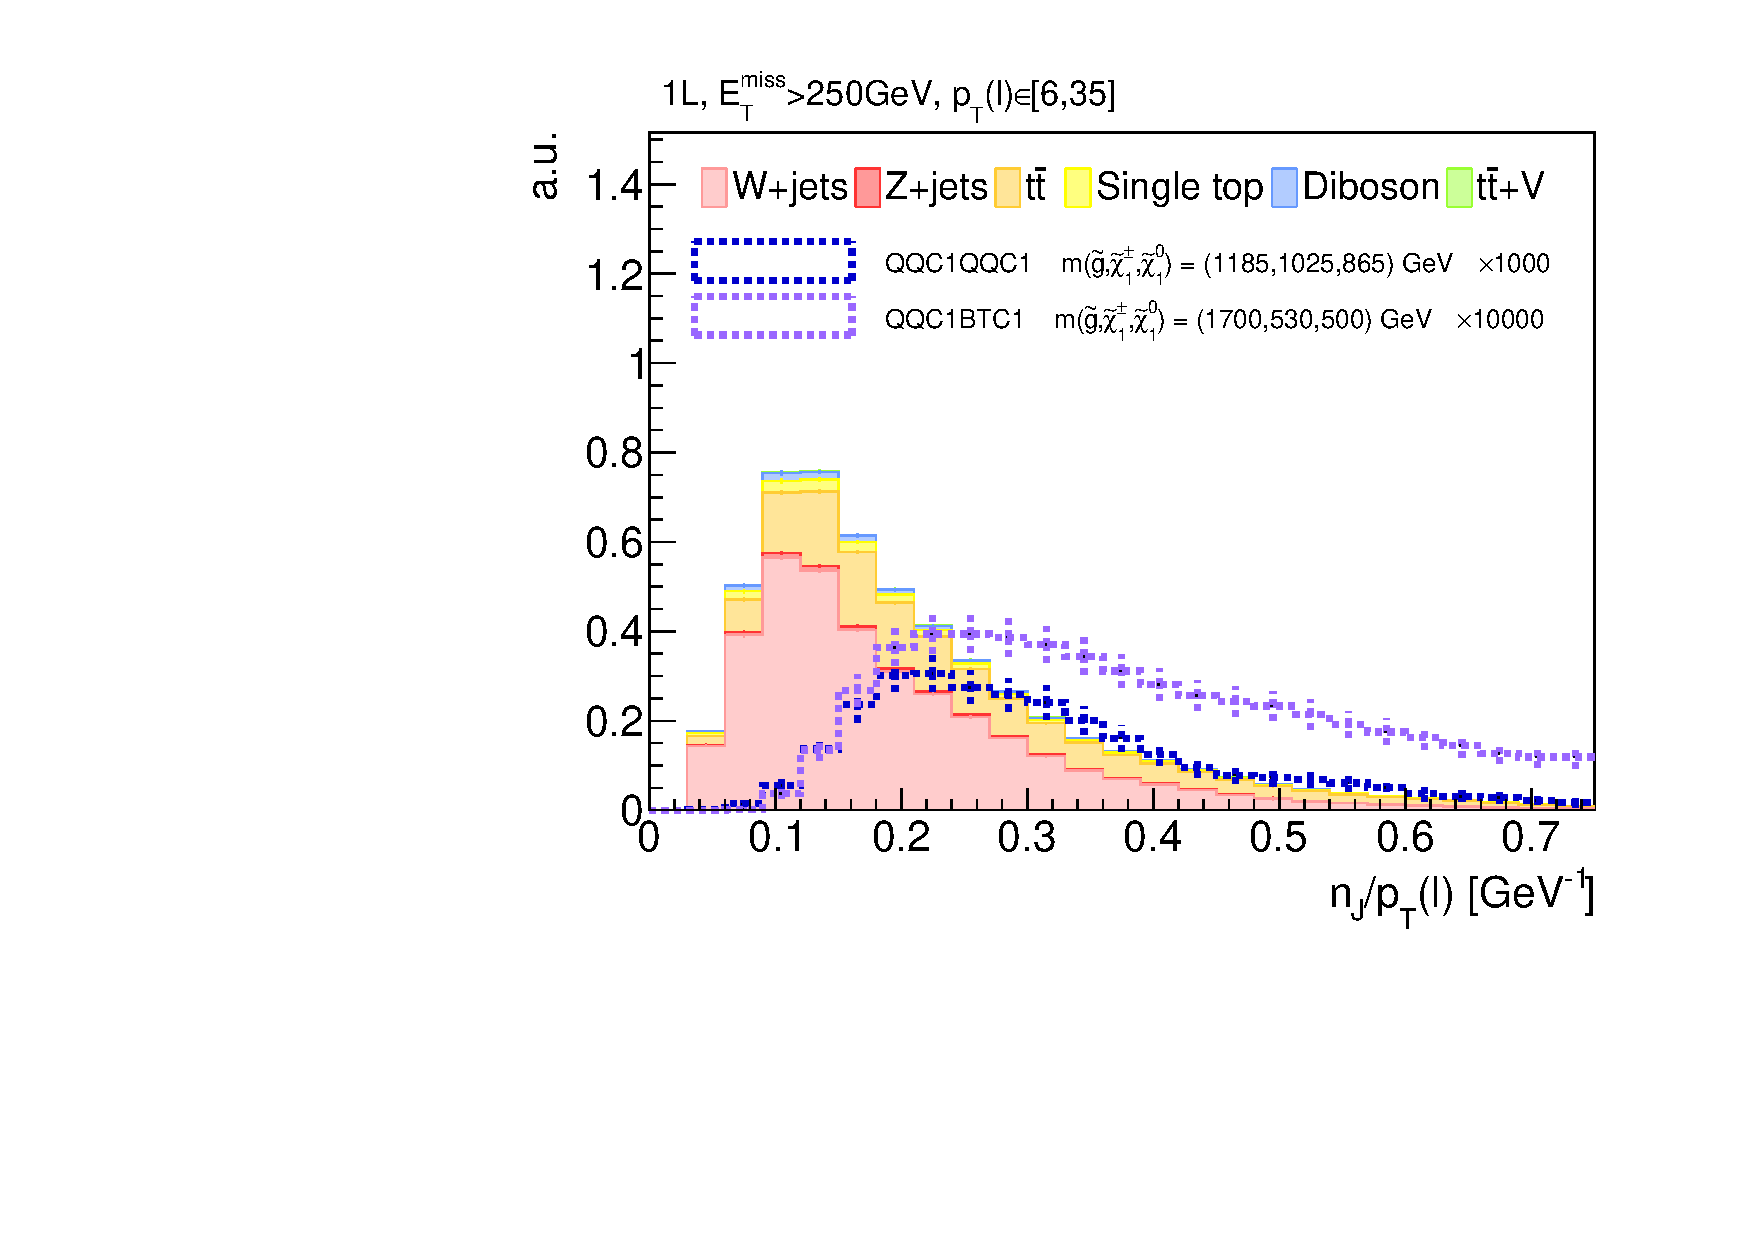
\includegraphics[width=0.48\textwidth]{figures/SRdefinition/discVar/nJetOverLepPt__Precut_softLep.pdf}}
    \subfigure[]{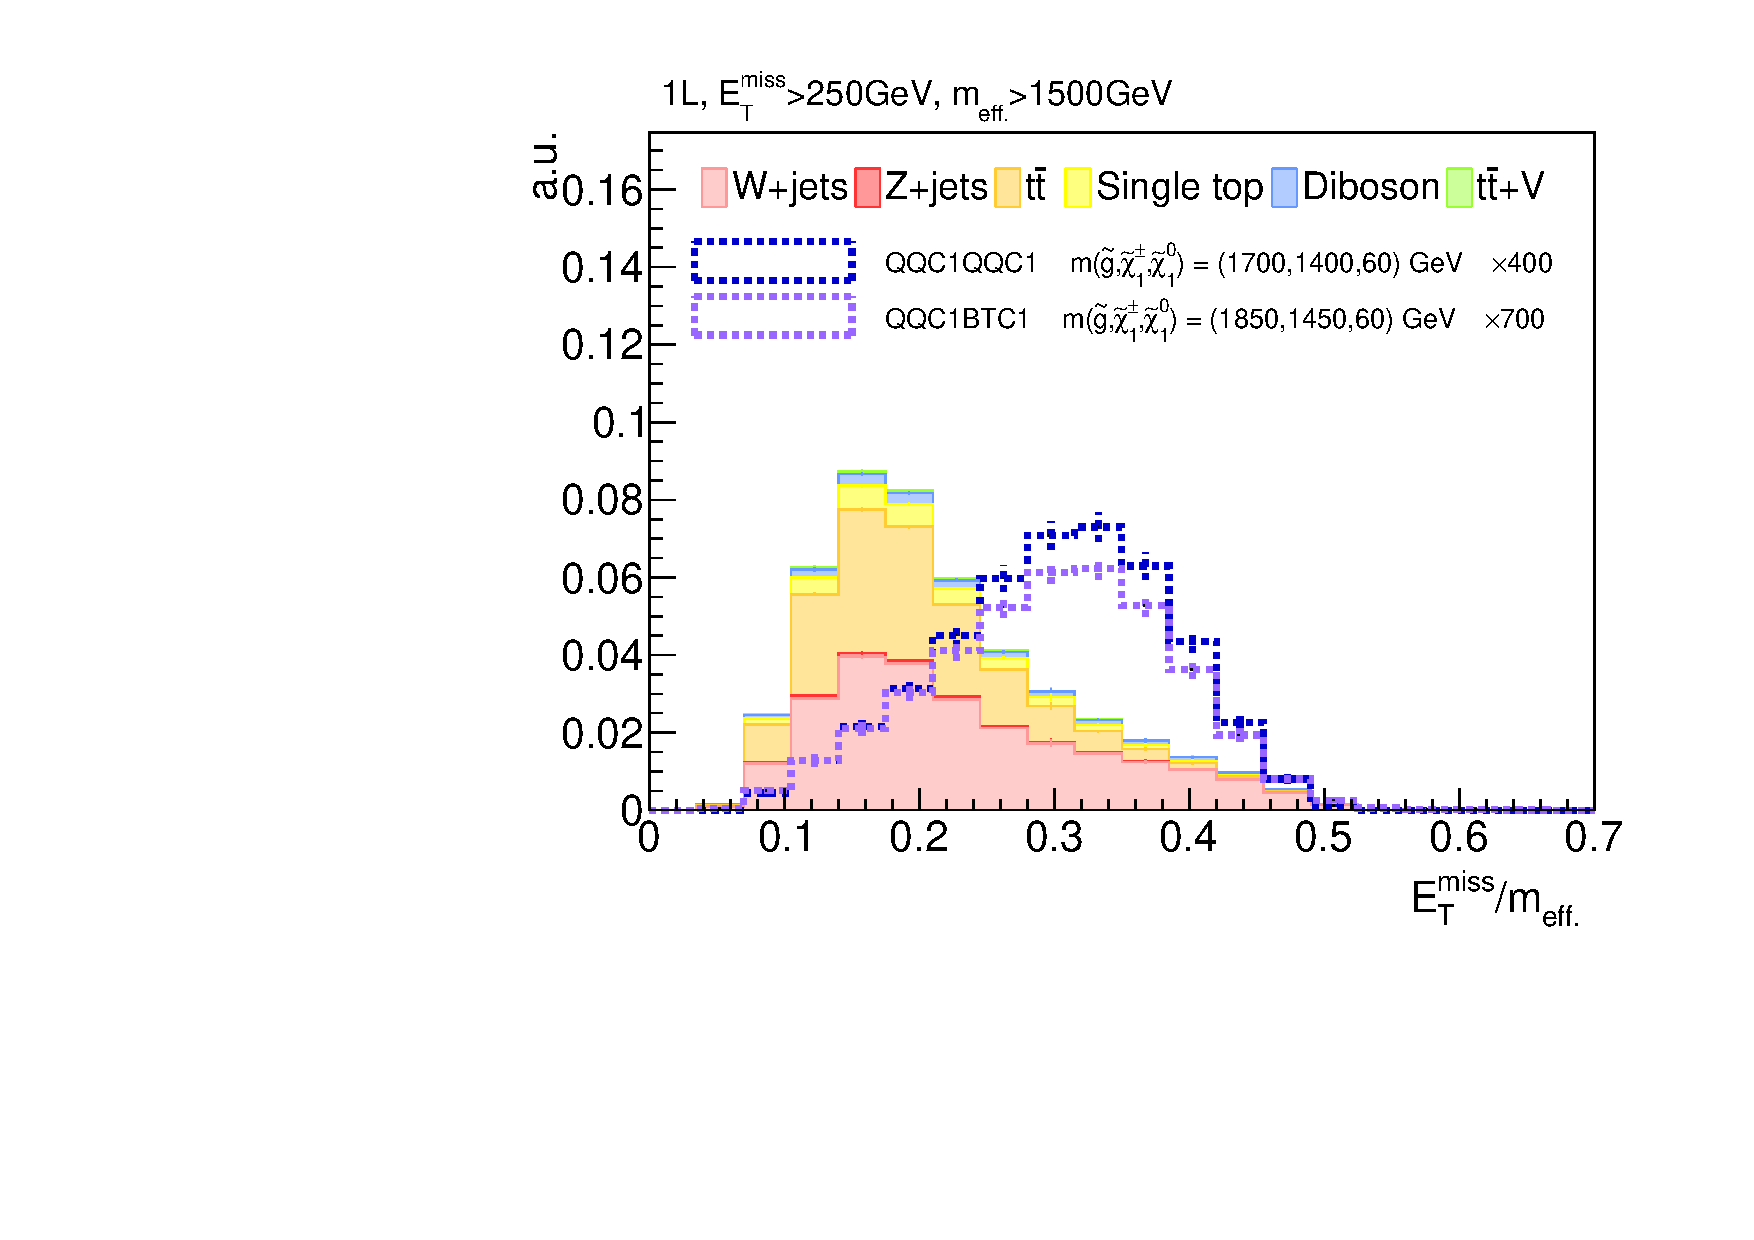
\includegraphics[width=0.48\textwidth]{figures/SRdefinition/discVar/metOverMeff__Precut_meff1500.pdf}}
    \subfigure[]{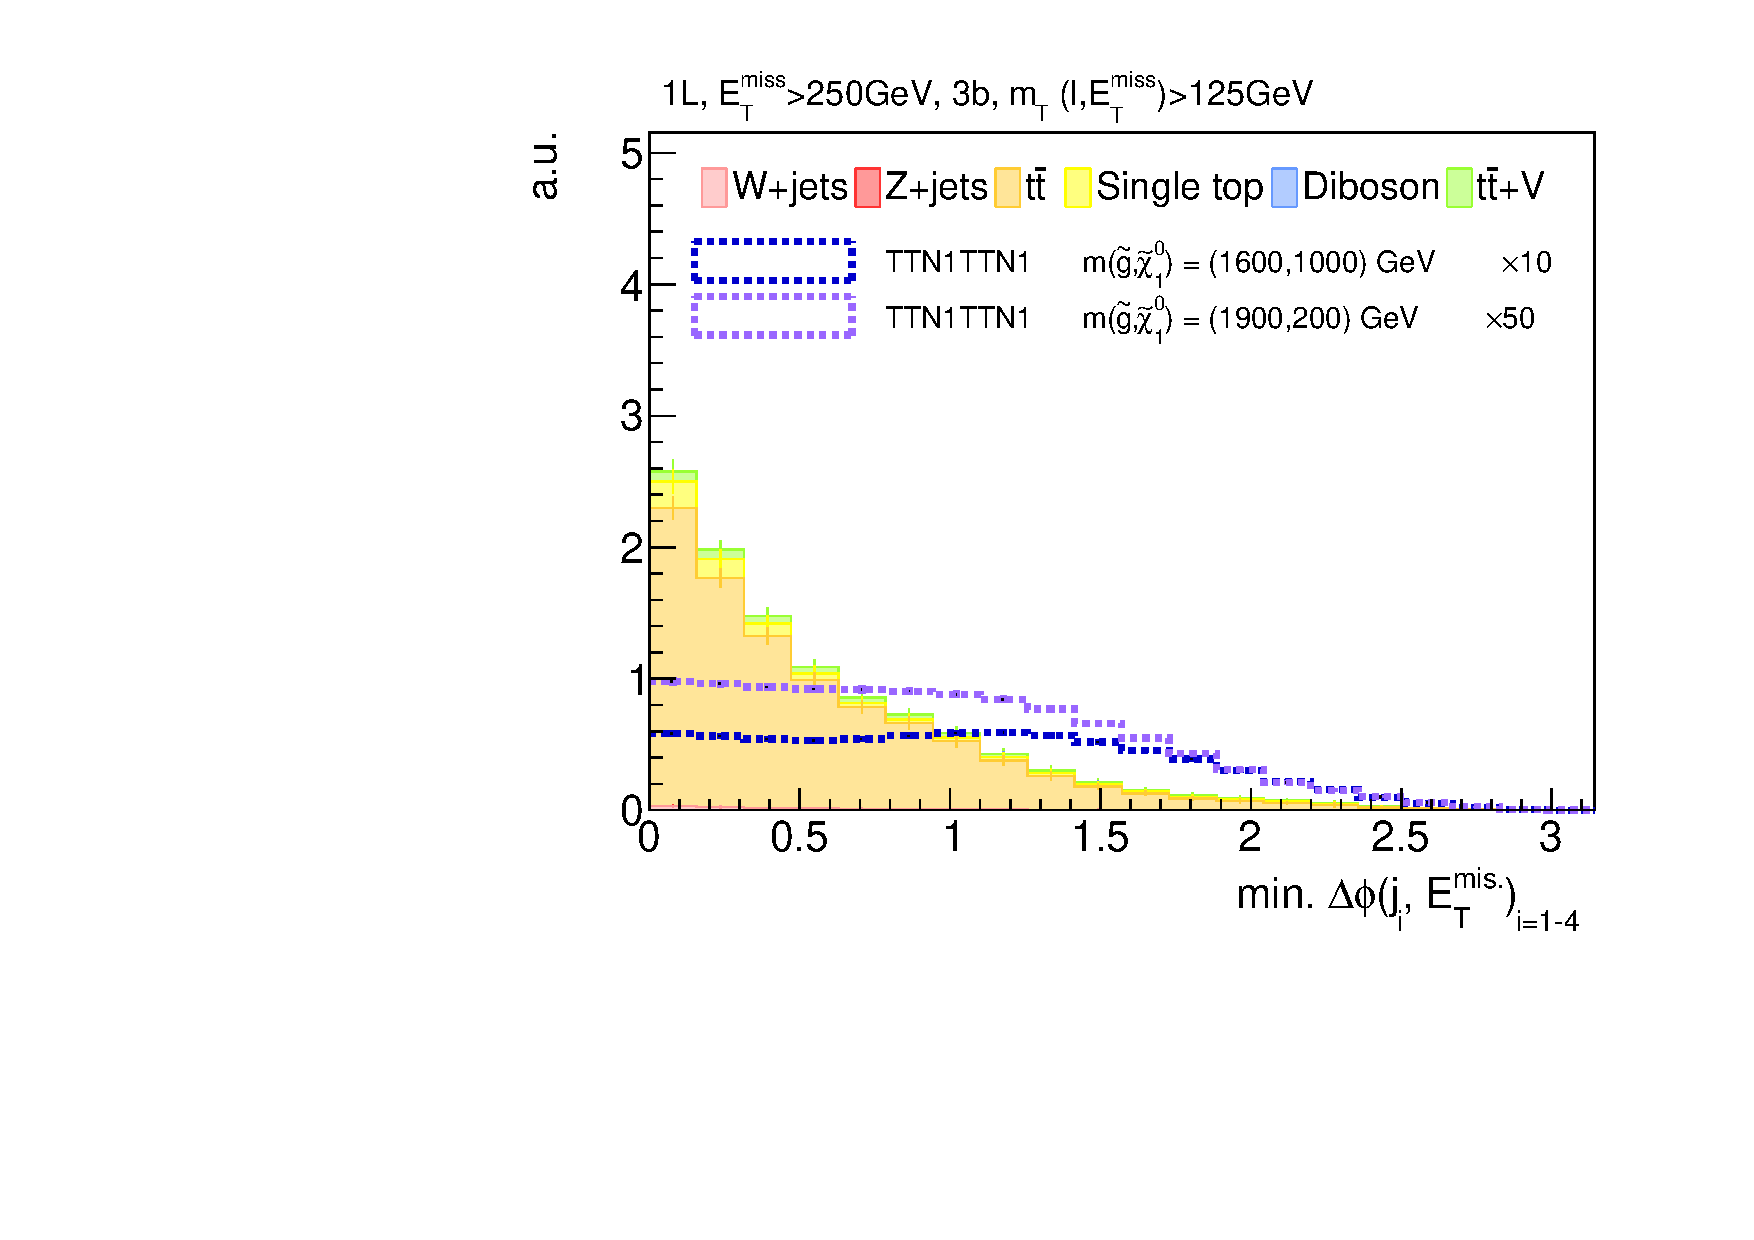
\includegraphics[width=0.48\textwidth]{figures/SRdefinition/discVar/min_dPhi_4j__Precut3B_MT125.pdf}}
    \subfigure[]{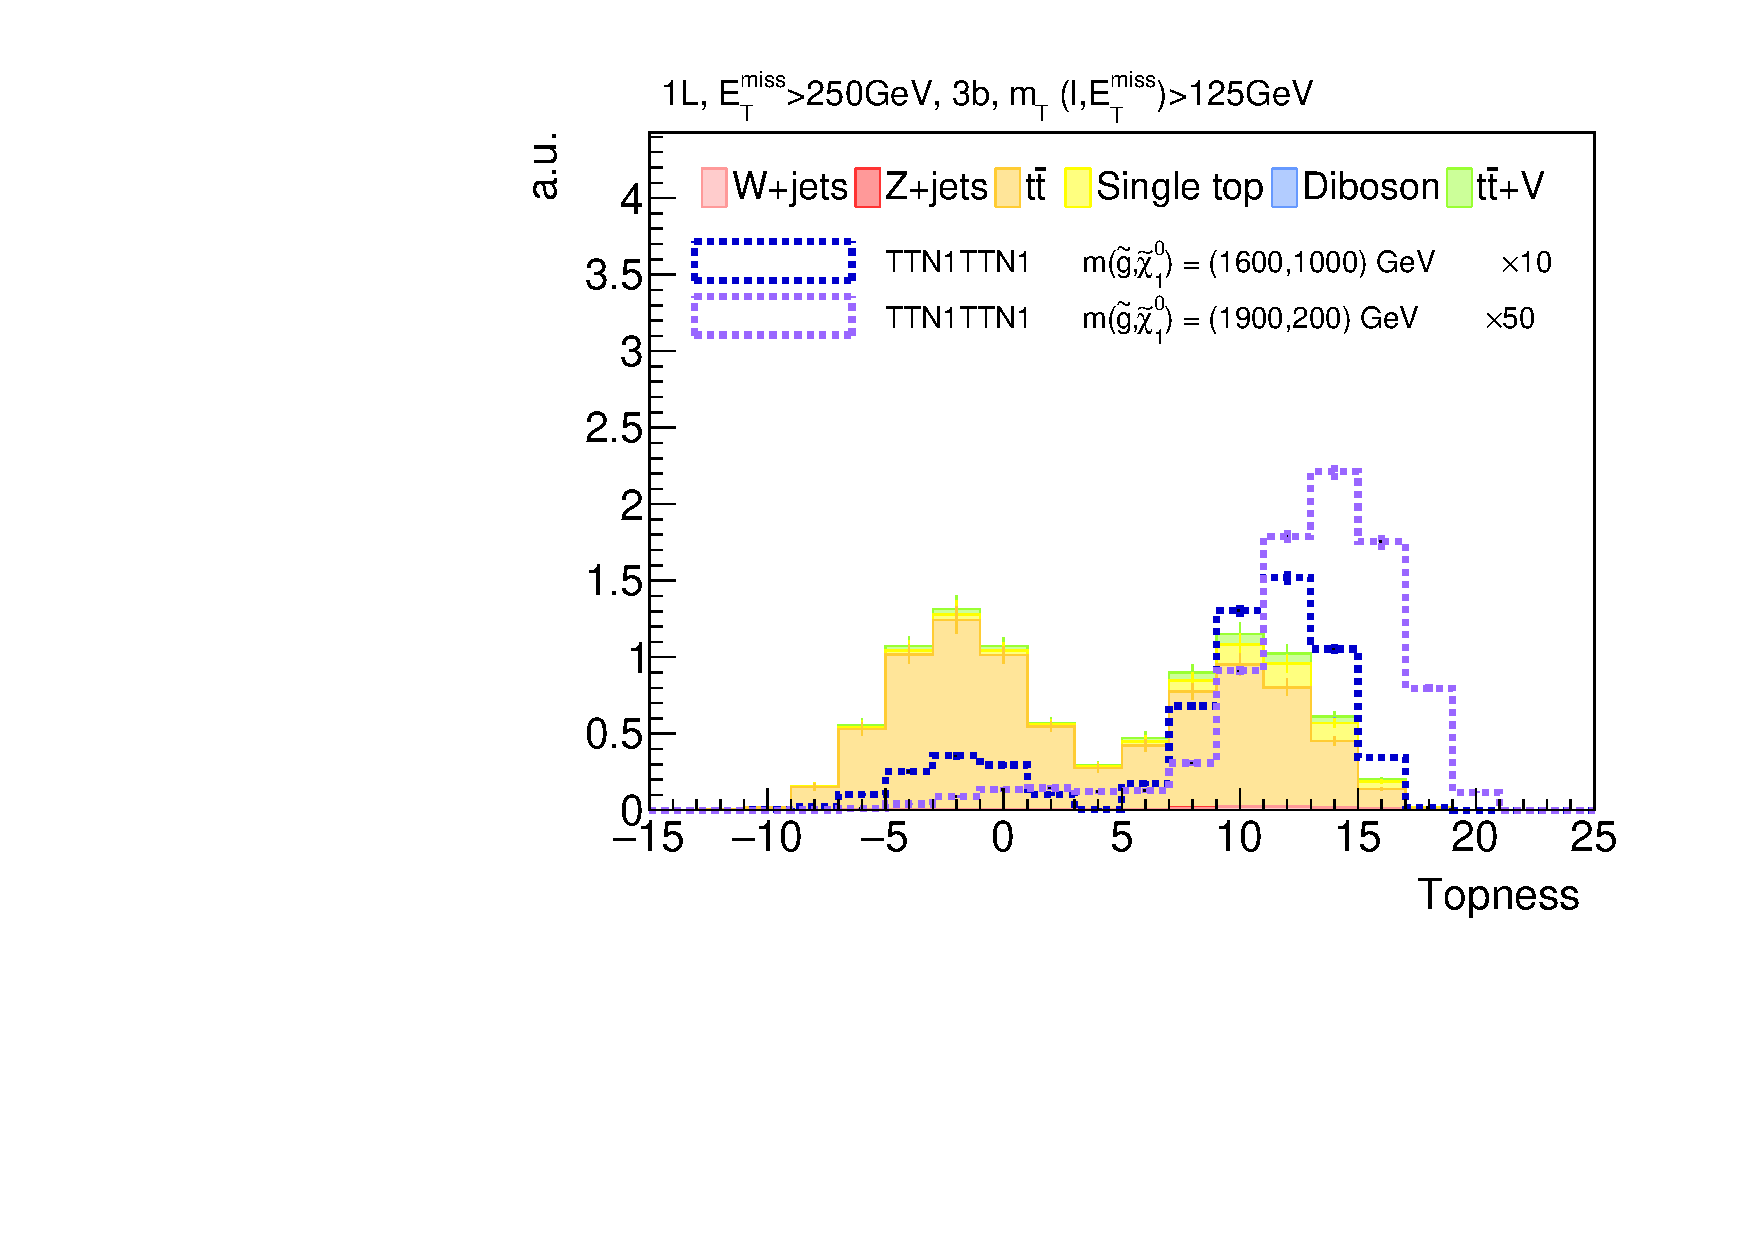
\includegraphics[width=0.48\textwidth]{figures/SRdefinition/discVar/topNess__Precut3B_MT125.pdf}}
    \caption{ 
    Distributions of discriminating variables at the preselection level.
    Soft lepton requirement: $\pt(\ell)\in[6,35]$ is applied for (b),
    and $\nBJetNoGev \geq3 \,\,\, \mt>125\gev$ is applied for (c). 
    \label{fig::SRdefinition::distVar2}
    }
\end{figure}


The trend of the kinematical variables over the mass grids are shown in Fig. \ref{fig::SRdefinition::kineMap_QQC1QQC1_x12}-\ref{fig::SRdefinition::kineMap_TTN1TTN1}. The color scale (z-axis) indicates the mean of the distribution in the variables, for the signal process in the mass point designated by the xy-coordinate. Three QQC1QQC1 grids (``x=1/2'', $''\mLSP=60\gev''$ and $''\dmc=30\gev''$) and one TTN1TTN1 grid are displayed as the benchmark model for BV/BT signal regions and the 3B signal regions respectively. 

One can find that the variables related to transverse momenta of outgoing particles such as $\meffInc$, $\lepPt$ and $\met$ simply scale with the mass splitting, while the other variables such as aplanarity and $\metOverMeff$ etc. are sensitive to the relative mass spilitting, therefore helpful in defining SR \textbf{Low-x}/\textbf{High-x}.
\clearpage
    
\begin{figure}[h]
  \centering
%    \subfigure[]{\includegraphics[width=0.45\textwidth]{figures/SRdefinition/kineMap/GG_symQQC1_x12_nJet30.pdf}}
    \subfigure[]{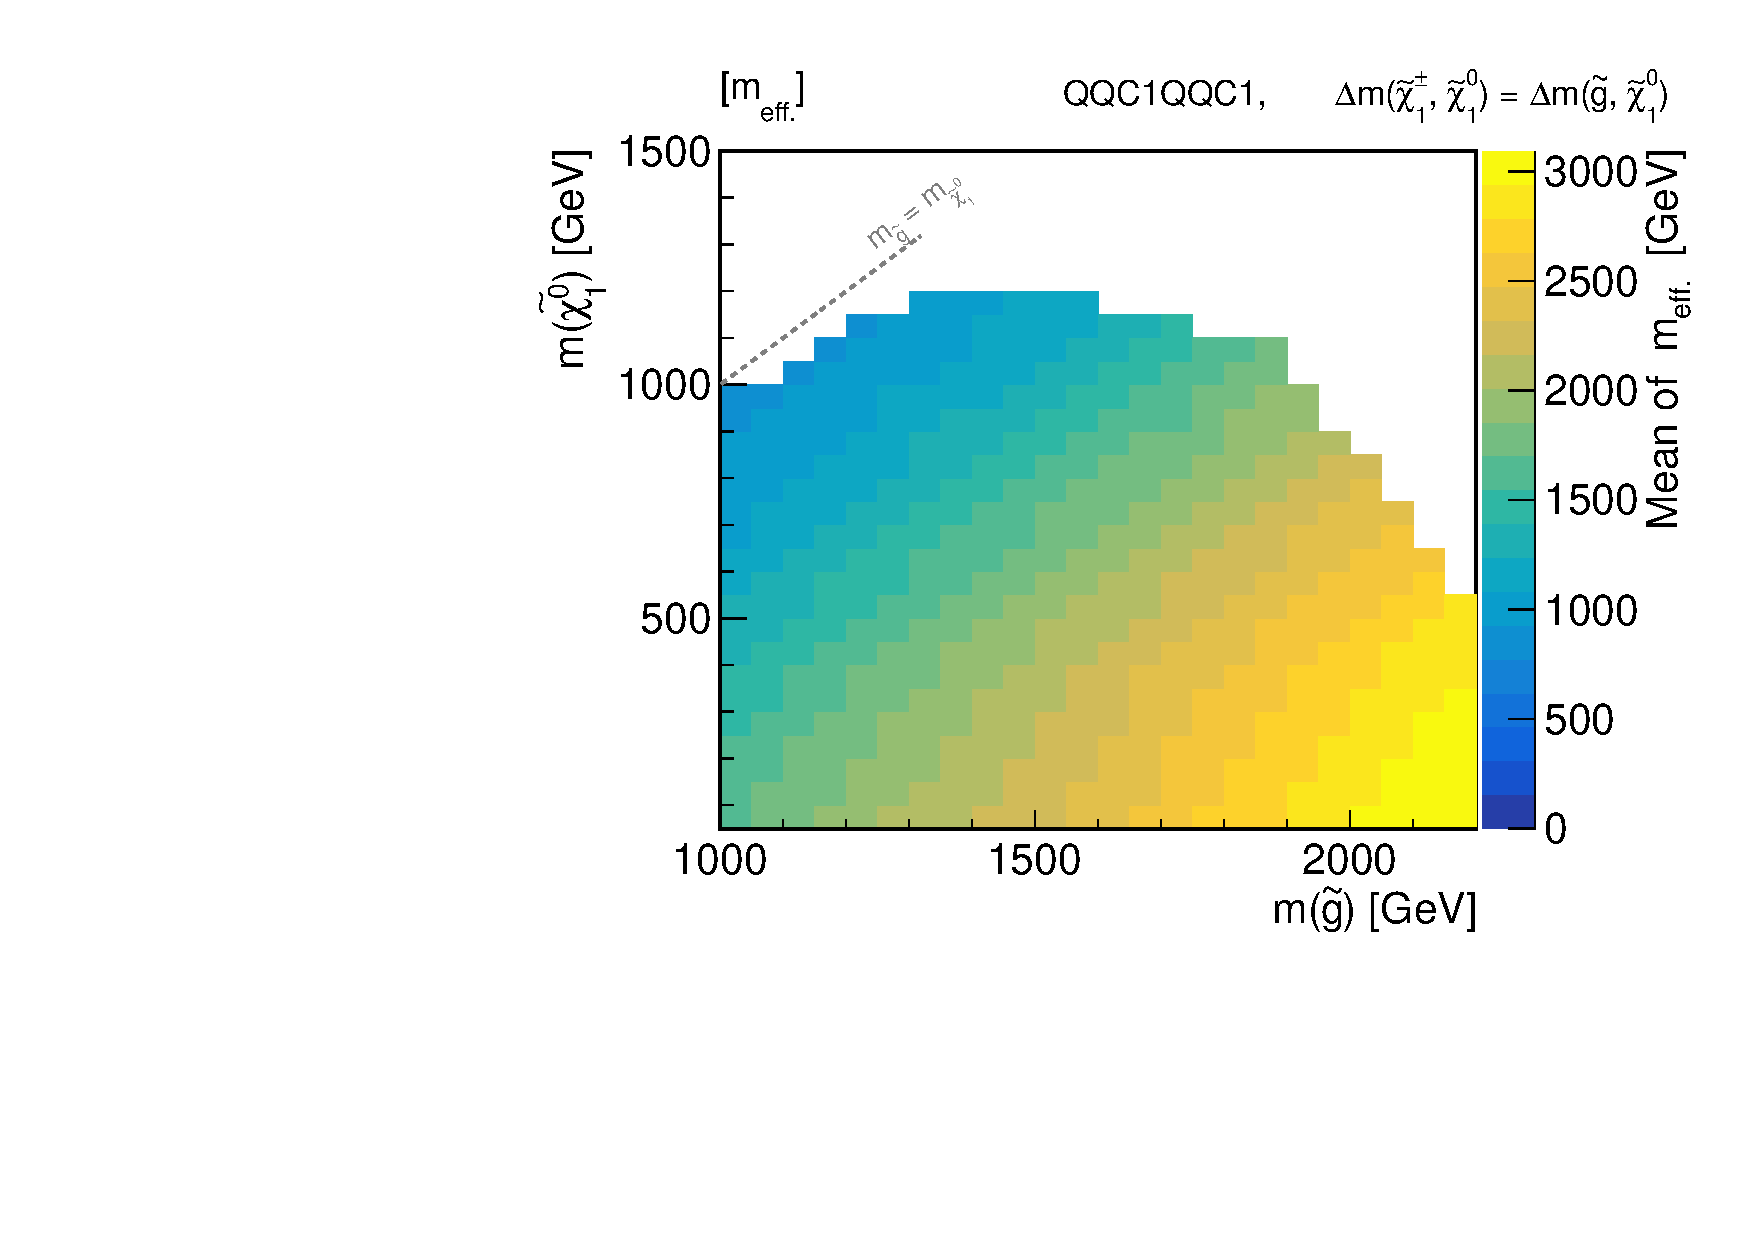
\includegraphics[width=0.45\textwidth]{figures/SRdefinition/kineMap/GG_symQQC1_x12_meff.pdf}}
    \subfigure[]{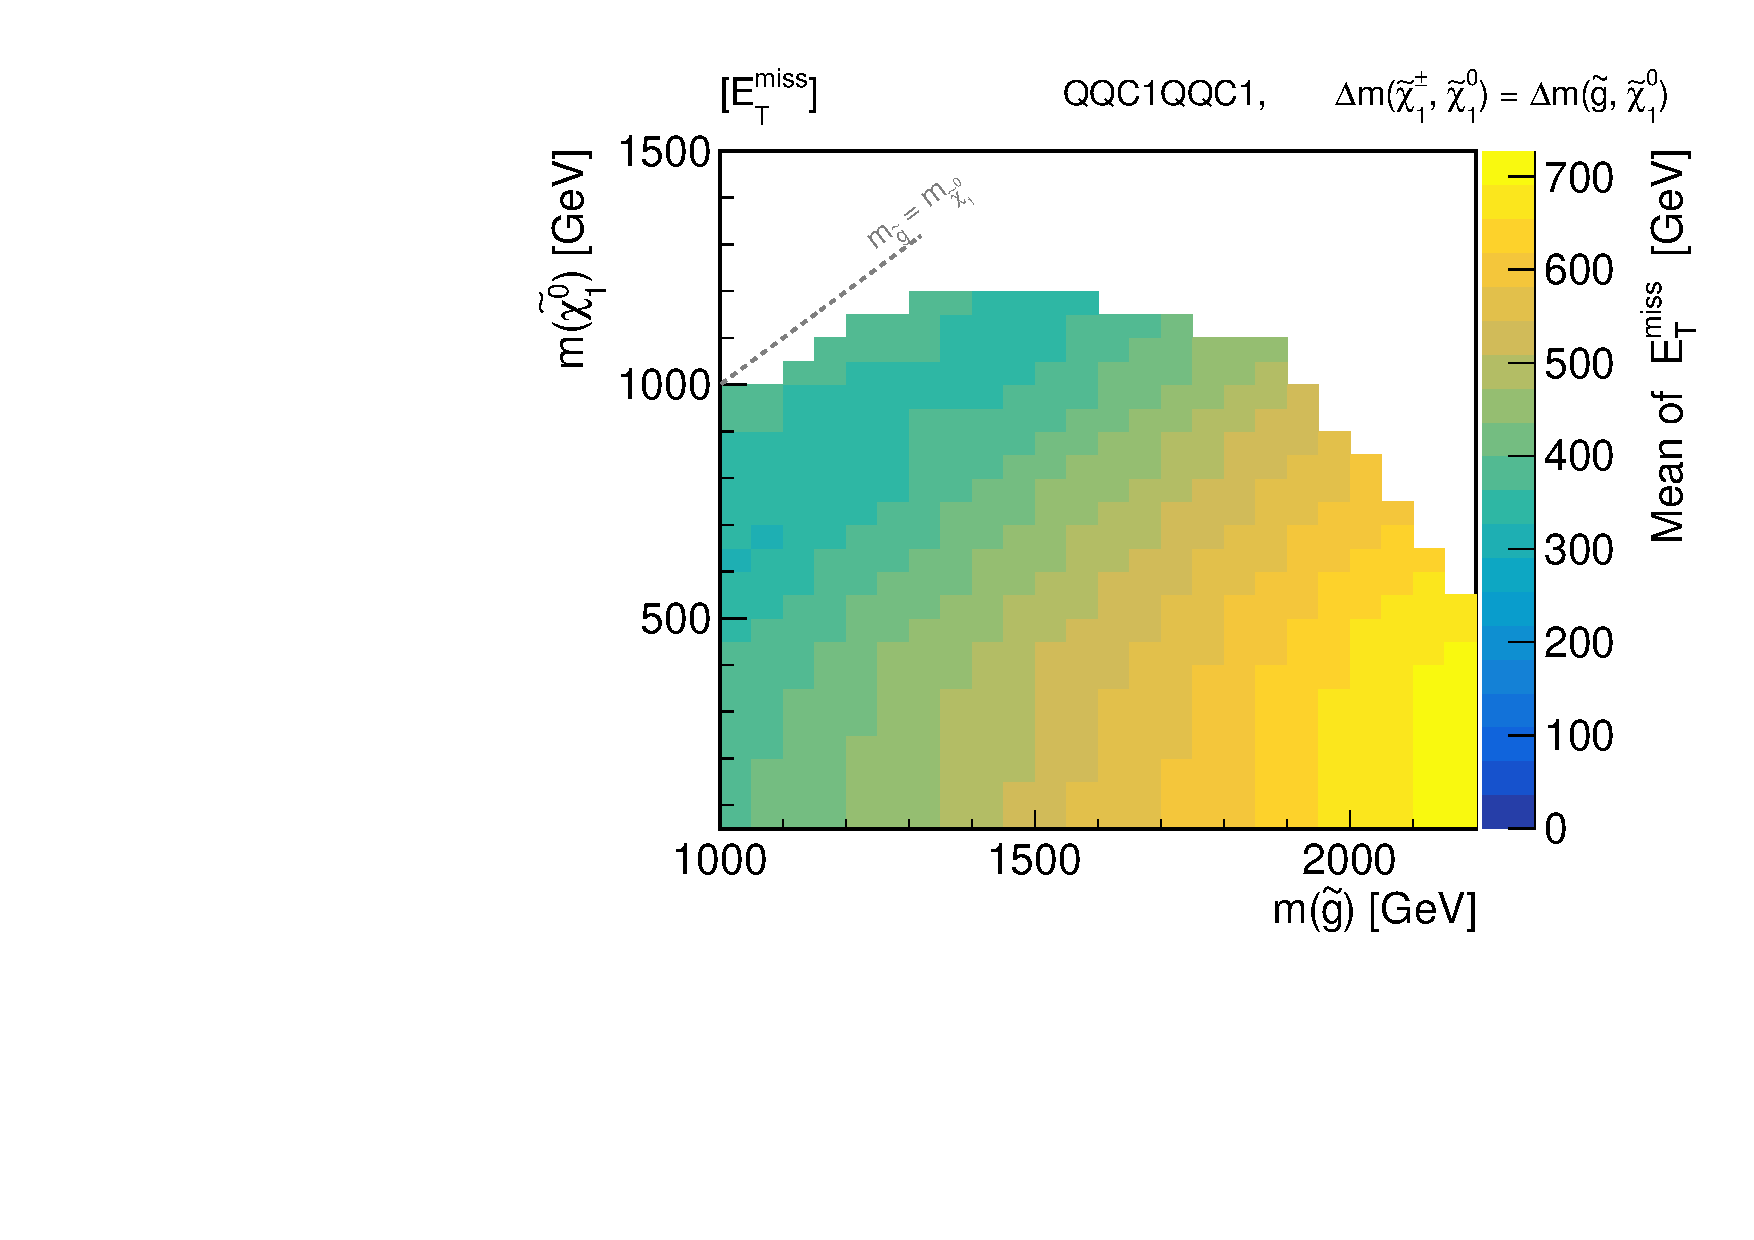
\includegraphics[width=0.45\textwidth]{figures/SRdefinition/kineMap/GG_symQQC1_x12_met.pdf}}
    \subfigure[]{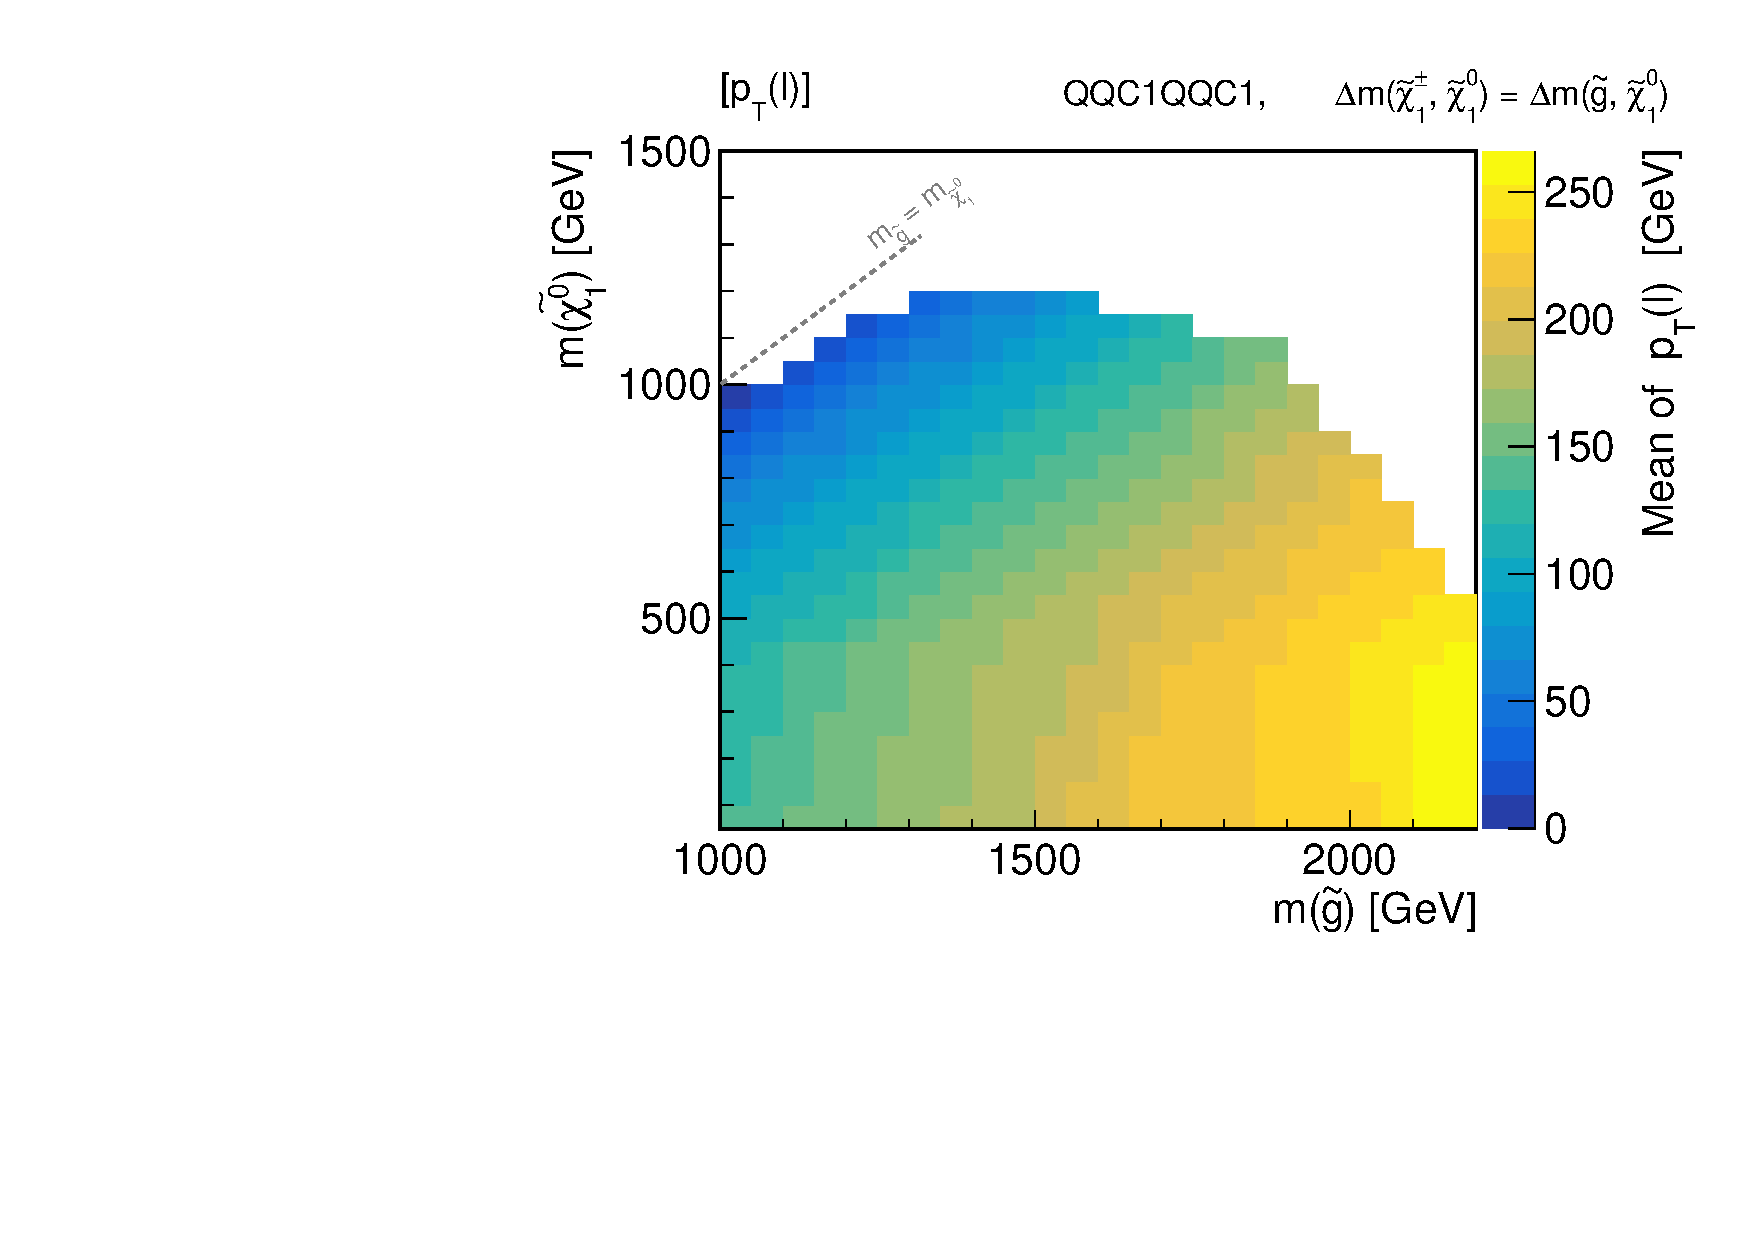
\includegraphics[width=0.45\textwidth]{figures/SRdefinition/kineMap/GG_symQQC1_x12_lep1Pt.pdf}}
    \subfigure[]{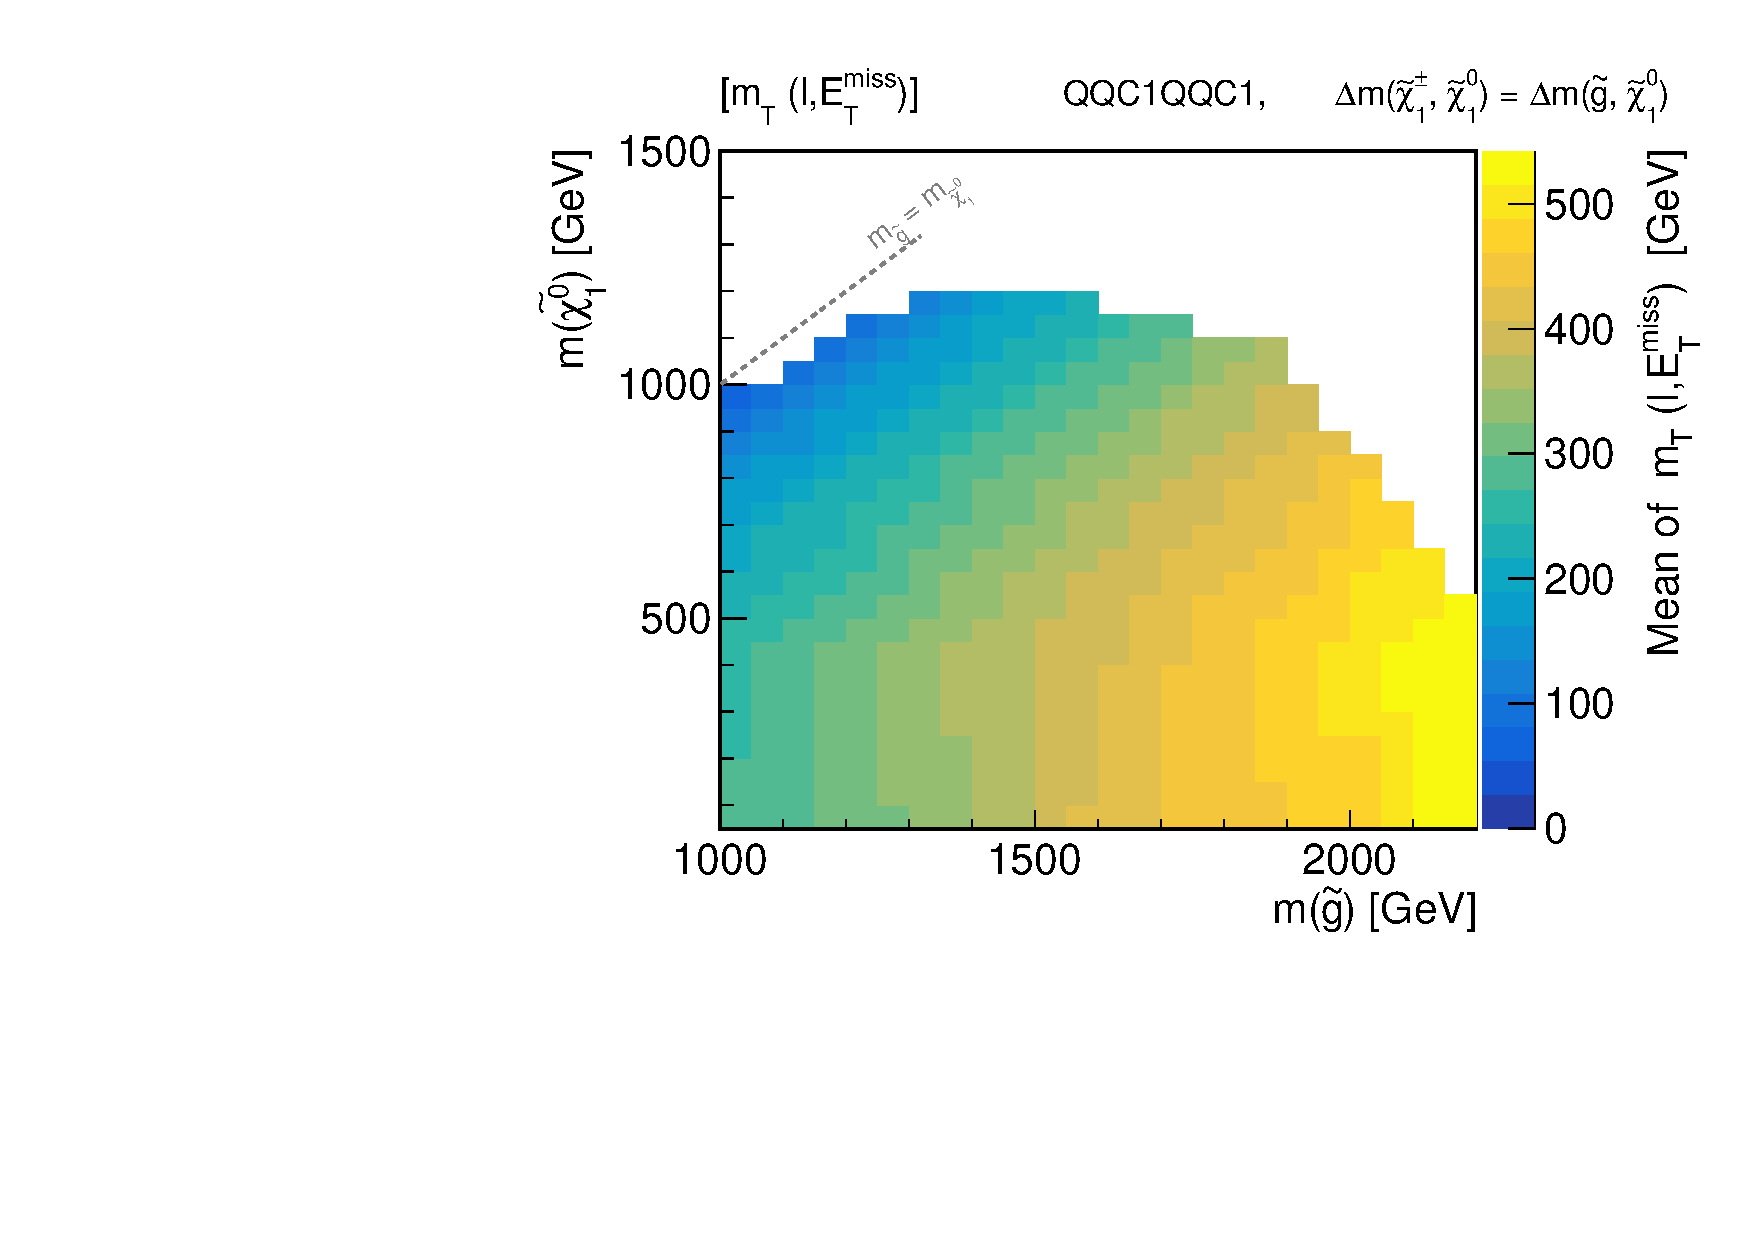
\includegraphics[width=0.45\textwidth]{figures/SRdefinition/kineMap/GG_symQQC1_x12_mt.pdf}}
    \subfigure[]{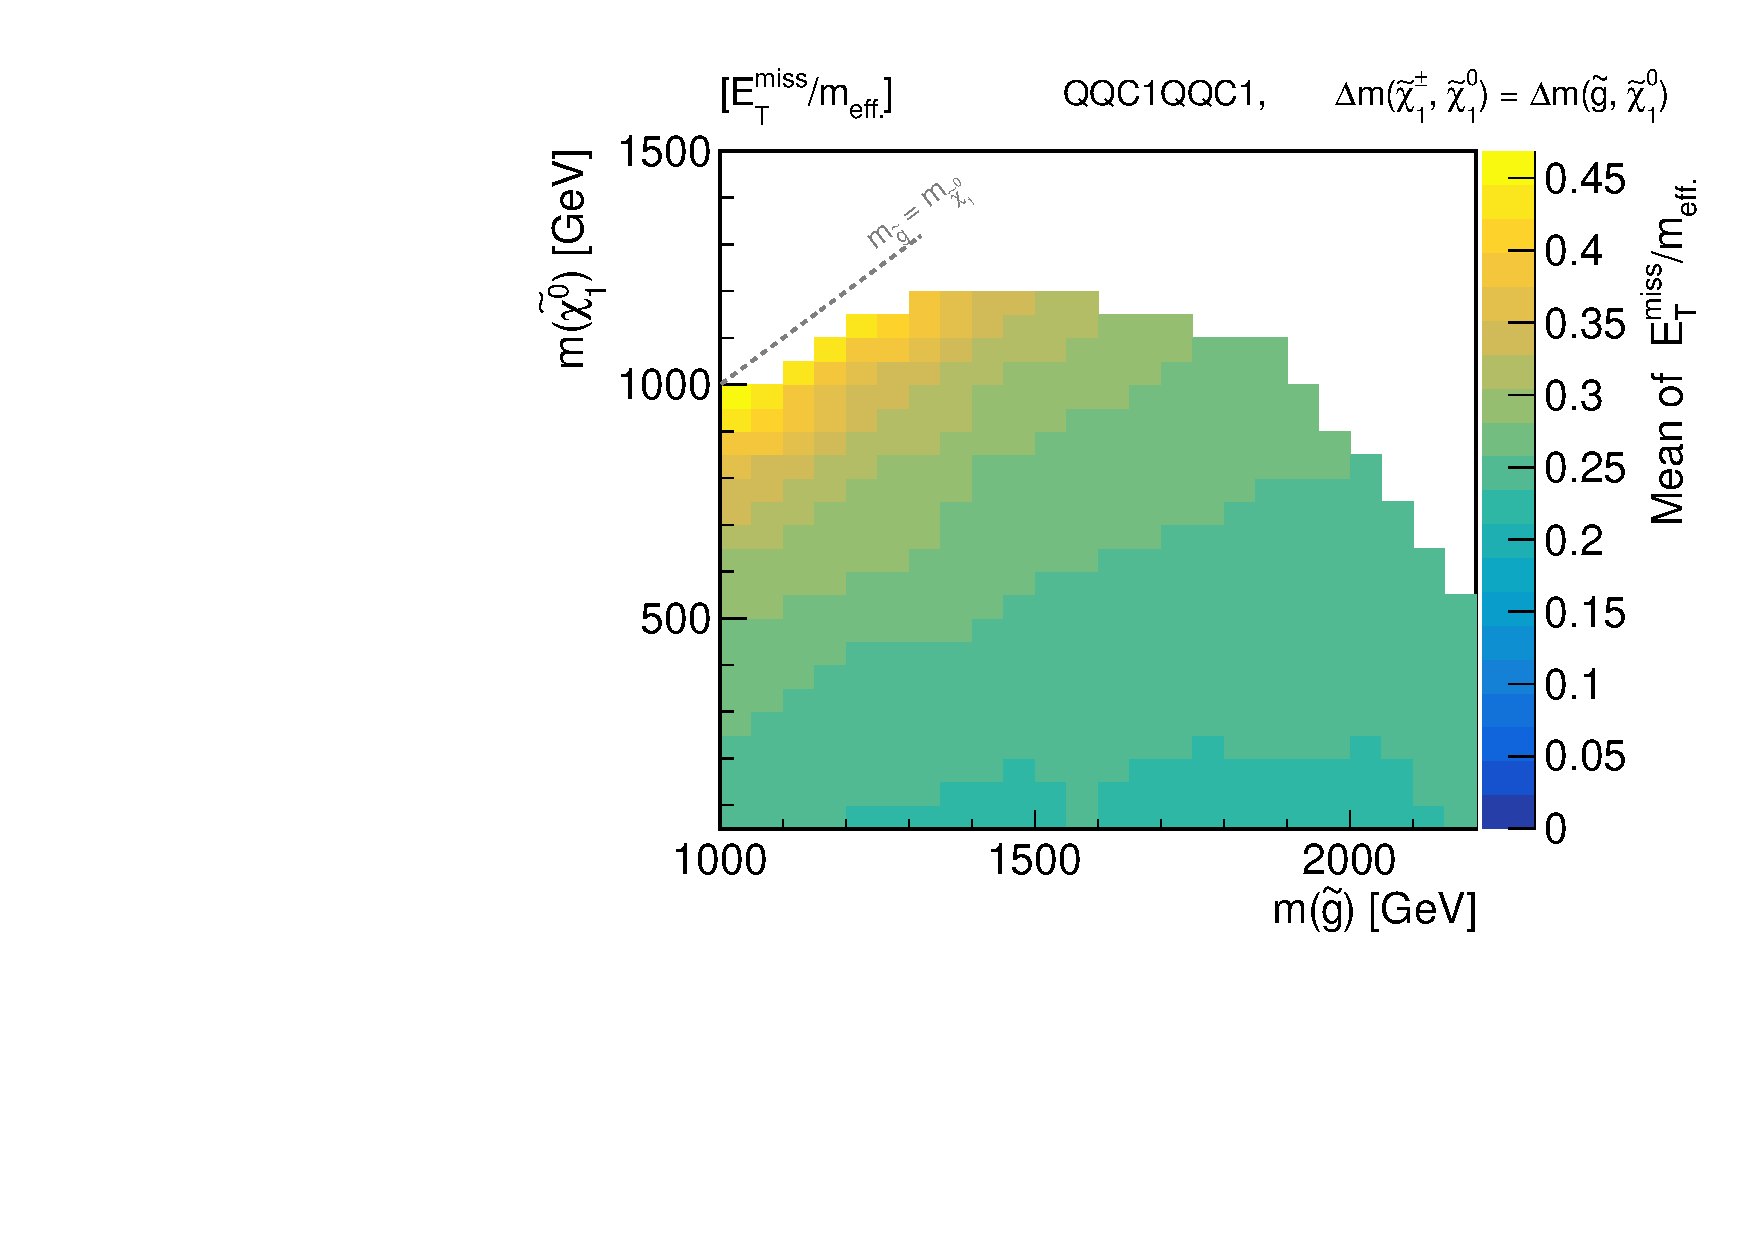
\includegraphics[width=0.45\textwidth]{figures/SRdefinition/kineMap/GG_symQQC1_x12_metOverMeff.pdf}}
    \subfigure[]{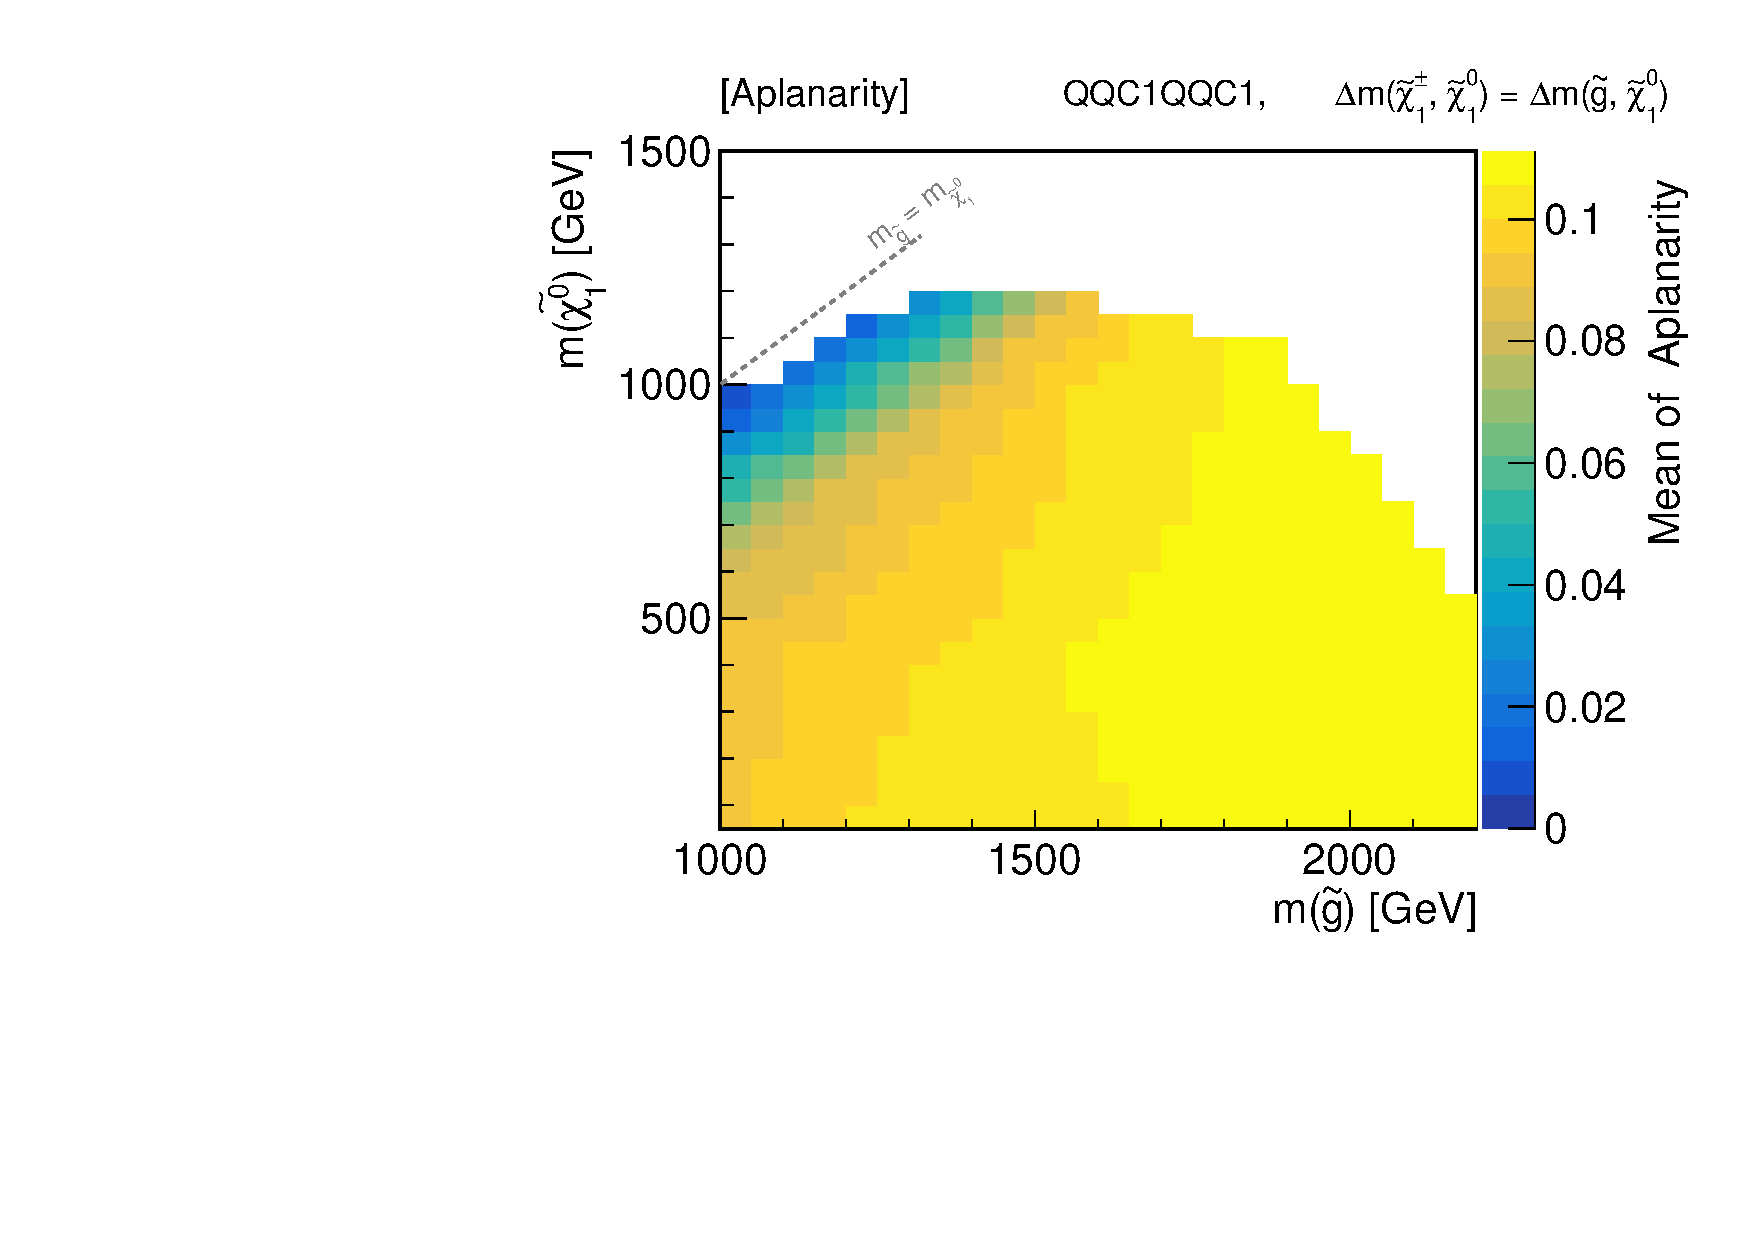
\includegraphics[width=0.45\textwidth]{figures/SRdefinition/kineMap/GG_symQQC1_x12_LepAplanarity.pdf}}
    \caption{ Mean of (a) $\meffInc$ (b) $\met$ (c) $\lepPt$ (d) $\mt$ (e) $\metOverMeff$ (f) aplanarity, for the QQC1QQC1 \xhalf grid, after the pre-selection. 
      \label{fig::SRdefinition::kineMap_QQC1QQC1_x12} 
    }
\end{figure}
 

\begin{figure}[h]
  \centering
%    \subfigure[]{\includegraphics[width=0.45\textwidth]{figures/SRdefinition/kineMap/GG_symQQC1_varx_nJet30.pdf}}
    \subfigure[]{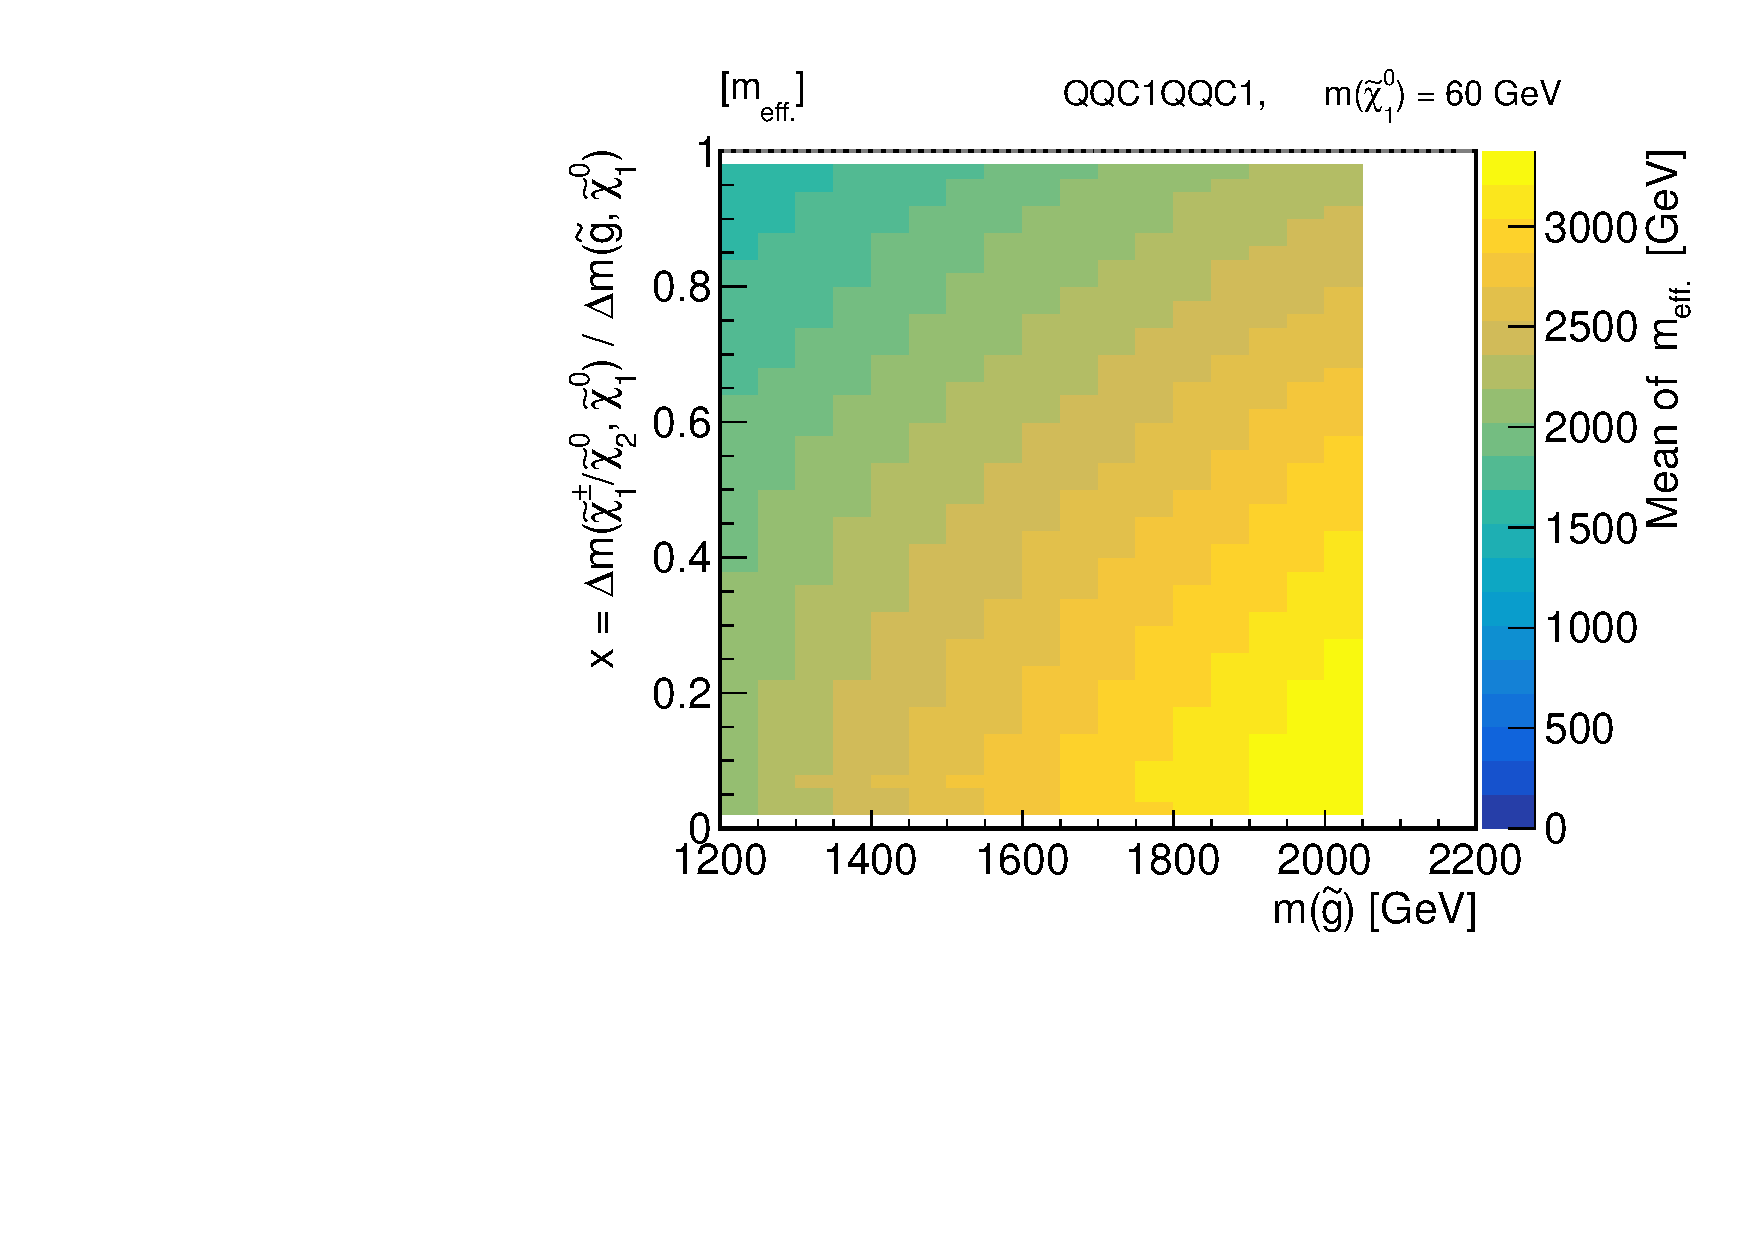
\includegraphics[width=0.45\textwidth]{figures/SRdefinition/kineMap/GG_symQQC1_varx_meff.pdf}}
    \subfigure[]{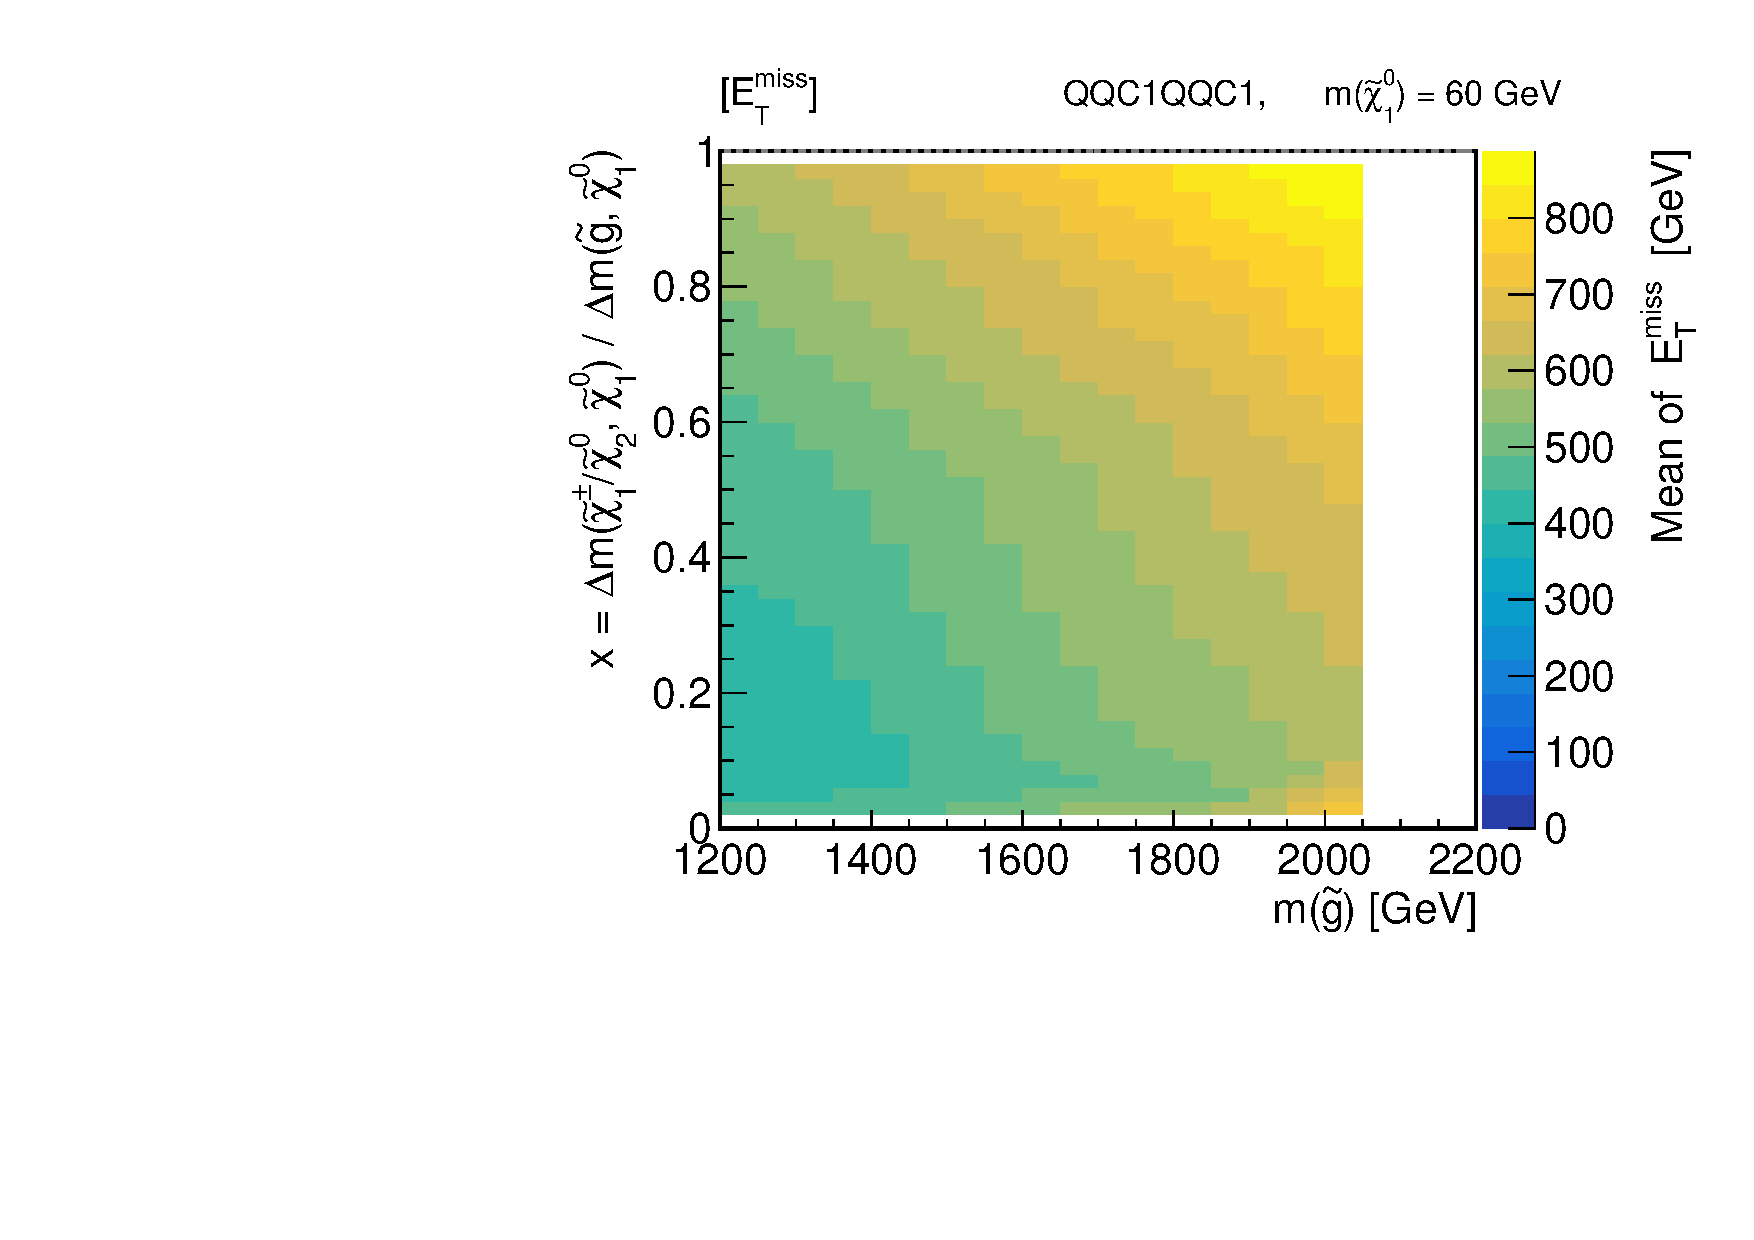
\includegraphics[width=0.45\textwidth]{figures/SRdefinition/kineMap/GG_symQQC1_varx_met.pdf}}
    \subfigure[]{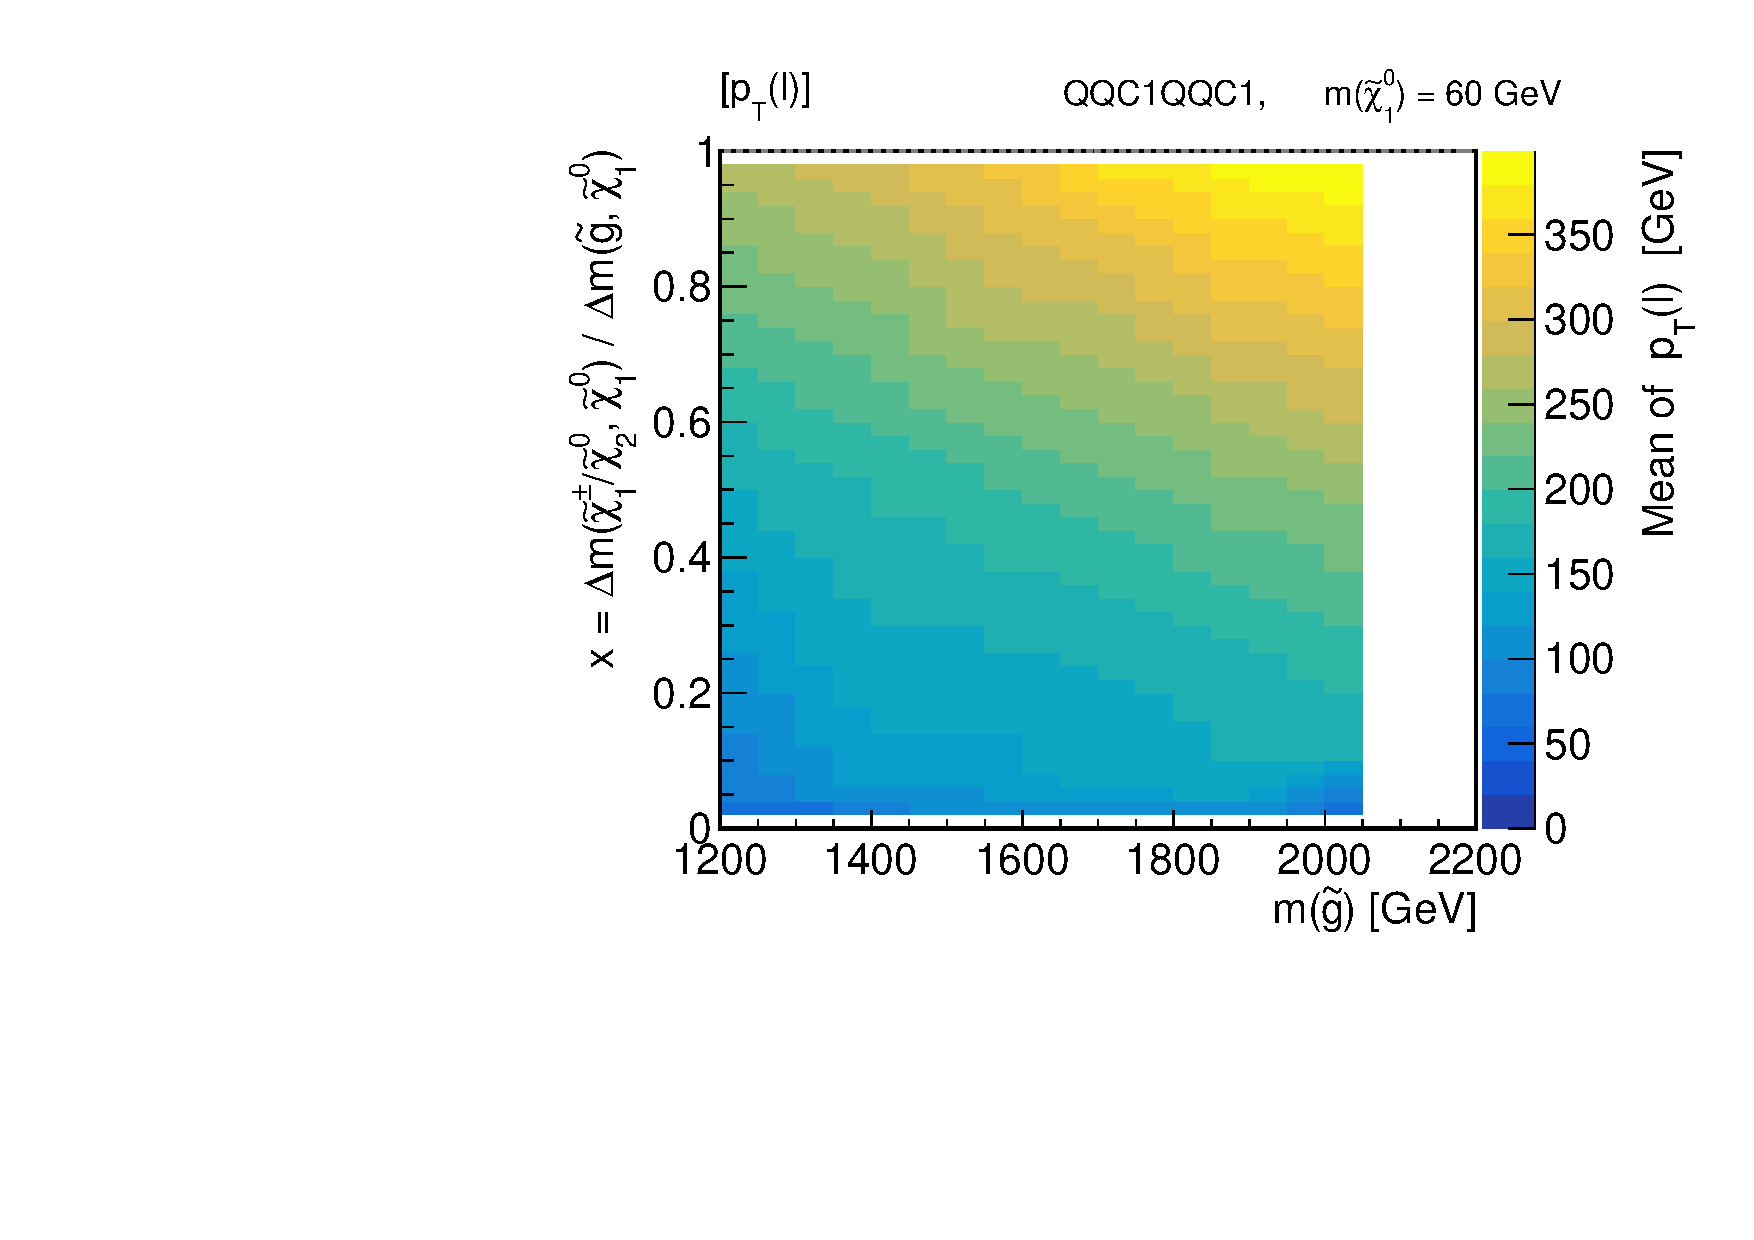
\includegraphics[width=0.45\textwidth]{figures/SRdefinition/kineMap/GG_symQQC1_varx_lep1Pt.pdf}}
    \subfigure[]{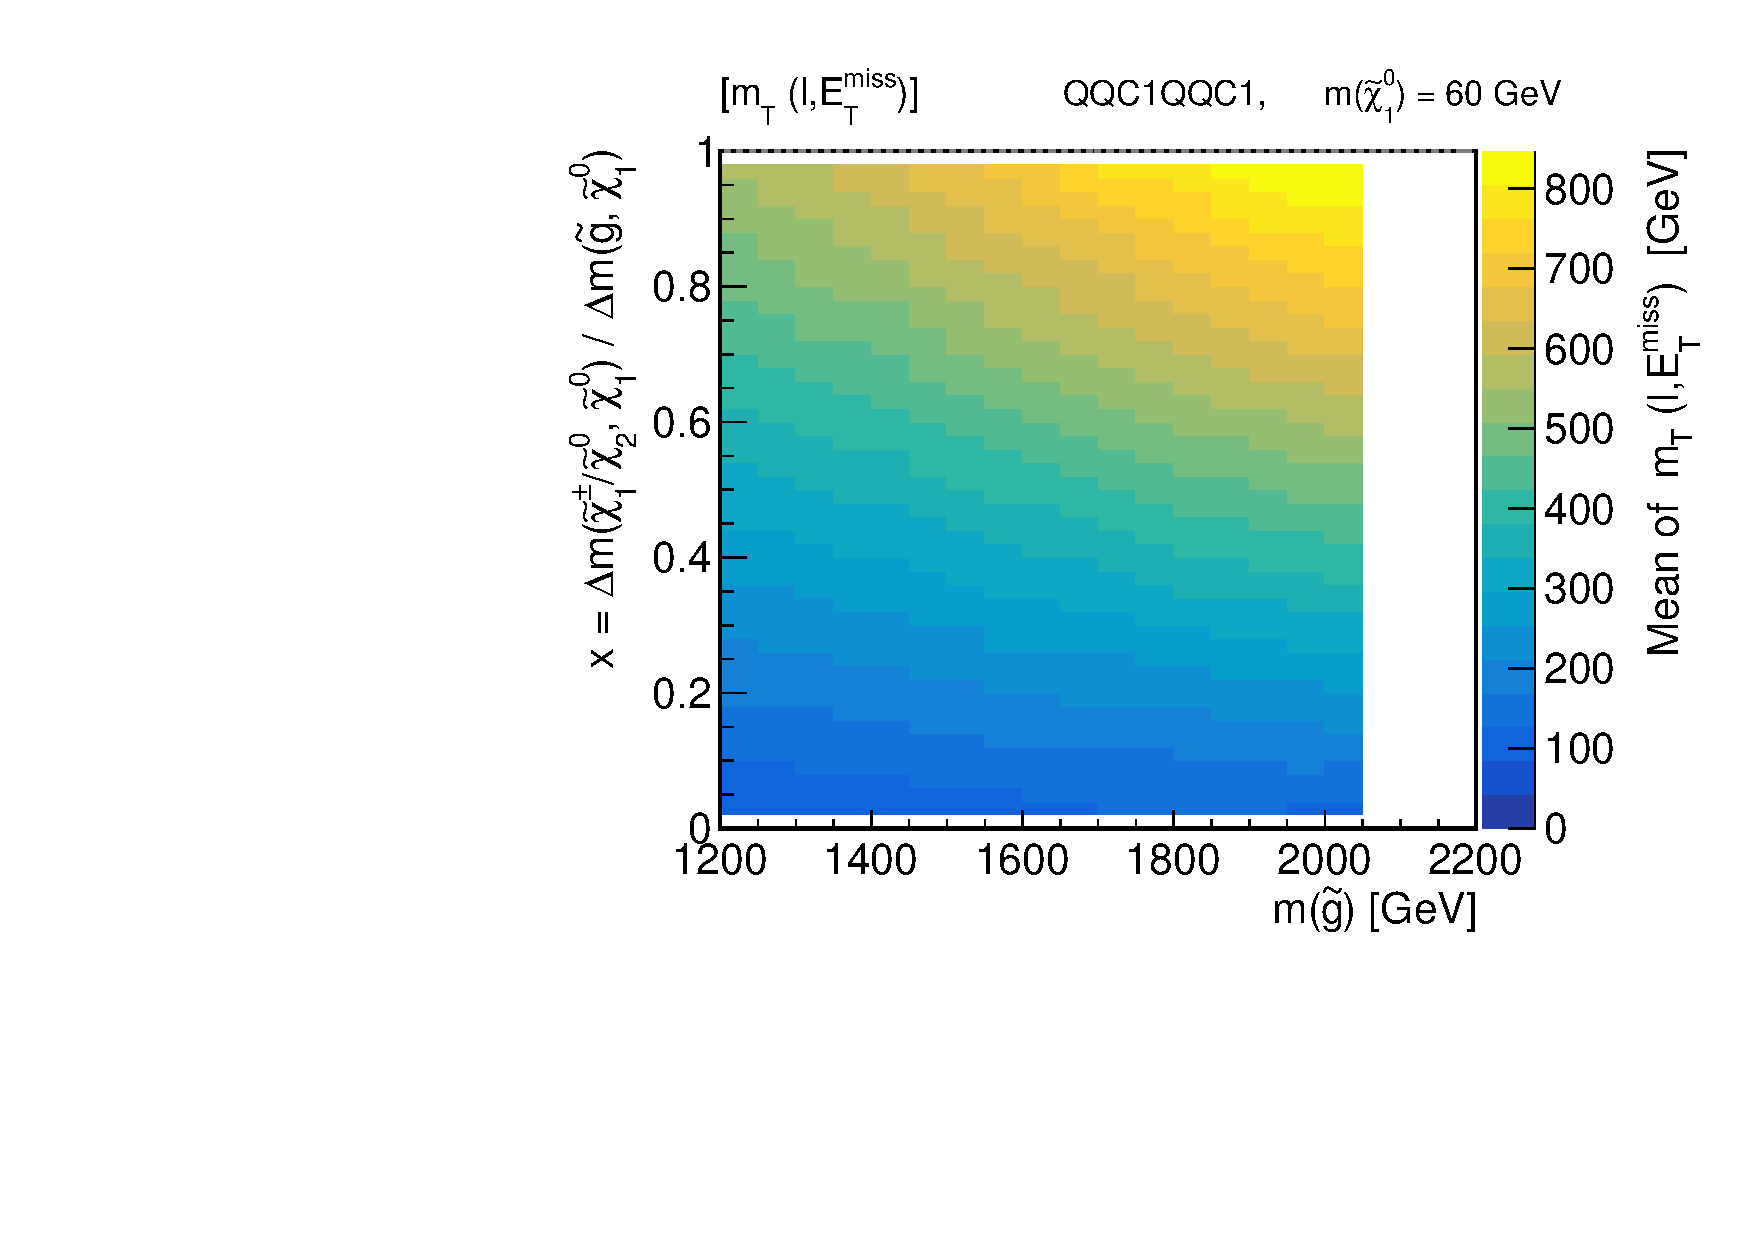
\includegraphics[width=0.45\textwidth]{figures/SRdefinition/kineMap/GG_symQQC1_varx_mt.pdf}}
    \subfigure[]{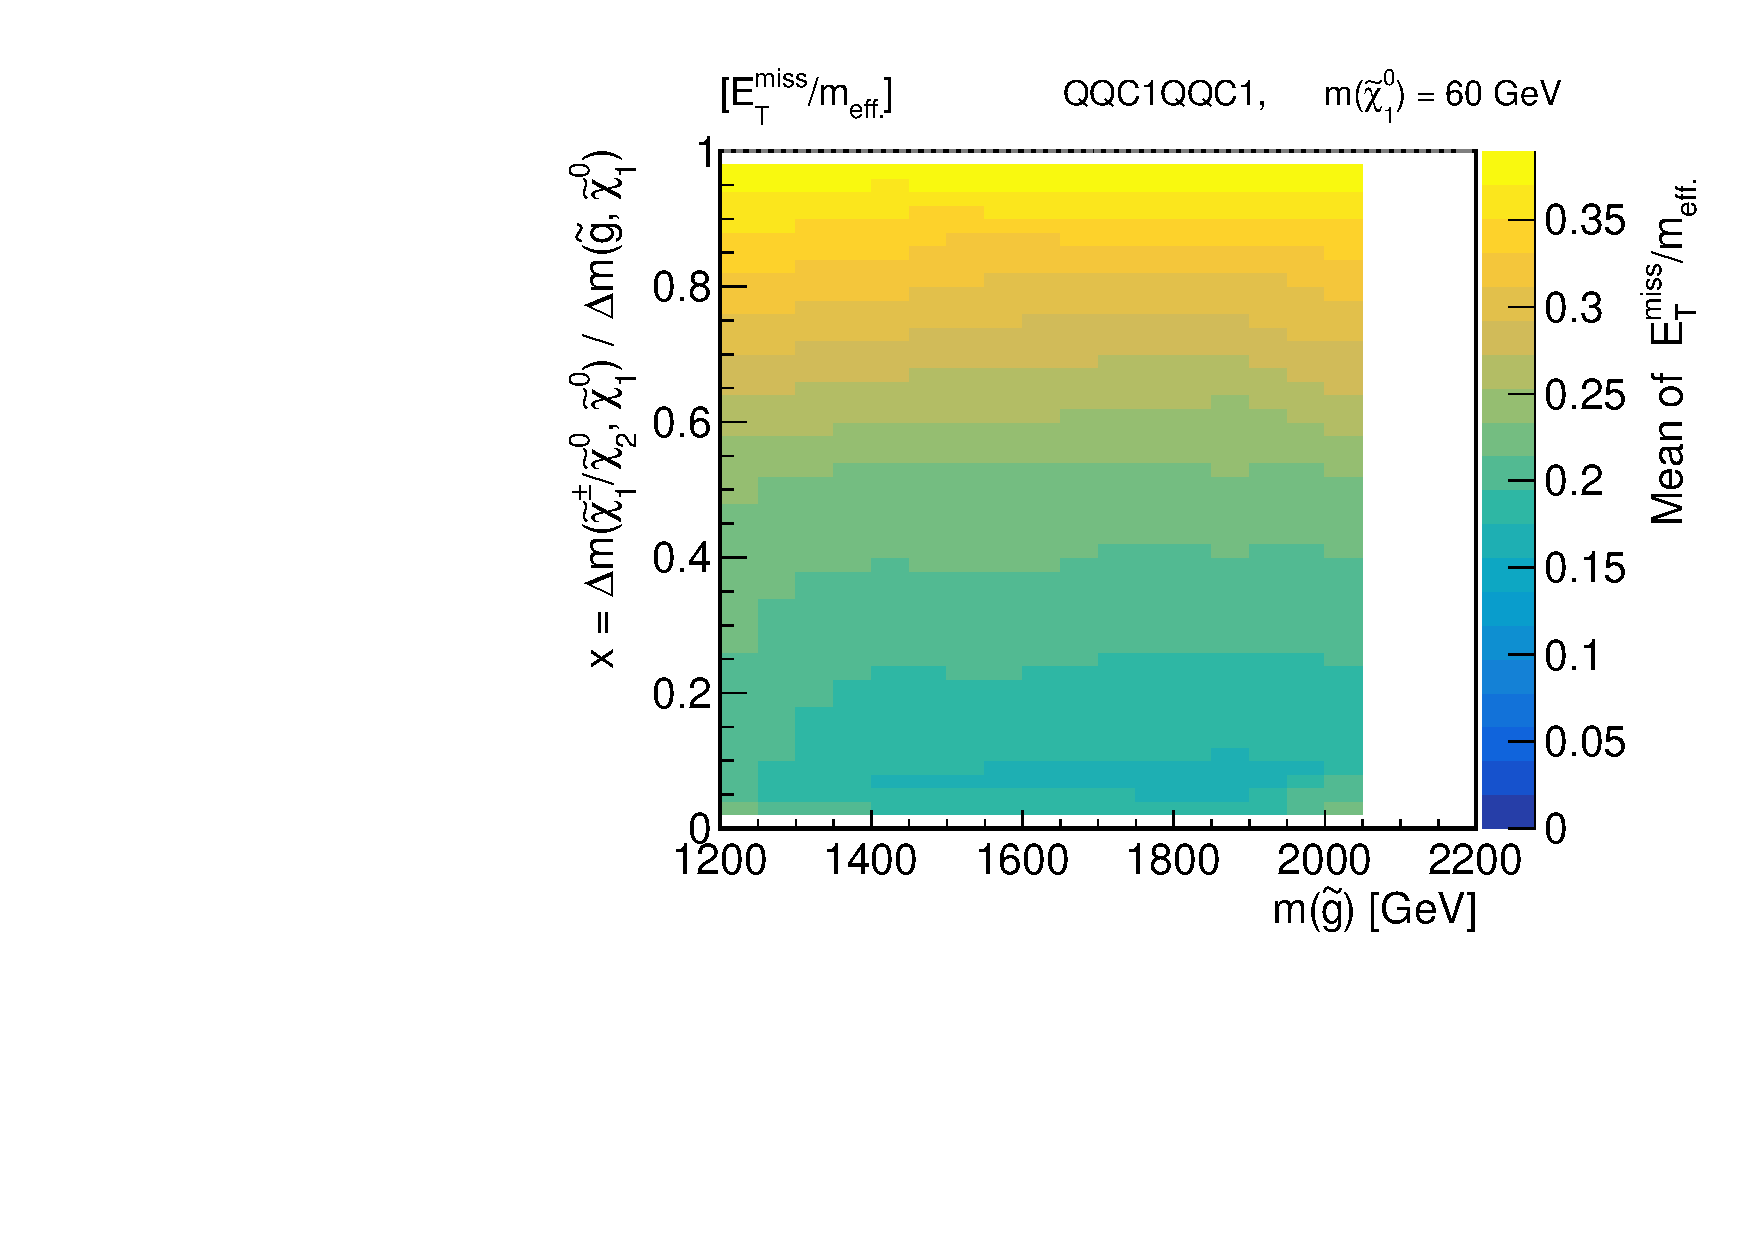
\includegraphics[width=0.45\textwidth]{figures/SRdefinition/kineMap/GG_symQQC1_varx_metOverMeff.pdf}}
    \subfigure[]{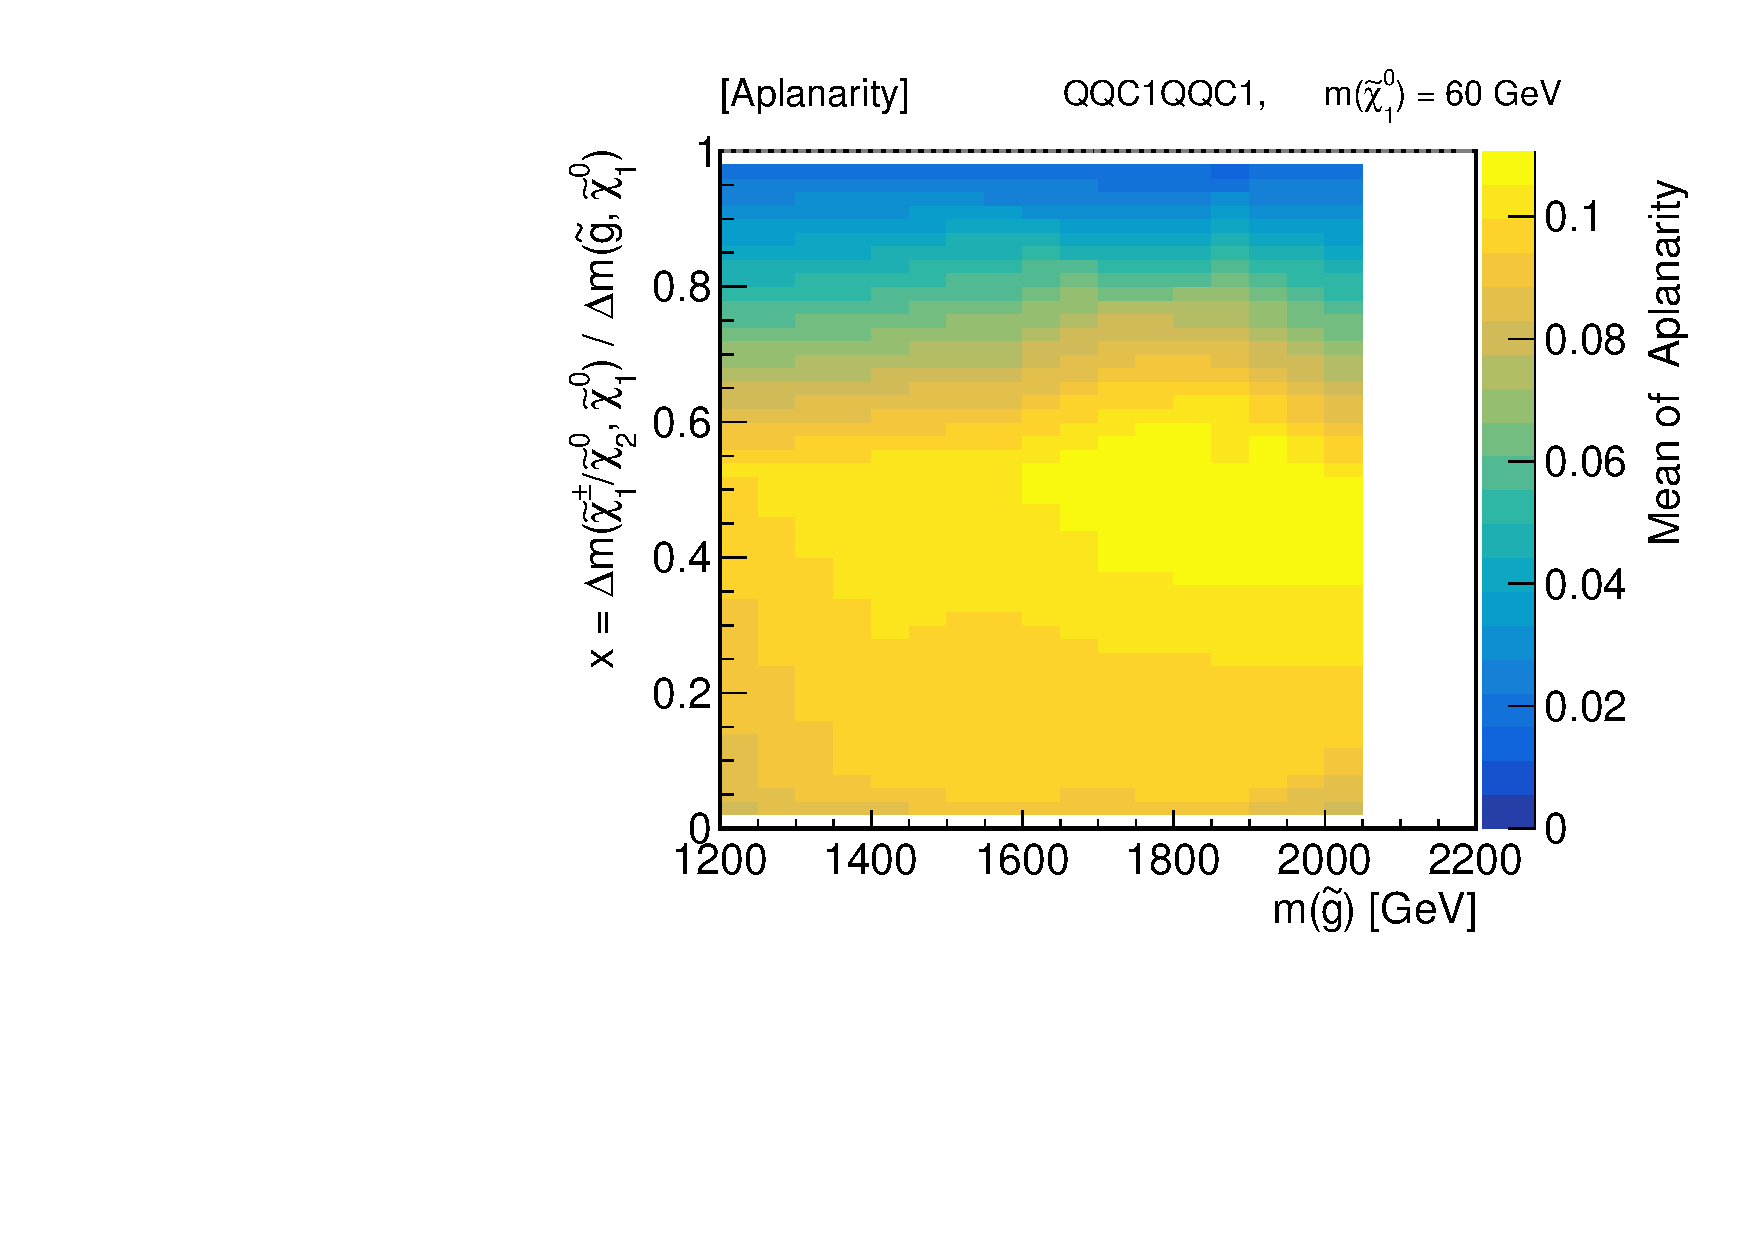
\includegraphics[width=0.45\textwidth]{figures/SRdefinition/kineMap/GG_symQQC1_varx_LepAplanarity.pdf}}
    \caption{ Mean of (a) $\meffInc$ (b) $\met$ (c) $\lepPt$ (d) $\mt$ (e) $\metOverMeff$  (f) aplanarity, for the QQC1QQC1 \varx grid, after the pre-selection. 
      \label{fig::SRdefinition::kineMap_QQC1QQC1_varx} 
    }
\end{figure}

 
%\begin{figure}[h]
%  \centering
%    \subfigure[]{\includegraphics[width=0.45\textwidth]{figures/SRdefinition/kineMap/GG_symQQC1_dM20_nJet30.pdf}}
%    \subfigure[]{\includegraphics[width=0.45\textwidth]{figures/SRdefinition/kineMap/GG_symQQC1_dM20_meff.pdf}}
%    \subfigure[]{\includegraphics[width=0.45\textwidth]{figures/SRdefinition/kineMap/GG_symQQC1_dM20_met.pdf}}
%    \subfigure[]{\includegraphics[width=0.45\textwidth]{figures/SRdefinition/kineMap/GG_symQQC1_dM20_lep1Pt.pdf}}
%    \subfigure[]{\includegraphics[width=0.45\textwidth]{figures/SRdefinition/kineMap/GG_symQQC1_dM20_mt.pdf}}
%    \subfigure[]{\includegraphics[width=0.45\textwidth]{figures/SRdefinition/kineMap/GG_symQQC1_dM20_LepAplanarity.pdf}}
%    \caption{ Mean of (a) jet-multiplicity ($p_T>30\gev$) (b) $\meffInc$ (c) $\met$ (d) $\lepPt$ (e) $\mt$ (f) aplanarity, for the QQC1QQC1 $\Delta M = 20\gev$ grid, after the pre-selection. }
%\end{figure}
 
\begin{figure}[h]
  \centering
%    \subfigure[]{\includegraphics[width=0.45\textwidth]{figures/SRdefinition/kineMap/GG_symQQC1_dM30_nJet30.pdf}}
    \subfigure[]{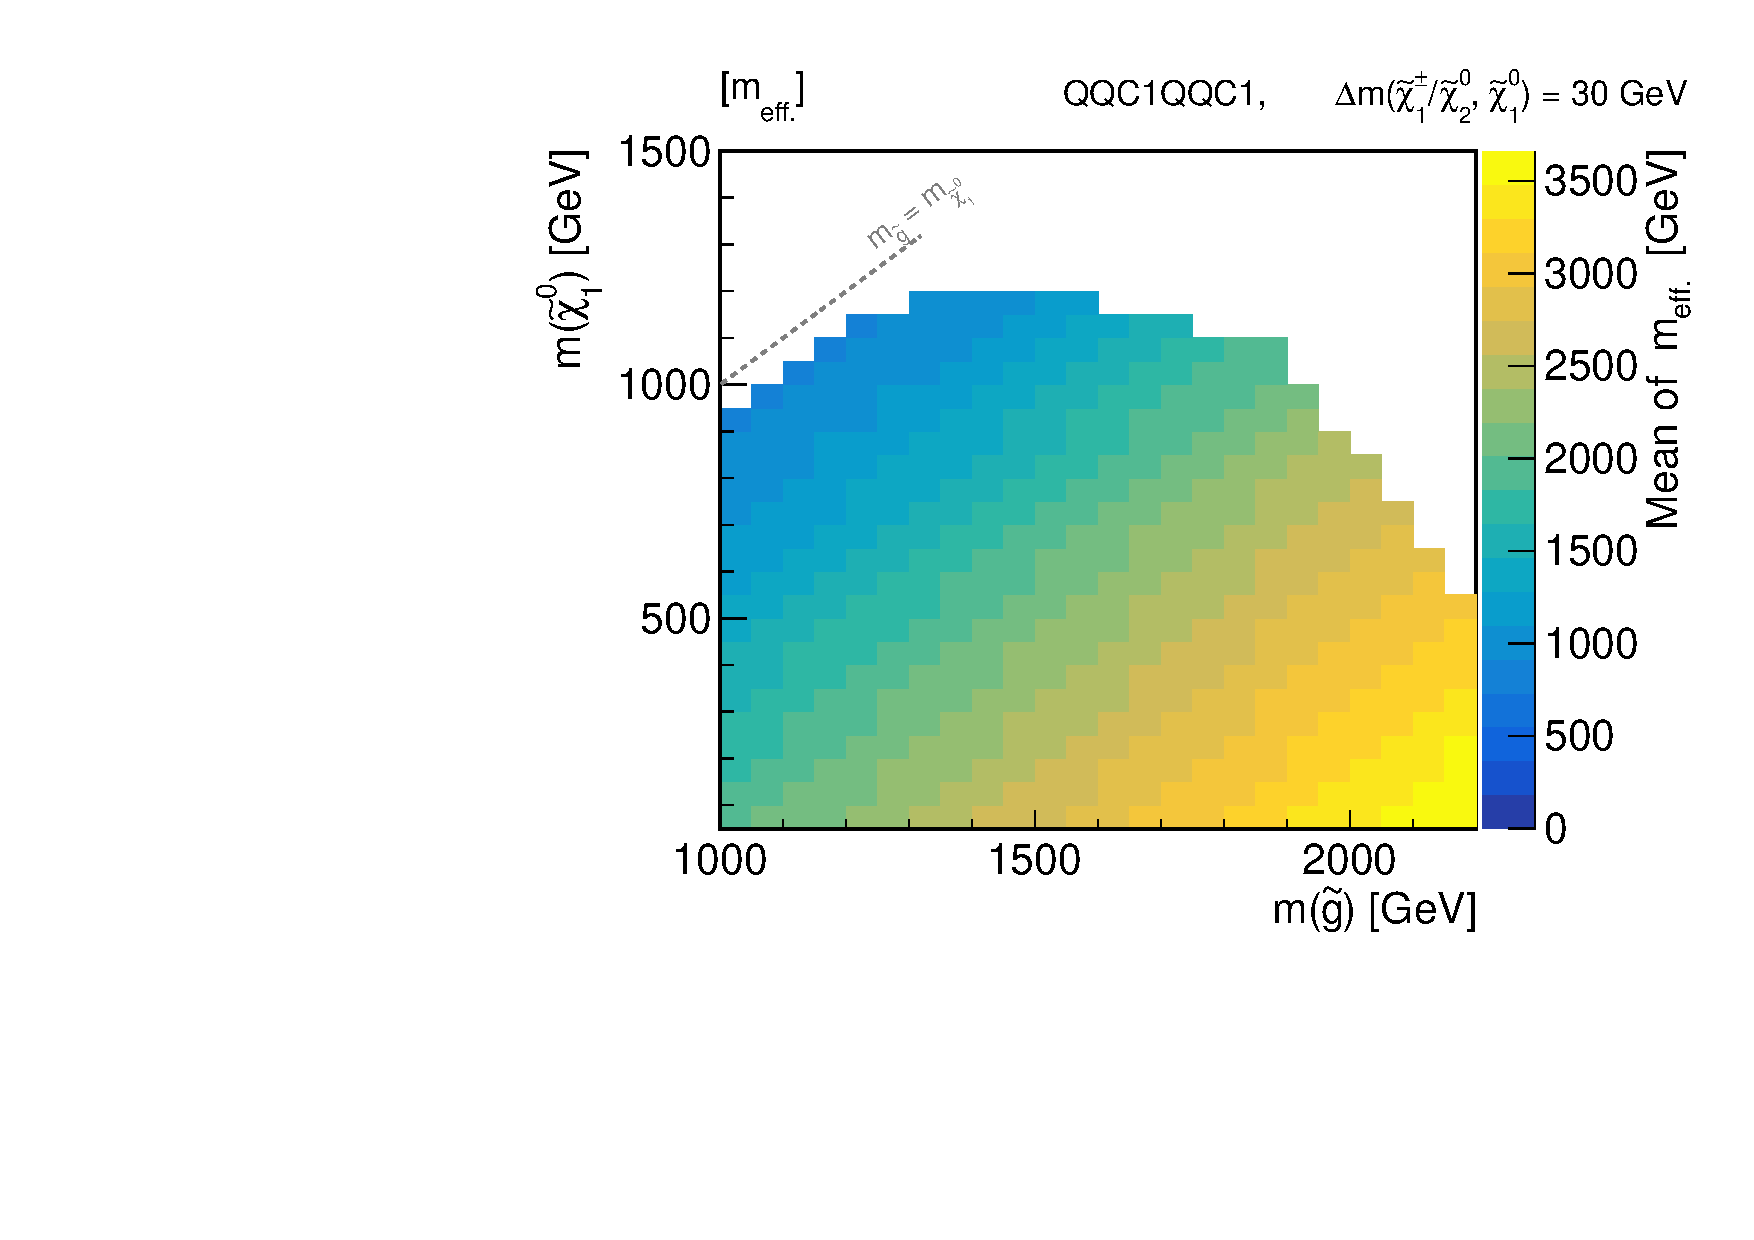
\includegraphics[width=0.45\textwidth]{figures/SRdefinition/kineMap/GG_symQQC1_dM30_meff.pdf}}
    \subfigure[]{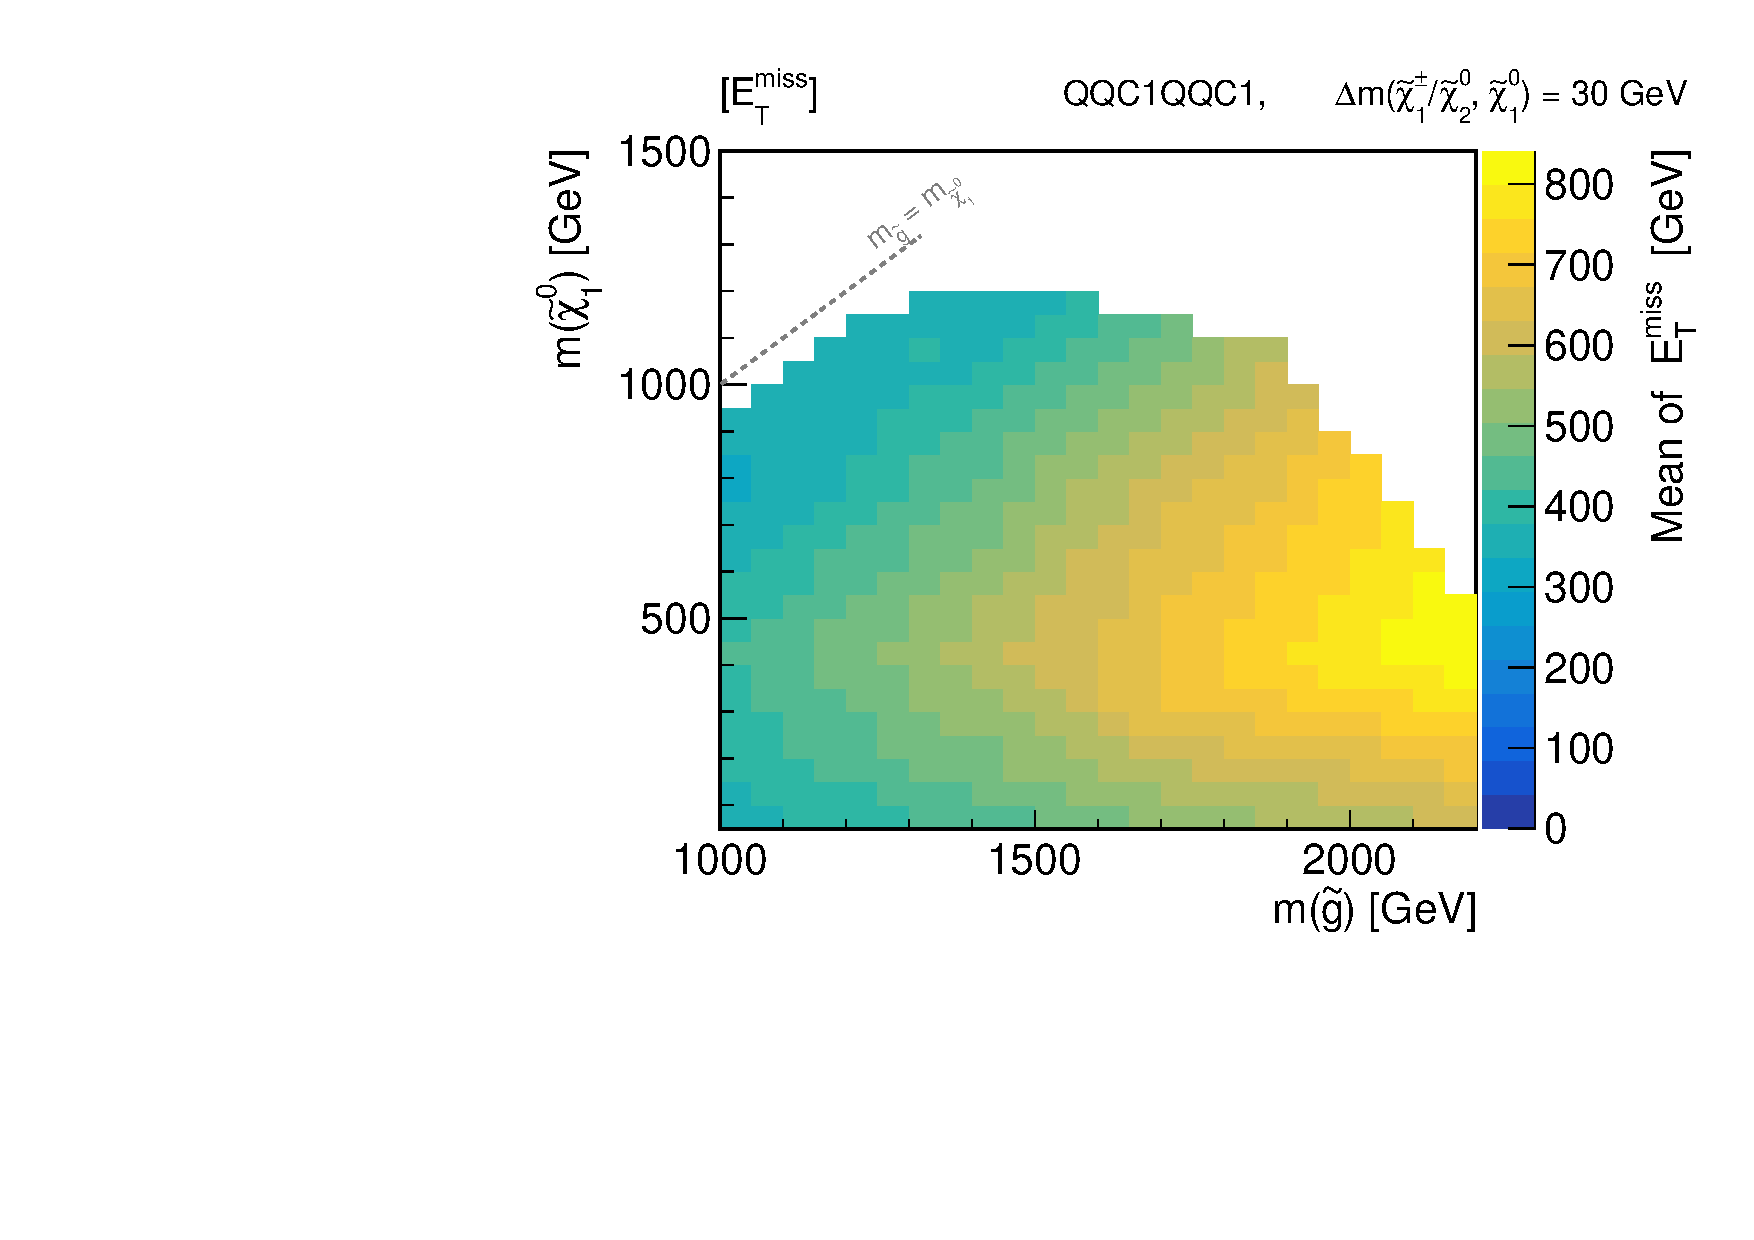
\includegraphics[width=0.45\textwidth]{figures/SRdefinition/kineMap/GG_symQQC1_dM30_met.pdf}}
    \subfigure[]{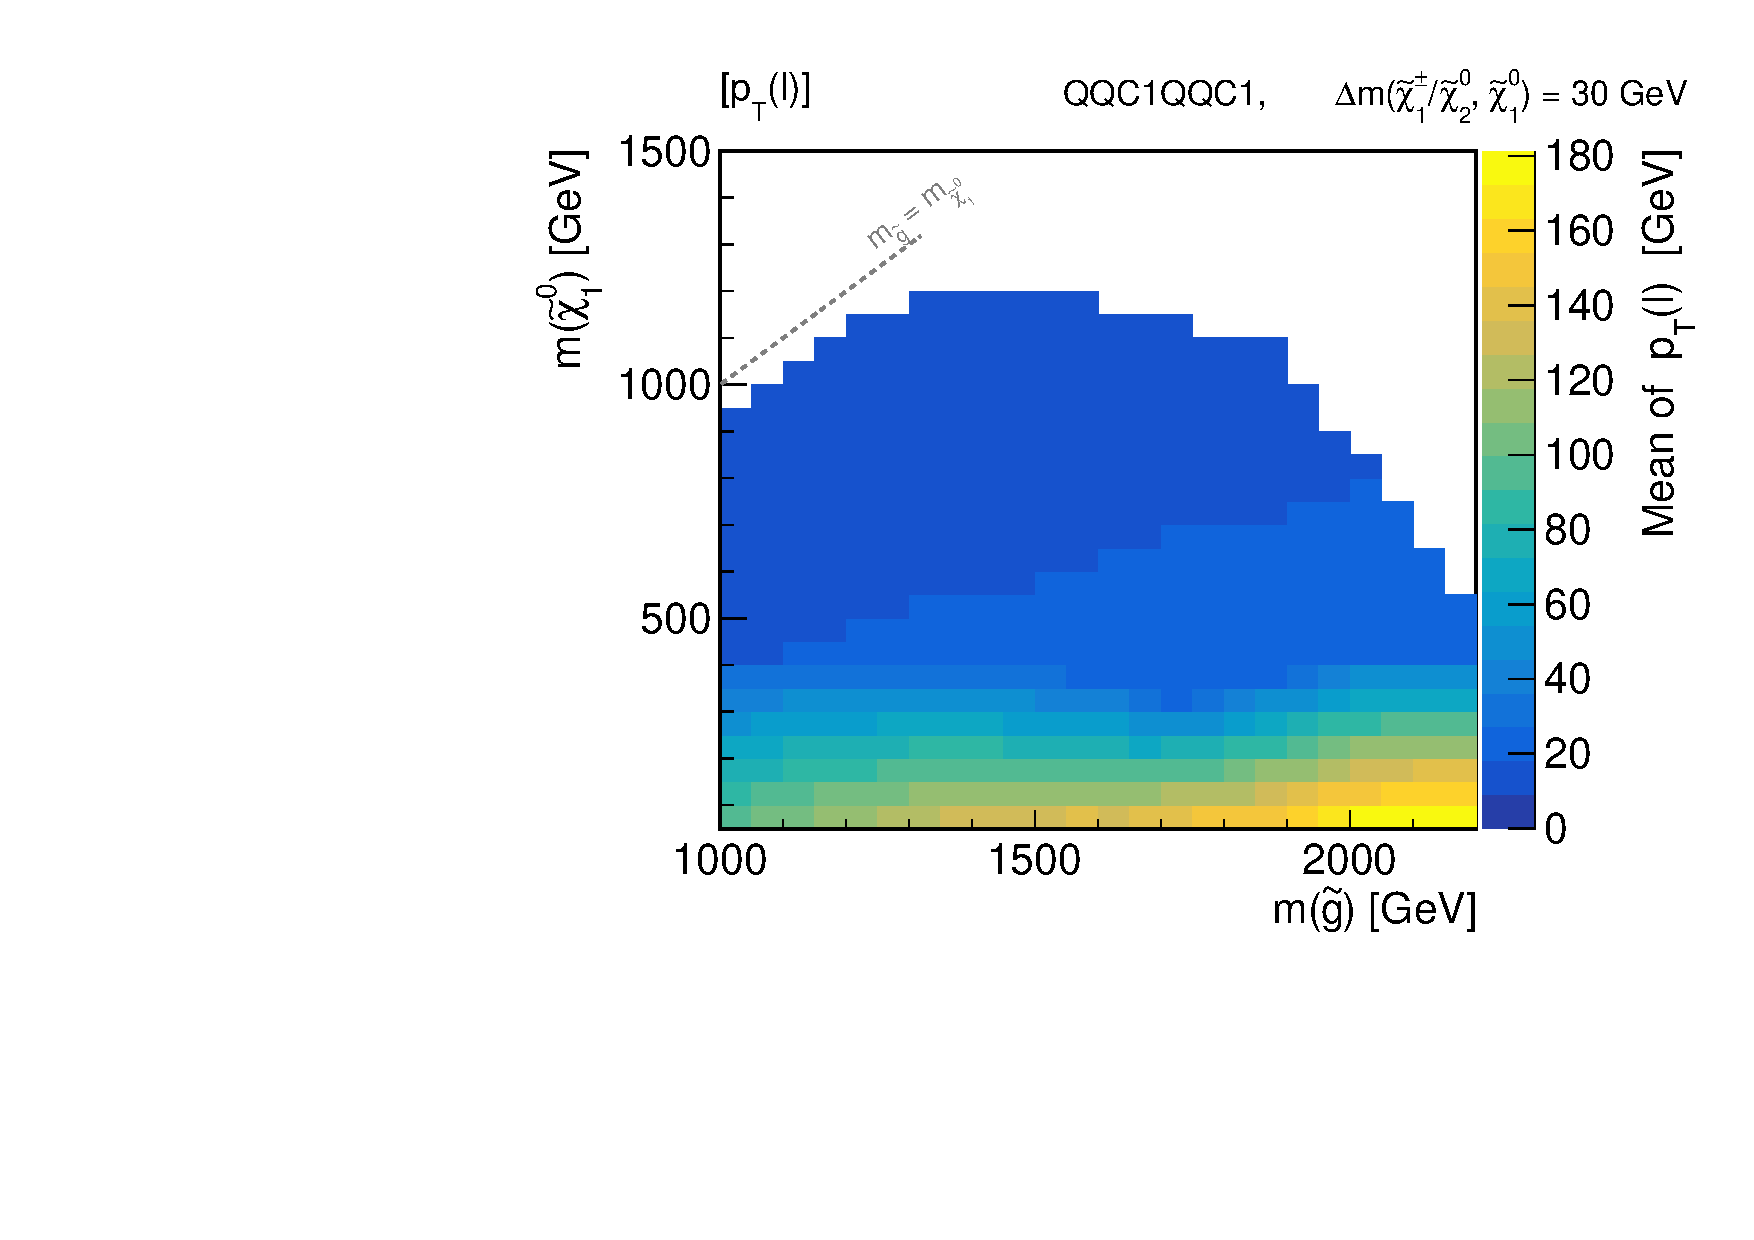
\includegraphics[width=0.45\textwidth]{figures/SRdefinition/kineMap/GG_symQQC1_dM30_lep1Pt.pdf}}
    \subfigure[]{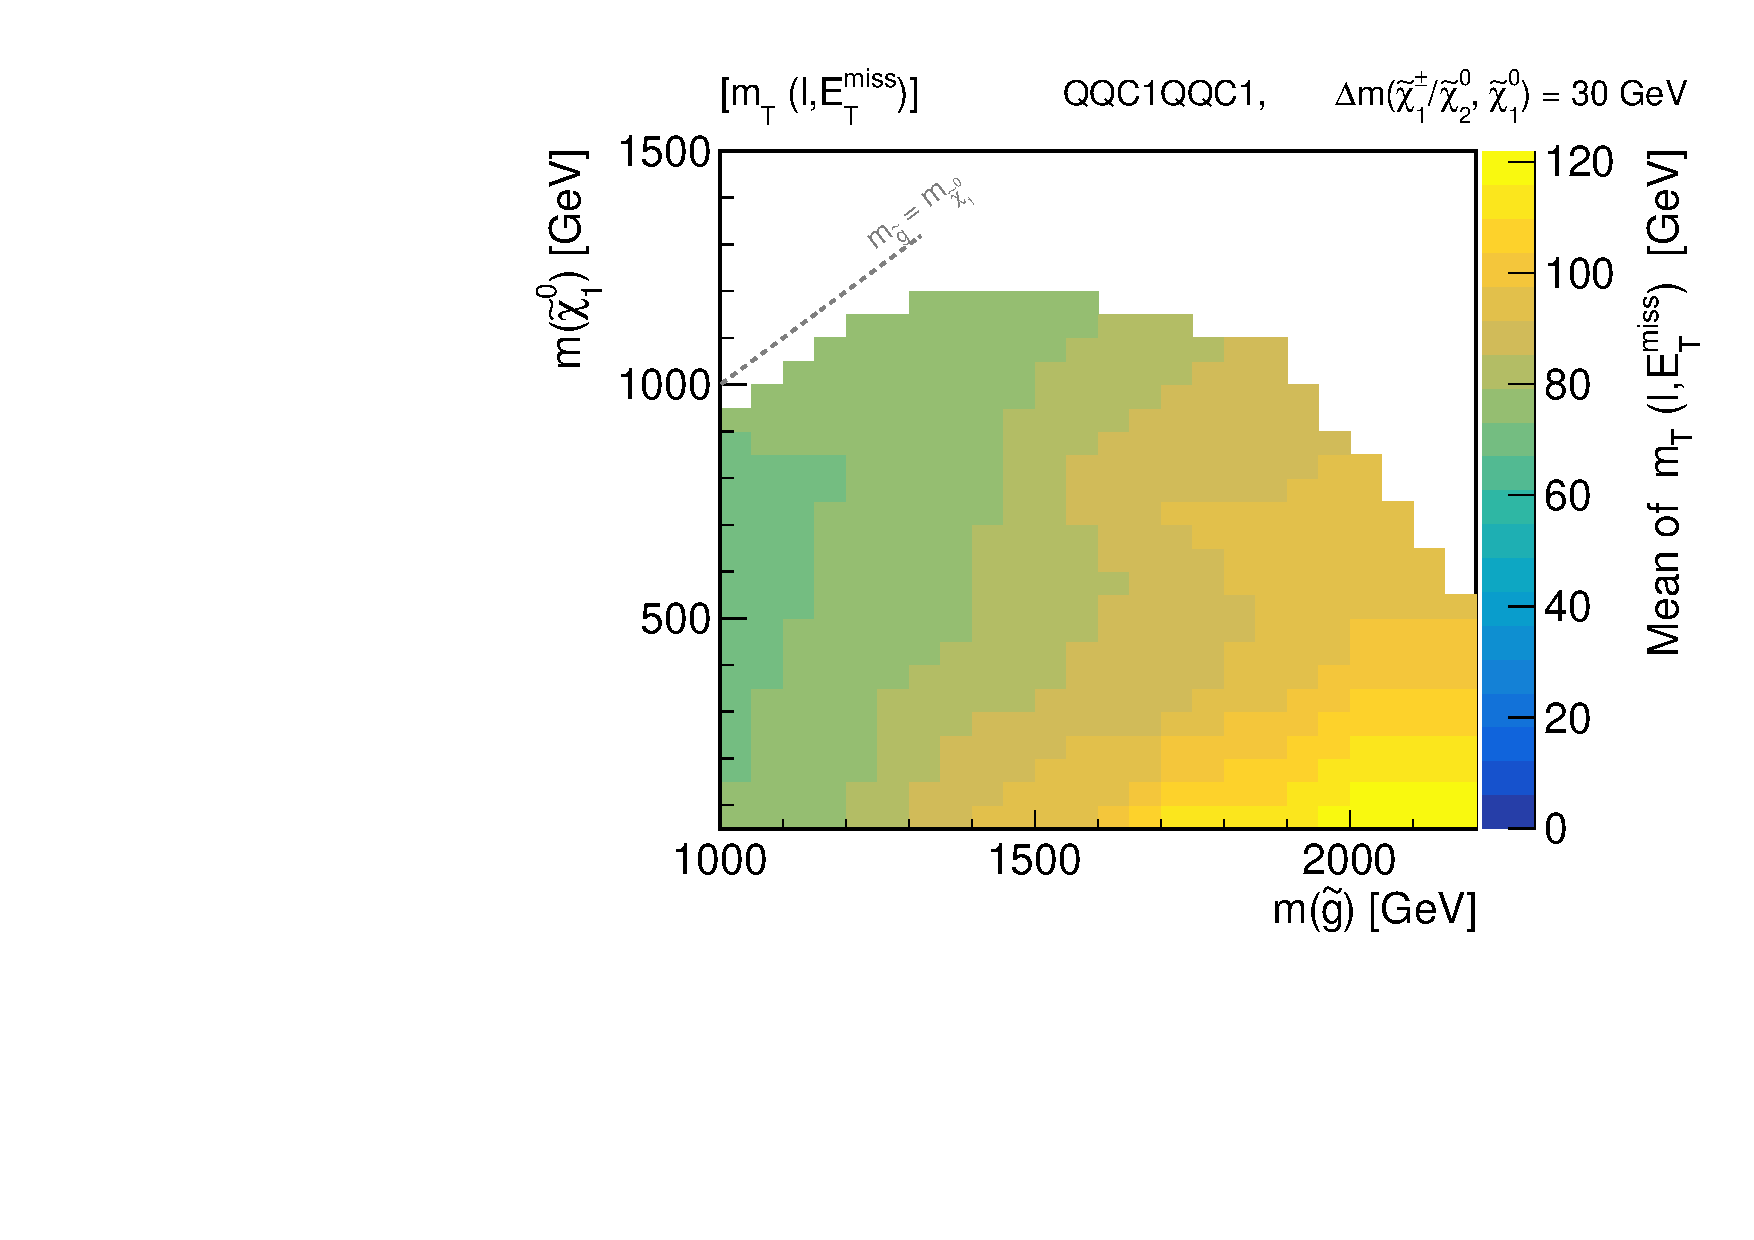
\includegraphics[width=0.45\textwidth]{figures/SRdefinition/kineMap/GG_symQQC1_dM30_mt.pdf}}
    \subfigure[]{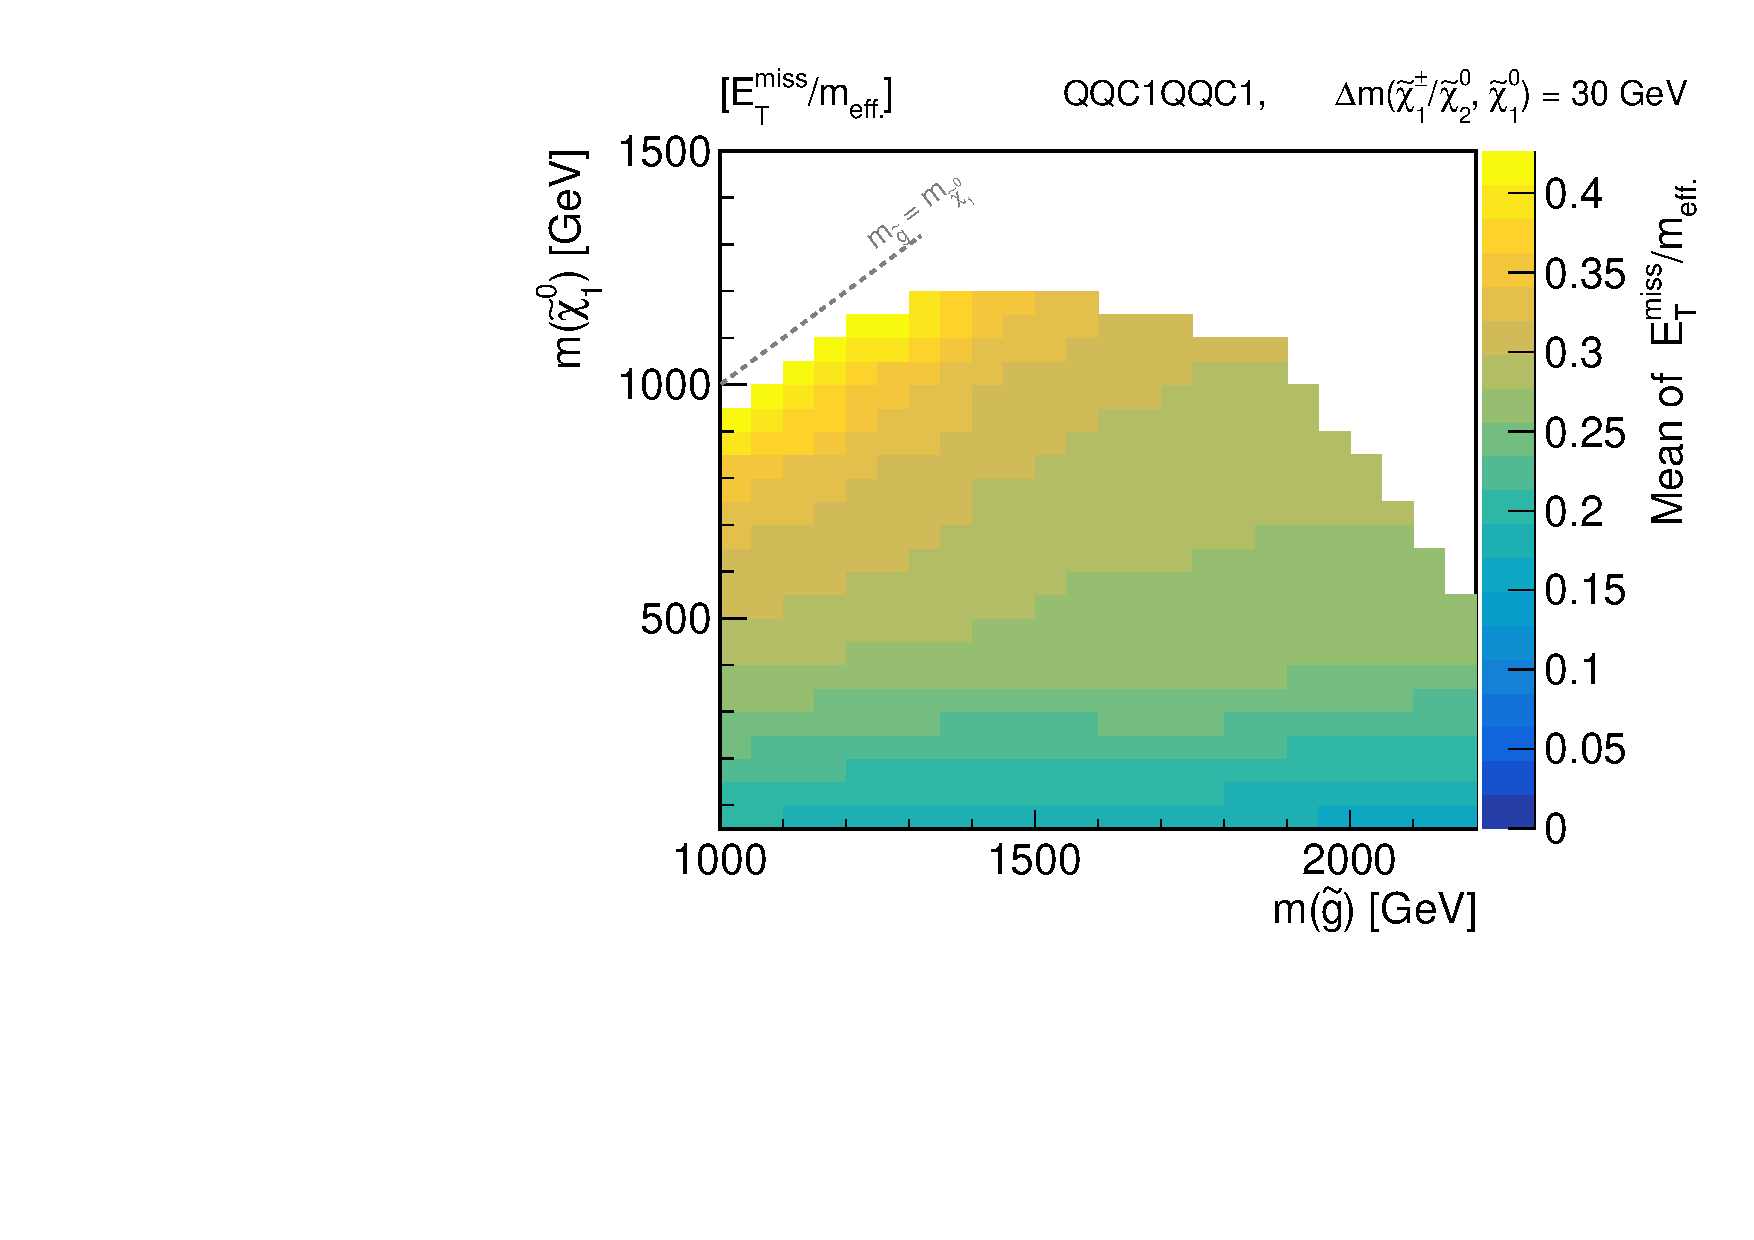
\includegraphics[width=0.45\textwidth]{figures/SRdefinition/kineMap/GG_symQQC1_dM30_metOverMeff.pdf}}
    \subfigure[]{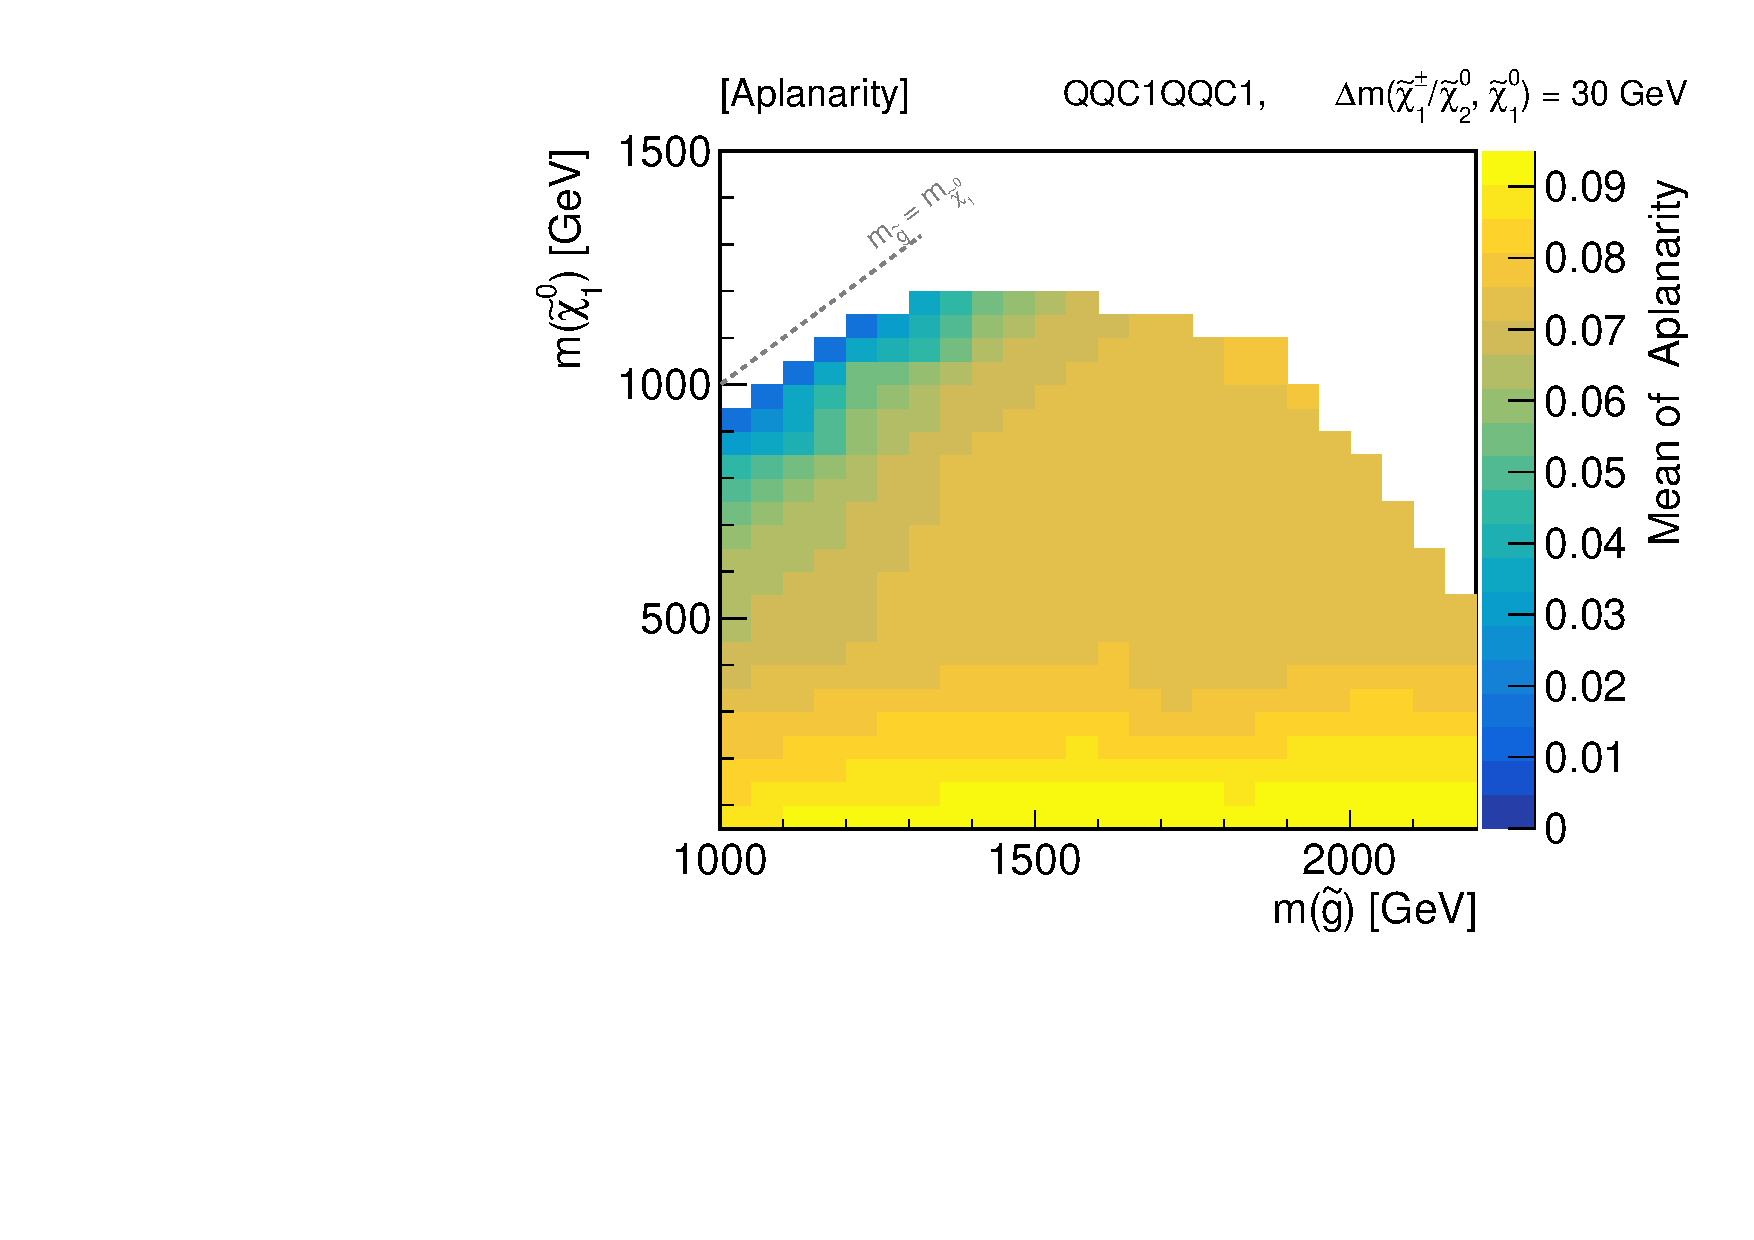
\includegraphics[width=0.45\textwidth]{figures/SRdefinition/kineMap/GG_symQQC1_dM30_LepAplanarity.pdf}}
    \caption{ Mean of (a) $\meffInc$ (b) $\met$ (c) $\lepPt$ (d) $\mt$ (e) $\metOverMeff$ (f) aplanarity, for the QQC1QQC1 \DMth grid, after the pre-selection. 
      \label{fig::SRdefinition::kineMap_QQC1QQC1_dM30} 
    }
\end{figure}


\begin{figure}[h]
  \centering
    \subfigure[]{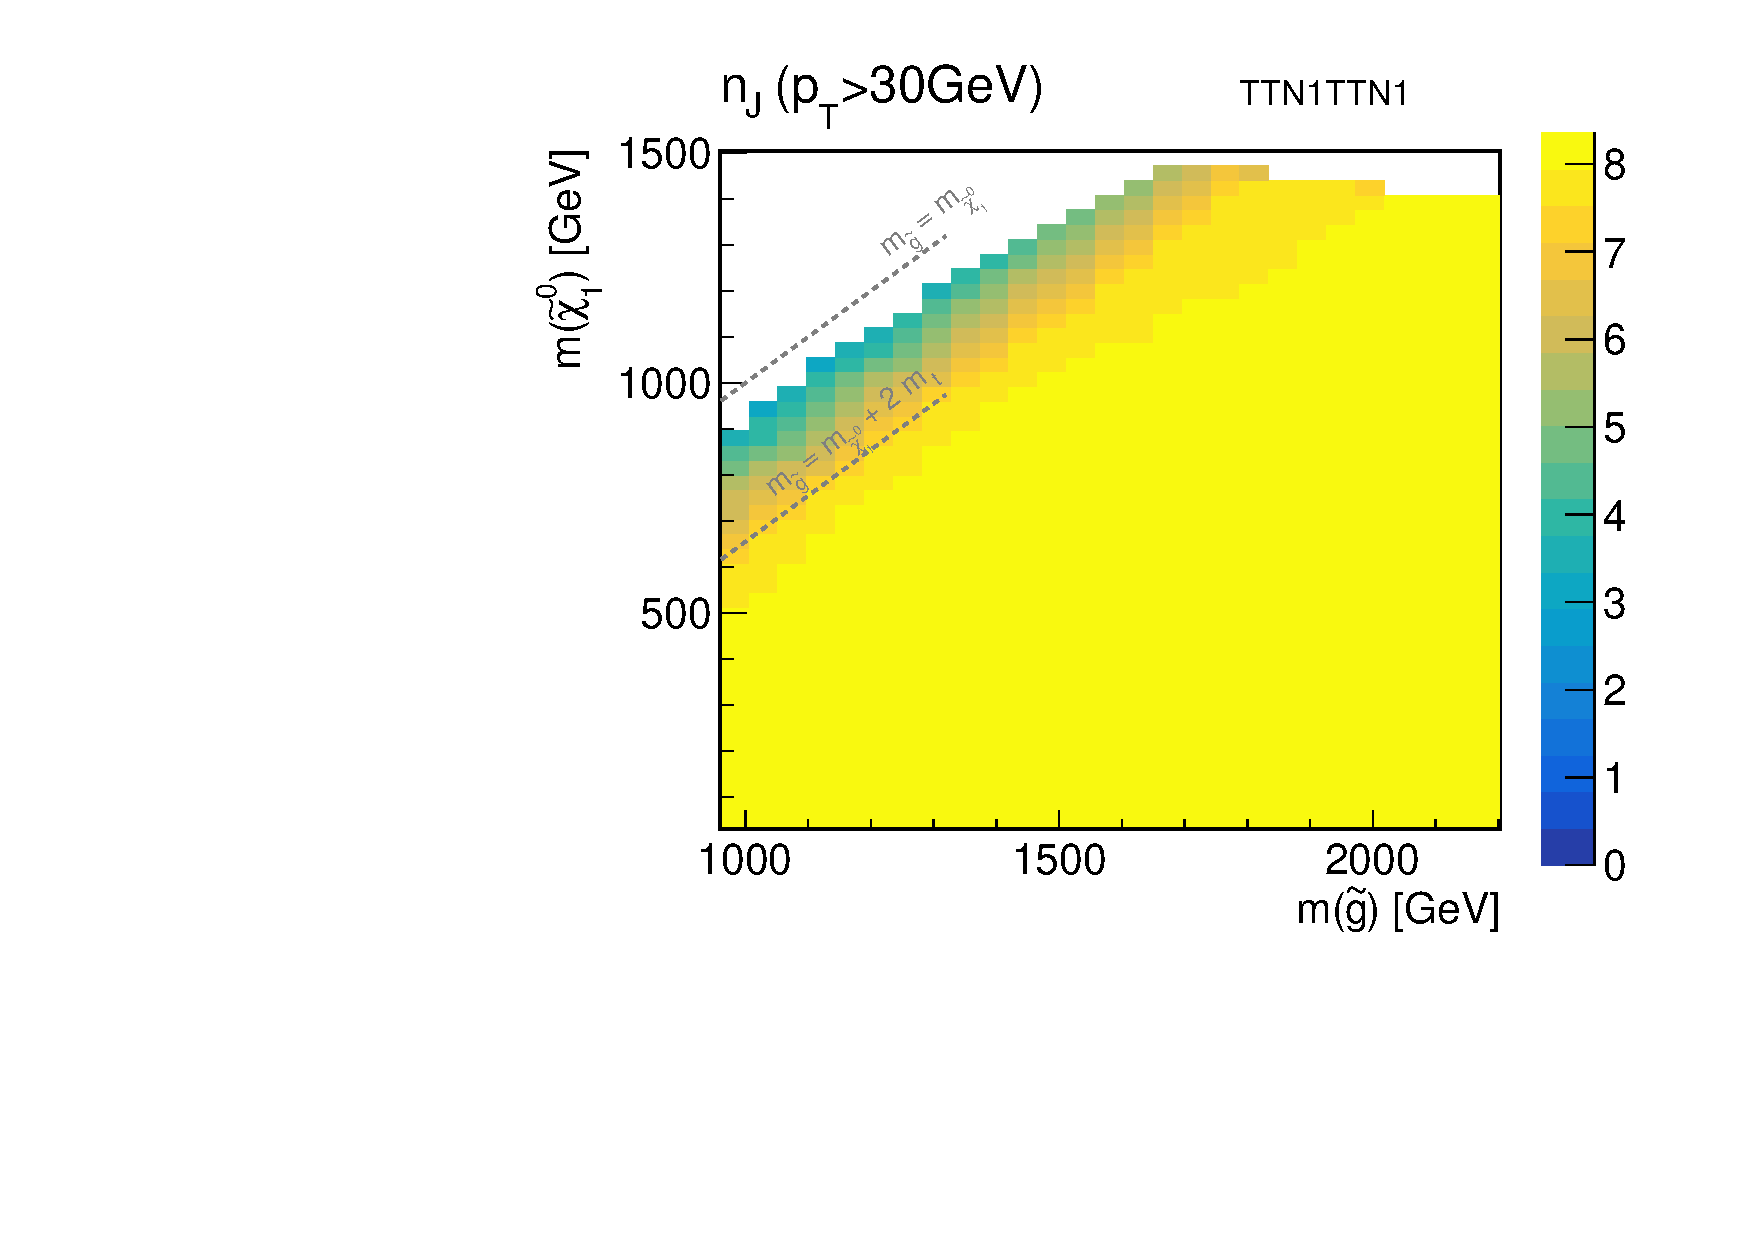
\includegraphics[width=0.32\textwidth]{figures/SRdefinition/kineMap/GG_symTTN1_x12_nJet30.pdf}}
    \subfigure[]{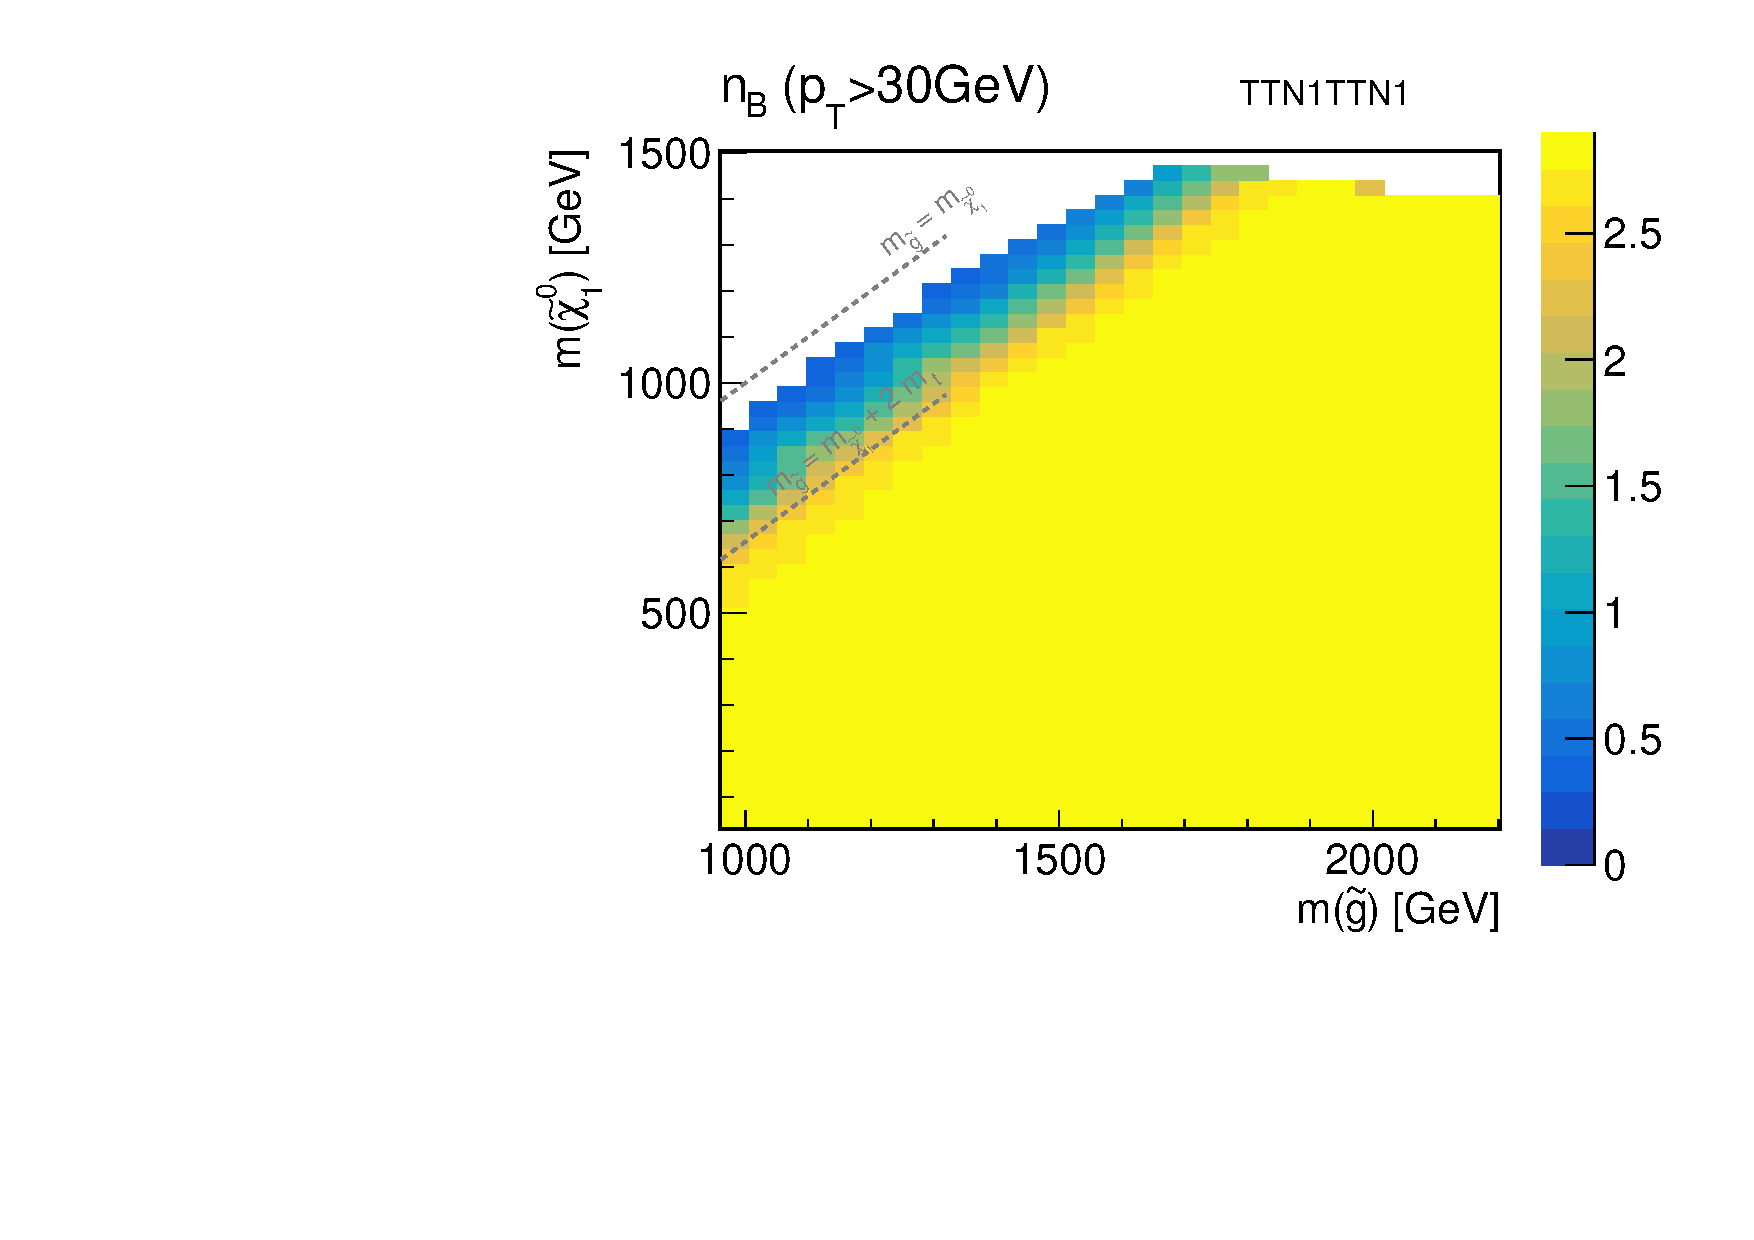
\includegraphics[width=0.32\textwidth]{figures/SRdefinition/kineMap/GG_symTTN1_x12_nBJet30.pdf}}
    \subfigure[]{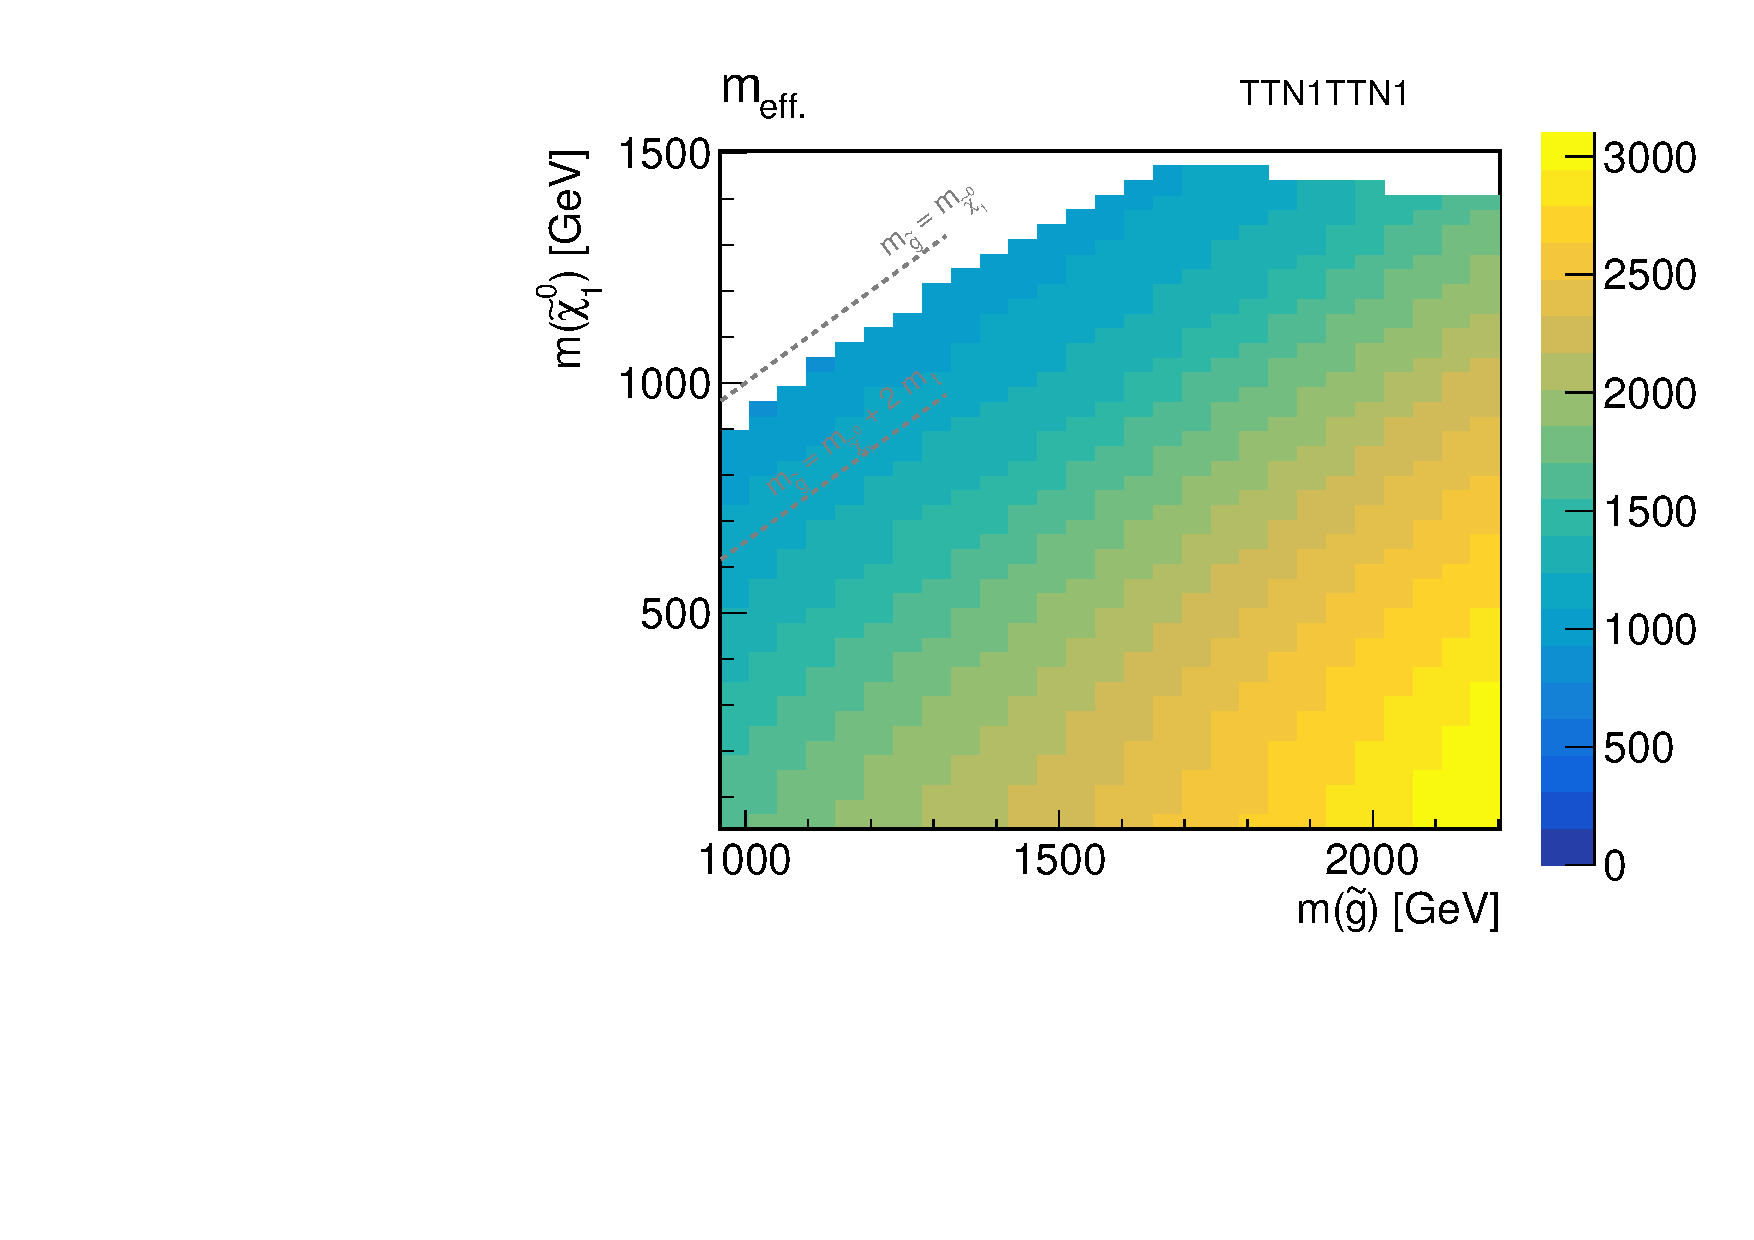
\includegraphics[width=0.32\textwidth]{figures/SRdefinition/kineMap/GG_symTTN1_x12_meff.pdf}}
    \subfigure[]{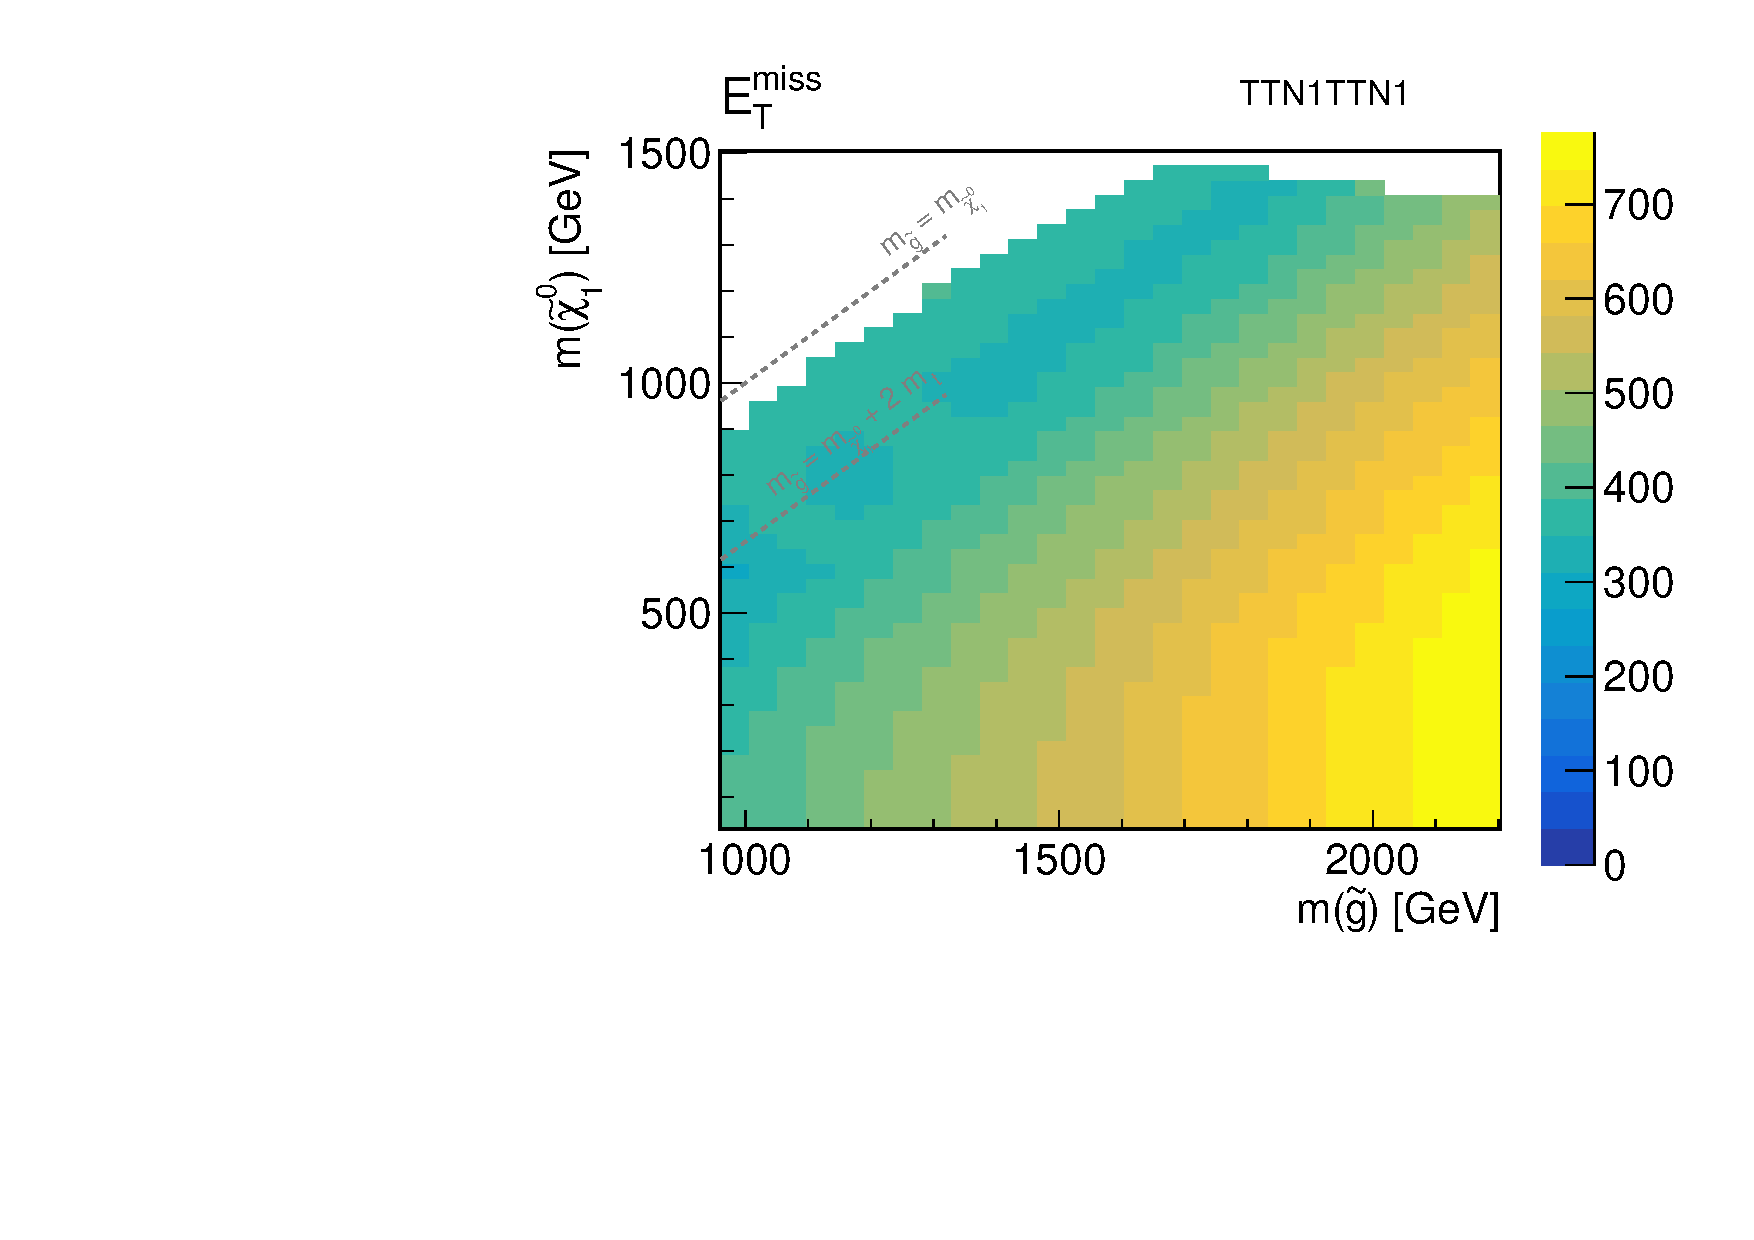
\includegraphics[width=0.32\textwidth]{figures/SRdefinition/kineMap/GG_symTTN1_x12_met.pdf}}
    \subfigure[]{\includegraphics[width=0.32\textwidth]{figures/SRdefinition/kineMap/GG_symTTN1_x12_lep1Pt.pdf}}
    \subfigure[]{\includegraphics[width=0.32\textwidth]{figures/SRdefinition/kineMap/GG_symTTN1_x12_mt.pdf}}
    \subfigure[]{\includegraphics[width=0.32\textwidth]{figures/SRdefinition/kineMap/GG_symTTN1_x12_LepAplanarity.pdf}}
    \subfigure[]{\includegraphics[width=0.32\textwidth]{figures/SRdefinition/kineMap/GG_symTTN1_x12_min_dPhi_4j.pdf}}
    \subfigure[]{\includegraphics[width=0.32\textwidth]{figures/SRdefinition/kineMap/GG_symTTN1_x12_topNess.pdf}}
    \caption{ Mean of (a) jet-multiplicity ($p_T>30\gev$) (b) bjet-multiplicity ($p_T>30\gev$) (c) $\meffInc$ (d) $\met$ (e) $\lepPt$ (f) $\mt$ (g) aplanarity (h) $\mindPhiFourJet$ (i) topness, for the TTN1TTN1 \dire grid, after the pre-selection. 
      \label{fig::SRdefinition::kineMap_TTN1TTN1} 
    }
\end{figure}
 


%%%%%%%%%%%%%%%%%%%%%%%%%%%%%%%%%%%%%
\clearpage		
\subsubsection{Cut Optimization}
The cut values for the kinematic variables listed above are optimized, including the lower $\meffInc$ cut for the highest $\meffInc$-bin. Reference signal points are defined in Tab. \ref{tab::SRdefinition::refSigPointsOptm}, to which the sensitivity is optimized. The optimization procedure proceeds as following.

\begin{enumerate}
\item The binning of $\meffInc$ is roughly decided so that the sensitivities for all the reference points in the same tower are maintained.
\item Cuts values in other variables are then optimized by a simultaneous grid scan using machinary. The initial values are chosen based on the target mass regions of each signal region (as depicted by Fig. \ref{fig::SRdefinition::towerCoverage1}-Fig. \ref{fig::SRdefinition::towerCoverage2}), and the typical kinematics of such signals as shown in Fig. \ref{fig::SRdefinition::kineMap_QQC1QQC1_x12}-\ref{fig::SRdefinition::kineMap_TTN1TTN1}.
The sensitivity as the reference of the optimizaton is defined by the combined significance of $\meffInc$ bins such as :
\begin{align}
& Z_{N,\mathrm{comb.}} =\sqrt{\sum_i Z_{N,i}^2}, \nn \\
& Z_{N,i} := S_i/\sqrt{B_i+\alpha^2 B_i^2}, \label{ZNcomb}
\end{align}
where $Z_{N,i}$ is the significance provided by a single $\meffInc$ bin, with $S_i$, $B_i$ being the signal and background yields in the $\meffInc$ bin. $\alpha$ is the parameter representing the systematics uncertainty on background estimation in the $\meffInc$ bin, where flat $30\%$ is assigned during the optimization. The cut between BT and BV bins in the same tower and $\meffInc$-bin are always set to common.

\item All the cuts including the $\meffInc$ binning are re-optimized by pertubating them from the optimum configuration obtained in the previous step simultaneously.

\item Optimum cuts are different bewteen reference points in the same $\meffInc$ tower. An adjustment is therefore applied for the best compromisation, as well as to avoid the over-optimization on specific signal points.

\item Another minor adjustment is done afterwards, required from the context of background estimation. Some of the cuts are loosened to facilitate the control region definition.
\end{enumerate}

\tab{ c c c}{
      \hline
      &   Model    & $(\mG,\mC,\mLSP)$,$(\mG,\mLSP)$ [GeV] \\
      \hline
      \hline
      \textbf{2J BV}  & & \\
      \hline
      &   QQC1QQC1 & (1550,580,550)  \\
      &   QQC1QQC1 & (1065,1025,985) \\
      &   TTN1TTN1 & (1000,915)      \\
      \hline
      \textbf{2J BT}  & & \\
      \hline
      &   QQC1BTC1 & (1400,830,800)  \\
      &   QQC1BTC1 & (1550,780,750)  \\
      \hline
      \textbf{6J BV}  & & \\
      \hline
      &  QQC1QQC1 & (1945,1105,265)  \\
      &  QQC1QQC1 & (1850,1350,850)  \\
      &  QQC1QQC1 & (1700,1300,900)  \\
      \hline
      \textbf{6J BT}  & & \\
      \hline
      &  QQC1BTC1 & (1850,1050,250) \\
      &  QQC1BTC1 & (1700,1300,900)  \\ 
      \hline
      \textbf{Low-x BV}  & & \\
      \hline
      &  QQC1QQC1 & (1700,460,60)    \\ 
      &  QQC1QQC1 & (1600,260,60)    \\
      &  QQC1QQC1 & (1700,530,500)     \\                                
      \hline
      \textbf{Low-x BT}  & & \\
      \hline
      &  QQC1BTC1 & (1700,730,700) \\
      &  QQC1BTC1 & (1700,530,500) \\
      \hline
      \textbf{High-x BV}  & & \\
      \hline
      &  QQC1QQC1 & (1800,1600,60) \\
      &  QQC1QQC1 & (1800,1460,60) \\
      &  QQC1QQC1 & (1800,1260,60) \\
      \hline
      \textbf{High-x BT} & & \\
      \hline
      &  QQC1BTC1 & (1850,1750,60)    \\
      &  QQC1BTC1 & (1850,1450,60)    \\
      \hline
      \textbf{3B}  & & \\
      \hline
      &  TTN1TTN1 &  (2000,0)     \\ 
      &  TTN1TTN1 &  (1900,800)   \\ 
      &  TTN1TTN1 &  (1500,1000)   \\
      \hline
}
{The reference signal points for each signal regions to which the selection is optimized to.}
{tab::SRdefinition::refSigPointsOptm}


Finalized definition of signal regions are shown in Tab. \ref{SRdefinition::regionDef2J}-\ref{SRdefinition::regionDef3B}. The $\meffInc$ distribution in the optimized signal regions are displayed in Fig. \ref{fig::SRdefinition::SRmeffInc2J}-\ref{fig::SRdefinition::SRmeffInc3B} for backgrounds with the reference signal points overlaid. The segmentation of $\meffInc$-bin is found to successfully address the sensitivity in different mass region in the signal grid. \\

The optimized selection is also validated by a set looking at the kinematic distribution Fig. \ref{fig::SRdefinition::N1plots_2JMEFFInclBV}-\ref{fig::SRdefinition::N1plots_3BMEFFIncl} in which the one of the cuts is loosened from the optimized signal regions. The sensitivity is calculated as function of the cut position of the removed cut. The decided cuts are shown by the red arrows, which are more or less at the optimum position for all the reference signals.


			%%%%%%%%  2J  %%%%%%%%%%%%
			\renewcommand{\arraystretch}{1.8}
			\tab{ c | c c c c c c}{
			                             \hline
                                             &            SR (BV/BT) &                 WR/TR &             VR $\met$ &               VRb &                VR QCD &                 VR DB \\ \hline
                                 $\nLepbase$ &                     1 &                     1 &                     1 &                     1 &                     1 &                     2 \\
                               $\nLepsignal$ &                     1 &                     1 &                     1 &                     1 &                     0 &                     2 \\
                                    $\lepPt$ & \multicolumn{5} {c}{                                                                                      $[6,35]$ } &                     - \\
                                     $\nJet$ & \multicolumn{5} {c}{                                                                                       $\geq2$ } &               $\geq1$ \\
                                    $\nBJet$ &               0/[1,2] &               0/[1,2] &                     - &                     - &                     - &                     0 \\
                                      $\met$ &                $>430$ &           $[250,430]$ &           $[250,430]$ &                $>430$ &                $>430$ &                $>250$ \\
                                  $\meffInc$ & \multicolumn{6} {c}{                                                                        $[1100,1500], \,\,[1500,1900], \,\,>1900$ } \\
                                   $\mtFull$ &                $>100$ &            $[30,100]$ &                $>100$ &            $[30,100]$ &                $>100$ &                     - \\
                              $\metOverMeff$ &               $>0.25$ &               $>0.15$ &                $>0.1$ &                $>0.2$ &               $>0.25$ &                     - \\
                            $\nJetOverLepPt$ & \multicolumn{2} {c}{                $>0.2$ } &               $>0.15$ & \multicolumn{2} {c}{                $>0.2$ } &                     - \\
                                  $\topNess$ &                  $>4$ &                     - &                     - &                  $>4$ &                  $>4$ \\
			  \hline }
			{Definition of signal/control/validation regions (SRs/CRs/VRs) for tower \textbf{"2J"}}
			{SRdefinition::regionDef2J}
			\renewcommand{\arraystretch}{1.}



			%%%%%%%%  6J  %%%%%%%%%%%%
			\renewcommand{\arraystretch}{1.8}
			\tab{ c | c c c c c c}{
			                             \hline
                                             &            SR (BV/BT) &                 WR/TR &              VRa &               VRb &                VR QCD &                 VR DB \\ \hline
                                 $\nLepbase$ &                     1 &                     1 &                     1 &                     1 &                     1 &                     2 \\
                               $\nLepsignal$ &                     1 &                     1 &                     1 &                     1 &                     0 &                     2 \\
                                    $\lepPt$ & \multicolumn{6} {c}{                                                                                                                 $>35$ } \\
                                     $\nJet$ & \multicolumn{5} {c}{                                                                                       $\geq6$ } &               $\geq5$ \\
                                    $\nBJet$ &               0/[1,2] &               0/[1,2] &                     - &                     - &                     - &                     0 \\
                                      $\met$ &                $>350$ &                $>300$ &                $>250$ &                $>350$ &                $>350$ &                $>250$ \\
                                  $\meffInc$ & \multicolumn{6} {c}{                                                                              $[1100,1600], \,\,[1600,2100], \,\,>2100$ } \\
                                   $\mtFull$ &                $>175$ &            $[40,125]$ &           $[125,400]$ &            $[40,125]$ &                $>125$ &                     - \\
                            $\LepAplanarity$ &               $>0.06$ &               $<0.06$ &               $<0.04$ &               $>0.06$ &               $>0.06$ &               $<0.06$ \\
                                  $\topNess$ &                  $>4$ &                     - &                     - &                  $>4$ &                  $>4$ \\
			  \hline }
			{Definition of signal/control/validation regions (SRs/CRs/VRs) for tower \textbf{"6J"}}
			{SRdefinition::regionDef6J}
			\renewcommand{\arraystretch}{1.}



			%%%%%%%%  Lowx  %%%%%%%%%%%%
			\renewcommand{\arraystretch}{1.8}
			\tab{ c | c c c c c c}{
			                             \hline
                                             &            SR (BV/BT) &                 WR/TR &              VRa &               VRb &                VR QCD &                 VR DB \\ \hline
                                 $\nLepbase$ &                     1 &                     1 &                     1 &                     1 &                     1 &                     2 \\
                               $\nLepsignal$ &                     1 &                     1 &                     1 &                     1 &                     0 &                     2 \\
                                    $\lepPt$ & \multicolumn{5} {c}{                                                                                      $[6,35]$ } &                     - \\
                                     $\nJet$ & \multicolumn{5} {c}{                                                                                       $\geq4$ } &               $\geq3$ \\
                                    $\nBJet$ &               0/[1,2] &               0/[1,2] &                     - &                     - &                     - &                     0 \\
                              $\fourthJetPt$ & \multicolumn{5} {c}{                                                                                       $>80$ }    &                     - \\
                                      $\met$ &                $>350$ &                $>300$ &                $>300$ &                $>350$ &                $>350$ &                $>250$ \\
                                  $\meffInc$ & \multicolumn{6} {c}{                                                                                                               $>1900$ } \\
                                   $\mtFull$ &                $>100$ &            $[30,100]$ &           $[100,450]$ &            $[30,100]$ &                $>100$ &                     - \\
                            $\LepAplanarity$ &               $>0.02$ &               $<0.02$ &               $<0.02$ &               $>0.02$ &               $>0.02$ &               $<0.04$ \\
                                  $\topNess$ &                  $>4$ &                     - &                     - &                  $>4$ &                  $>4$ \\
			  \hline }
			{Definition of signal/control/validation regions (SRs/CRs/VRs) for tower \textbf{"Lowx"}}
			{SRdefinition::regionDefLowx}
			\renewcommand{\arraystretch}{1.}



			%%%%%%%%  Highx  %%%%%%%%%%%%
			\renewcommand{\arraystretch}{1.8}
			\tab{ c | c c c c c c}{
			                             \hline
                                             &            SR (BV/BT) &                 WR/TR &              VRa &               VRb &                VR QCD &                 VR DB \\ \hline
                                 $\nLepbase$ &                     1 &                     1 &                     1 &                     1 &                     1 &                     2 \\
                               $\nLepsignal$ &                     1 &                     1 &                     1 &                     1 &                     0 &                     2 \\
                                    $\lepPt$ & \multicolumn{6} {c}{                                                                                                                 $>35$ } \\
                                     $\nJet$ & \multicolumn{5} {c}{                                                                                       $\geq4$ } &               $\geq3$ \\
                                    $\nBJet$ &               0/[1,2] &               0/[1,2] &                     - &                     - &                     - &                     0 \\
                                      $\met$ &                $>300$ &                $>300$ &                $>300$ &                $>300$ &                $>300$ &                $>250$ \\
                                  $\meffInc$ & \multicolumn{6} {c}{                                                                                                               $>2000$ } \\
                                   $\mtFull$ &                $>300$ &            $[30,125]$ &           $[125,600]$ &            $[30,125]$ &                $>450$ &                     - \\
                              $\metOverMeff$ &               $>0.25$ &                $>0.2$ &               $>0.15$ &               $>0.25$ &               $>0.25$ &                $>0.2$ \\
                            $\LepAplanarity$ &               $>0.01$ &               $<0.01$ &               $<0.01$ &               $>0.01$ &               $>0.01$ &               $<0.02$ \\
                                  $\topNess$ &                  $>4$ &                     - &                     - &                  $>4$ &                  $>4$ \\
			  \hline }
			{Definition of signal/control/validation regions (SRs/CRs/VRs) for tower \textbf{"Highx"}}
			{SRdefinition::regionDefHighx}
			\renewcommand{\arraystretch}{1.}



			%%%%%%%%  3B  %%%%%%%%%%%%
			\renewcommand{\arraystretch}{1.8}
			\tab{ c | c c c c c }{
			                             \hline
                                             &                    SR &                    TR &              VR $\mt$ &               VRb &                VR QCD \\ \hline
                                 $\nLepbase$ &                     1 &                     1 &                     1 &                     1 &                     1 \\
                               $\nLepsignal$ &                     1 &                     1 &                     1 &                     1 &                     0 \\
                                    $\lepPt$ & \multicolumn{5} {c}{                                                                                         $>15$ } \\
                                     $\nJet$ & \multicolumn{5} {c}{                                                                                       $\geq7$ } \\
                                    $\nBJet$ & \multicolumn{5} {c}{                                                                                       $\geq3$ } \\ 
                                      $\met$ &                $>300$ &                $>250$ &                 $>250$ &                $>250$ &                $>300$ \\
                                  $\meffInc$ & \multicolumn{5} {c}{                                                                        $[1000,1750], \,\,>1750$ } \\
                                   $\mtFull$ &                $>175$ &            $[30,125]$ &           $[125,450]$ &            $[30,125]$ &                $>175$ \\
                            $\LepAplanarity$ &               $>0.01$ &                     - &                     - &               $>0.01$ &               $>0.01$ \\
                           $\mindPhiFourJet$ &               $>0.45$ &               $<0.45$ &               $<0.45$ &                $>0.3$ &               $>0.45$ \\
                                  $\topNess$ &                  $>6$ &                     - &                     - &                  $>6$ &                  $>6$ \\
			  \hline }
			{Definition of signal/control/validation regions (SRs/CRs/VRs) for tower \textbf{"3B"}}
			{SRdefinition::regionDef3B}
			\renewcommand{\arraystretch}{1.}





%			%%%%%%%%  all SR  %%%%%%%%%%%%%
%			\renewcommand{\arraystretch}{1.8}
%			\tab{ c | c c c c c }{
%			                             \hline
 %                                            &           \textbf{2J} &           \textbf{6J} &         \textbf{Low-x}&       \textbf{High-x} &           \textbf{3B} \\ \hline
  %                               $\nLepbase$ &                     1 &                     1 &                     1 &                     1 &                     1 \\
   %                            $\nLepsignal$ &                     1 &                     1 &                     1 &                     1 &                     0 \\
    %                                $\lepPt$ &           $[7(6),35]$ &                 $>35$ &           $[7(6),35]$ &                 $>35$ &                 $>15$ \\
     %                                $\nJet$ &              $\geq 2$ &              $\geq 6$ &              $\geq 4$ &              $\geq 4$ &               $\geq7$ \\
      %                              $\nBJet$ &               0/[1,2] &               0/[1,2] &               0/[1,2] &               0/[1,2] &               $\geq3$ \\ 
       %                               $\met$ &                $>430$ &                $>350$ &                $>350$ &                $>300$ &                $>300$ \\
        %                          $\meffInc$ &    $[1100/1500/1900)$ &    $[1100/1600/2100)$ &              $>1900$  &               $>2000$ &         $[1000/1750)$ \\
         %                          $\mtFull$ &                $>100$ &                $>175$ &               $>100$  &            $>300$     &                $>175$ \\
          %                  $\LepAplanarity$ &                     - &               $>0.06$ &               $>0.02$ &               $>0.01$ &               $>0.01$ \\
           %                   $\metOverMeff$ &               $>0.25$ &                     - &                     - &               $>0.25$ &                     - \\
            %                $\nJetOverLepPt$ &                $>0.2$ &                     - &                     - &                     - &                     - \\
             %              $\mindPhiFourJet$ &                     - &                     - &                     - &                     - &               $>0.45$ \\
              %                    $\topNess$ &                  $>4$ &                  $>4$ &                  $>4$ &                  $>4$ &                  $>6$ \\
	%		  \hline }
	%		{Definition of signals.}
	%		{SRdefinition::regionDef}
	%		\renewcommand{\arraystretch}{1.}

\clearpage
\begin{figure}[h]
  \centering
    \subfig{0.41}{figures/SRdefinition/N1plot/meffInc30_2JMEFFInclBV.pdf}{}
    \subfig{0.41}{figures/SRdefinition/N1plot/meffInc30_2JMEFFInclBT.pdf}{}
    \caption{
     $\meffInc$ distribution in the (a) b-vetoed (BV) and (b) b-tagged (BT) slices of the optimized \textbf{2J} signal region. Bottom row display the sensitivity $Z_N := S/\sqrt{B+\alpha^2 B^2}$ for each reference signals.
    \label{fig::SRdefinition::SRmeffInc2J}}
\end{figure}

\begin{figure}[h]
  \centering
    \subfig{0.41}{figures/SRdefinition/N1plot/meffInc30_6JMEFFInclBV.pdf}{}
    \subfig{0.41}{figures/SRdefinition/N1plot/meffInc30_6JMEFFInclBT.pdf}{}
    \caption{ 
     $\meffInc$ distribution in the (a) b-vetoed (BV) and (b) b-tagged (BT) slices of the optimized \textbf{6J} signal region. Bottom row display the sensitivity $Z_N := S/\sqrt{B+\alpha^2 B^2}$ for each reference signals.
    \label{fig::SRdefinition::SRmeffInc6J} }
\end{figure}

\clearpage
\begin{figure}[h]
  \centering
    \subfig{0.41}{figures/SRdefinition/N1plot/meffInc30_LowxBV.pdf}{}
    \subfig{0.41}{figures/SRdefinition/N1plot/meffInc30_LowxBT.pdf}{}
    \caption{ 
     $\meffInc$ distribution in the (a) b-vetoed (BV) and (b) b-tagged (BT) slices of the optimized \textbf{Low-x} signal region. The red arrow indicates the cut position of $\meffInc$. Bottom row display the sensitivity $Z_N := S/\sqrt{B+\alpha^2 B^2}$ for each reference signals.
    \label{fig::SRdefinition::SRmeffIncLowx}}
\end{figure}

\begin{figure}[h]
  \centering
    \subfig{0.41}{figures/SRdefinition/N1plot/meffInc30_HighxBV.pdf}{}
    \subfig{0.41}{figures/SRdefinition/N1plot/meffInc30_HighxBT.pdf}{}
    \caption{ 
     $\meffInc$ distribution in the (a) b-vetoed (BV) and (b) b-tagged (BT) slices of the optimized \textbf{High-x} signal region. The red arrow indicates the cut position of $\meffInc$. Bottom row display the sensitivity $Z_N := S/\sqrt{B+\alpha^2 B^2}$ for each reference signals.
    \label{fig::SRdefinition::SRmeffIncHighx}       }
\end{figure}

\clearpage
\fig[130]{SRdefinition/N1plot/meffInc30_3BMEFFIncl.pdf}
{$\meffInc$ distribution in the (a) b-vetoed (BV) and (b) b-tagged (BT) slices of the optimized \textbf{3B} signal region. Bottom row display the sensitivity $Z_N := S/\sqrt{B+\alpha^2 B^2}$ for each reference signals.}
{fig::SRdefinition::SRmeffInc3B}

%\clearpage
%%%%%%%%%%%%%%%%%%%%%%%% N-1 plots %%%%%%%%%%%%%%%%%%%%%%%
%\section{N-1 plots}

\begin{figure}[h]
  \centering
    \subfig{0.32}{figures/SRdefinition/N1plot/nJet30_2JMEFFInclBV.pdf}{Jet multiplicity}
    \subfig{0.32}{figures/SRdefinition/N1plot/met_2JMEFFInclBV.pdf}{$\met$}
    \subfig{0.32}{figures/SRdefinition/N1plot/mt_2JMEFFInclBV.pdf}{$\mt$}
    \subfig{0.32}{figures/SRdefinition/N1plot/nJetOverLep1Pt_2JMEFFInclBV.pdf}{$\nJetNoGev/\lepOnePt$}
    \subfig{0.32}{figures/SRdefinition/N1plot/metOverMeff_2JMEFFInclBV.pdf}{$\met/\meffInc$}
    \subfig{0.32}{figures/SRdefinition/N1plot/topNess_2JMEFFInclBV.pdf}{Topness}
    \caption{ 
    N-1 plots for the b-vetoed (BV) slices of the optimized \textbf{2J} signal regions.
    Bottom row presents the combined significace over the $\meffInc$ bins defined in Eq. \ref{ZNcomb}.
    \label{fig::SRdefinition::N1plots_2JMEFFInclBV}
    }
\end{figure}
 

\clearpage
\begin{figure}[h]
  \centering
    \subfig{0.45}{figures/SRdefinition/N1plot/nJet30_2JMEFFInclBT.pdf}{Jet multiplicity}
    \subfig{0.45}{figures/SRdefinition/N1plot/met_2JMEFFInclBT.pdf}{$\met$}
    \subfig{0.45}{figures/SRdefinition/N1plot/mt_2JMEFFInclBT.pdf}{$\mt$}
    \subfig{0.45}{figures/SRdefinition/N1plot/nJetOverLep1Pt_2JMEFFInclBT.pdf}{$\nJetNoGev/\lepOnePt$}
    \subfig{0.45}{figures/SRdefinition/N1plot/metOverMeff_2JMEFFInclBT.pdf}{$\met/\meffInc$}
    \subfig{0.45}{figures/SRdefinition/N1plot/topNess_2JMEFFInclBT.pdf}{TopNess}
    \caption{ 
    N-1 plots for the b-tagged (BT) slices of the optimized \textbf{2J} signal regions.
    Bottom row presents the combined significace over the $\meffInc$ bins defined in Eq. \ref{ZNcomb}.
    \label{fig::SRdefinition::N1plots_2JMEFFInclBT}        
    }
\end{figure}
 

\clearpage
\begin{figure}[h]
  \centering
%    \subfig{0.45}{figures/SRdefinition/N1plot/meffInc30_6JMEFFInclBV.pdf}{}
    \subfig{0.45}{figures/SRdefinition/N1plot/nJet30_6JMEFFInclBV.pdf}{Jet multiplicity}
    \subfig{0.45}{figures/SRdefinition/N1plot/lep1Pt_6JMEFFInclBV.pdf}{Lepton's $\pt$}
    \subfig{0.45}{figures/SRdefinition/N1plot/met_6JMEFFInclBV.pdf}{$\met$}
    \subfig{0.45}{figures/SRdefinition/N1plot/mt_6JMEFFInclBV.pdf}{$\mt$}
    \subfig{0.45}{figures/SRdefinition/N1plot/LepAplanarity_6JMEFFInclBV.pdf}{$\Apl$}
    \subfig{0.45}{figures/SRdefinition/N1plot/topNess_6JMEFFInclBV.pdf}{Topness}
    \caption{ 
    N-1 plots for the b-vetoed (BV) slices of the optimized \textbf{6J} signal regions.
    Bottom row presents the combined significace over the $\meffInc$ bins defined in Eq. \ref{ZNcomb}.
        \label{fig::SRdefinition::N1plots_6JMEFFInclBV}
        }       
\end{figure}
 

\clearpage
\begin{figure}[h]
  \centering
    \subfig{0.45}{figures/SRdefinition/N1plot/nJet30_6JMEFFInclBT.pdf}{Jet multiplicity}
    \subfig{0.45}{figures/SRdefinition/N1plot/lep1Pt_6JMEFFInclBT.pdf}{Lepton's $\pt$}
    \subfig{0.45}{figures/SRdefinition/N1plot/met_6JMEFFInclBT.pdf}{$\met$}
    \subfig{0.45}{figures/SRdefinition/N1plot/mt_6JMEFFInclBT.pdf}{$\mt$}
    \subfig{0.45}{figures/SRdefinition/N1plot/LepAplanarity_6JMEFFInclBT.pdf}{$\Apl$}
    \subfig{0.45}{figures/SRdefinition/N1plot/topNess_6JMEFFInclBT.pdf}{Topness}
    \caption{ 
    N-1 plots for the b-tagged (BT) slices of the optimized \textbf{6J} signal regions.
    Bottom row presents the combined significace over the $\meffInc$ bins defined in Eq. \ref{ZNcomb}.
        \label{fig::SRdefinition::N1plots_6JMEFFInclBT} 
    }
\end{figure}
 

\clearpage
\begin{figure}[h]
  \centering
    \subfig{0.45}{figures/SRdefinition/N1plot/nJet30_LowxBV.pdf}{Jet multiplicity}
    \subfig{0.45}{figures/SRdefinition/N1plot/jet4Pt_LowxBV.pdf}{$\pt$ of 4-th leading jet}
    \subfig{0.45}{figures/SRdefinition/N1plot/met_LowxBV.pdf}{$\met$}
    \subfig{0.45}{figures/SRdefinition/N1plot/mt_LowxBV.pdf}{$\mt$}
    \subfig{0.45}{figures/SRdefinition/N1plot/LepAplanarity_LowxBV.pdf}{$\Apl$}
    \subfig{0.45}{figures/SRdefinition/N1plot/topNess_LowxBV.pdf}{Topness}
    \caption{ 
    N-1 plots for the b-vetoed (BV) slices of the optimized \textbf{Low-x} signal region.
    Bottom row presents the single $\meffInc$ bin significace defined in Eq. \ref{ZNcomb}. 
        \label{fig::SRdefinition::N1plots_LowxBV} 
    }
\end{figure}

\clearpage
\begin{figure}[h]
  \centering
    \subfig{0.45}{figures/SRdefinition/N1plot/nJet30_LowxBT.pdf}{Jet multiplicity}
    \subfig{0.45}{figures/SRdefinition/N1plot/jet4Pt_LowxBT.pdf}{$\pt$ of 4-th leading jet}
    \subfig{0.45}{figures/SRdefinition/N1plot/met_LowxBT.pdf}{$\met$}
    \subfig{0.45}{figures/SRdefinition/N1plot/mt_LowxBT.pdf}{$\mt$}
    \subfig{0.45}{figures/SRdefinition/N1plot/LepAplanarity_LowxBT.pdf}{$\Apl$}
    \subfig{0.45}{figures/SRdefinition/N1plot/topNess_LowxBT.pdf}{Topness}
    \caption{ 
    N-1 plots for the b-tagged (BT) slices of the optimized \textbf{Low-x} signal region.
    Bottom row presents the single $\meffInc$ bin significace defined in Eq. \ref{ZNcomb}. 
        \label{fig::SRdefinition::N1plots_LowxBT} 
    }
\end{figure}
 

\clearpage
\begin{figure}[h]
  \centering
    \subfig{0.45}{figures/SRdefinition/N1plot/nJet30_HighxBV.pdf}{Jet multiplicity}
    \subfig{0.45}{figures/SRdefinition/N1plot/met_HighxBV.pdf}{$\met$}
    \subfig{0.45}{figures/SRdefinition/N1plot/mt_HighxBV.pdf}{$\mt$}
    \subfig{0.45}{figures/SRdefinition/N1plot/LepAplanarity_HighxBV.pdf}{$\Apl$}
    \subfig{0.45}{figures/SRdefinition/N1plot/metOverMeff_HighxBV.pdf}{$\met/meffInc$}
    \subfig{0.45}{figures/SRdefinition/N1plot/topNess_HighxBV.pdf}{Topness}
    \caption{ 
    N-1 plots for the b-vetoed (BV) slices of the optimized \textbf{High-x} signal region.
    Bottom row presents the single $\meffInc$ bin significace defined in Eq. \ref{ZNcomb}. 
        \label{fig::SRdefinition::N1plots_HighxBV}       
    }
\end{figure}
 

\clearpage
\begin{figure}[h]
  \centering
    \subfig{0.45}{figures/SRdefinition/N1plot/nJet30_HighxBT.pdf}{Jet multiplicity}
    \subfig{0.45}{figures/SRdefinition/N1plot/met_HighxBT.pdf}{$\met$}
    \subfig{0.45}{figures/SRdefinition/N1plot/mt_HighxBT.pdf}{$\mt$}
    \subfig{0.45}{figures/SRdefinition/N1plot/LepAplanarity_HighxBT.pdf}{$\Apl$}
    \subfig{0.45}{figures/SRdefinition/N1plot/metOverMeff_HighxBT.pdf}{$\met/meffInc$}
    \subfig{0.45}{figures/SRdefinition/N1plot/topNess_HighxBT.pdf}{Topness}
    \caption{ 
    N-1 plots for the b-tagged (BT) slices of the optimized \textbf{High-x} signal region.
    Bottom row presents the single $\meffInc$ bin significace defined in Eq. \ref{ZNcomb}. 
        \label{fig::SRdefinition::N1plots_HighxBT}              
    }
\end{figure}
 
\clearpage
\begin{figure}[h]
  \centering
    \subfig{0.45}{figures/SRdefinition/N1plot/nJet30_3BMEFFIncl.pdf}{Jet multiplicity}
    \subfig{0.45}{figures/SRdefinition/N1plot/met_3BMEFFIncl.pdf}{$\met$}
    \subfig{0.45}{figures/SRdefinition/N1plot/mt_3BMEFFIncl.pdf}{$\mt$}
    \subfig{0.45}{figures/SRdefinition/N1plot/LepAplanarity_3BMEFFIncl.pdf}{$\Apl$}
    \subfig{0.45}{figures/SRdefinition/N1plot/min_dPhi_4j_3BMEFFIncl.pdf}{$\mindPhiFourJet$}
    \subfig{0.45}{figures/SRdefinition/N1plot/topNess_3BMEFFIncl.pdf}{Topness}
    \caption{ 
    N-1 plots for the optimized \textbf{3B} signal regions.
    Bottom row presents the combined significace over the $\meffInc$ bins defined in Eq. \ref{ZNcomb}.
        \label{fig::SRdefinition::N1plots_3BMEFFIncl}              
    }
\end{figure}
 

 
\clearpage


%%%%%%%%%%%%%%%%%%%%%%%%%%%%%%%%%%%%%%%%%%%%%%%%
\clearpage				
\subsubsection{Expected Sensitivity}
The limits expected by the optimized signal regions are calculated for the grids of reference models.
The expected exclusion limit with $L=36.1\ifb$ for the TTN1TTN1 \dire grid is shown in \ref{fig::SRdefinition::expLimitTTN1TTN1}. 
The dashed lines on the left plots indicate the exclusion provided by a single $\meffInc$ bin, and the solid lines being the limit given by respective signal region towers with combined bins. 
The ultimately sensitivity provided by the combined towers are shown in the right plots. 
Since the all five towers are not completely orthogonal (\textbf{2J} and \textbf{Low-x}, \textbf{6J} and \textbf{High-x} are partially overlapped), 
there are four possible way of combining orthogonal towers: \{\textbf{2J}, \textbf{6J}, \textbf{3B}\}, \{\textbf{2J}, \textbf{High-x}, \textbf{3B}\}, \{\textbf{Low-x}, \textbf{6J}, \textbf{3B}\}, and \{\textbf{Low-x}, \textbf{High-x}, \textbf{3B}\}.
The final result will be provided using the combination with best expected sensitivity. 
The expected sensitivity for QQC1QQC1 and QQC1BTC1 are presented in Fig. \ref{fig::SRdefinition::expLimitQQC1QQC1} and Fig. \ref{fig::SRdefinition::expLimitQQC1BTC1}. Nice complementality between the signal region towers are shown. No suspicious structure indicating local over-optimization onto specific mass region is found, ensuring the inclusive sensitivity of the search. 
% each SR does its best job, providing complemetal coverage in terms of mass configuration
% 3B
\begin{figure}[h]
  \centering
    \subfigure[]{\includegraphics[width=0.98\textwidth]{figures/SRdefinition/expLimit/canvas_symTTN1_x12.pdf}}
    \caption{Expected exlusion (95$\%$CL) for the benchmark model TTN1TTN1. The left plot shows the exclusion limit set by individual signal region $\meffInc$-bin (dashed) or a tower (solid). The contours in the right plot display the ultimate sensitivity provided by the combined fit. The hypothetical test will be cuarried out using the best performed combination, in deriving the final result. }
    \label{fig::SRdefinition::expLimitTTN1TTN1}
\end{figure}


\begin{figure}[h]
  \centering
    \subfigure[]{\includegraphics[width=0.8\textwidth]{figures/SRdefinition/expLimit/canvas_symQQC1_x12.pdf}}
    \subfigure[]{\includegraphics[width=0.8\textwidth]{figures/SRdefinition/expLimit/canvas_symQQC1_varx.pdf}}
    \subfigure[]{\includegraphics[width=0.8\textwidth]{figures/SRdefinition/expLimit/canvas_symQQC1_dM30.pdf}}
    \caption{Proejcted expected exlusion (95$\%$CL) for the benchmark model QQC1QQC1 onto the (a)$x=1/2$ (b)$\mLSP=60\gev$ (c) $\dmc=30\gev$ grid. The contours in the right plot display the ultimate sensitivity provided by the combined fit. The hypothetical test will be cuarried out using the best performed combination, in deriving the final result. }
    \label{fig::SRdefinition::expLimitQQC1QQC1}
\end{figure}

\begin{figure}[h]
  \centering
    \subfigure[]{\includegraphics[width=0.8\textwidth]{figures/SRdefinition/expLimit/canvas_QQC1BTC1_x12.pdf}}
    \subfigure[]{\includegraphics[width=0.8\textwidth]{figures/SRdefinition/expLimit/canvas_QQC1BTC1_varx.pdf}}
    \subfigure[]{\includegraphics[width=0.8\textwidth]{figures/SRdefinition/expLimit/canvas_QQC1BTC1_dM30.pdf}}
    \caption{Proejcted expected exlusion (95$\%$CL) for the benchmark model QQC1BTC1 onto the (a)$x=1/2$ (b)$\mLSP=60\gev$ (c) $\dmc=30\gev$ grid. The contours in the right plot display the ultimate sensitivity provided by the combined fit. The hypothetical test will be cuarried out using the best performed combination, in deriving the final result. }
    \label{fig::SRdefinition::expLimitQQC1BTC1}
\end{figure}

